\documentclass{book}
\usepackage[a4paper,top=2.0cm,bottom=2.0cm,left=2.0cm,right=3.0cm]{geometry}

%\documentclass[pdftex,10pt,a4paper]{book}
%\usepackage[paperwidth=19cm,
%paperheight=26cm, outer=2cm, 
%top=1.5cm, bottom=1.5cm]{ geometry}

\usepackage[english,italian]{babel} %l'ultima lingua è quella che legge per i titoli
\usepackage[utf8]{inputenc}
\usepackage[T1]{fontenc,url}
\usepackage{titlesec}
\usepackage{easylist}
\usepackage{hanging}

\usepackage[pdftex,colorlinks]{hyperref}
\hypersetup{
	colorlinks=true,
	linkcolor=black,
	filecolor=magenta,
	urlcolor=cyan,
}
\usepackage{hypcap}
\usepackage{blindtext}
\usepackage{tipa}
\usepackage{epigraph}
\usepackage{enumerate}
\usepackage{longtable}
\usepackage{setspace}
\usepackage{verbatim}
\usepackage{graphicx}
\usepackage{amsmath}
\usepackage{pbox}
\usepackage{fancyhdr}
\usepackage{cancel}
\usepackage{tabularx}
\usepackage{booktabs}
\usepackage{multirow}
\usepackage{longtable}
\usepackage{tikz}
\usepackage{tikz-qtree}
\usepackage{subfig}
\usepackage{xcolor}
\usepackage{amssymb}
\usepackage{amsmath}
\usepackage{mathrsfs}
\usepackage{textcomp}
\usepackage{circuitikz}
\usepackage{pifont}
\usepackage{imakeidx}
\usepackage{verbatim}
\usepackage{dsfont}
\usepackage{listings}
\usepackage{color}
\usepackage{upgreek}
\usepackage{tasks}
\usepackage{exsheets}
\usepackage{pgfplots}
\usepackage{amsthm}
\usepackage{wasysym}


\usepackage{showframe}
\renewcommand\ShowFrameLinethickness{0.15pt}
%\renewcommand*\ShowFrameColor{\color{red}}

%\usepackage{showkeys} %serve per mostrare le etichette "tag" o target, va tolta per la versione definitiva;

\SetupExSheets[question]{type=exam}

\definecolor{mygreen}{rgb}{0,0.6,0}
\definecolor{mygray}{rgb}{0.5,0.5,0.5}
\definecolor{mymauve}{rgb}{0.58,0,0.82}

\lstset{ 
  backgroundcolor=\color{white},   % choose the background color; you must add \usepackage{color} or \usepackage{xcolor}; should come as last argument
  basicstyle=\footnotesize,        % the size of the fonts that are used for the code
  breakatwhitespace=false,         % sets if automatic breaks should only happen at whitespace
  breaklines=true,                 % sets automatic line breaking
  captionpos=b,                    % sets the caption-position to bottom
  commentstyle=\color{mygreen},    % comment style
  deletekeywords={...},            % if you want to delete keywords from the given language
  escapeinside={\%*}{*)},          % if you want to add LaTeX within your code
  extendedchars=true,              % lets you use non-ASCII characters; for 8-bits encodings only, does not work with UTF-8
  firstnumber=1000,                % start line enumeration with line 1000
  frame=single,	                   % adds a frame around the code
  keepspaces=true,                 % keeps spaces in text, useful for keeping indentation of code (possibly needs columns=flexible)
  keywordstyle=\color{blue},       % keyword style
  language=Octave,                 % the language of the code
  morekeywords={*,...},            % if you want to add more keywords to the set
  numbers=left,                    % where to put the line-numbers; possible values are (none, left, right)
  numbersep=5pt,                   % how far the line-numbers are from the code
  numberstyle=\tiny\color{mygray}, % the style that is used for the line-numbers
  rulecolor=\color{black},         % if not set, the frame-color may be changed on line-breaks within not-black text (e.g. comments (green here))
  showspaces=false,                % show spaces everywhere adding particular underscores; it overrides 'showstringspaces'
  showstringspaces=false,          % underline spaces within strings only
  showtabs=false,                  % show tabs within strings adding particular underscores
  stepnumber=2,                    % the step between two line-numbers. If it's 1, each line will be numbered
  stringstyle=\color{mymauve},     % string literal style
  tabsize=2,	                   % sets default tabsize to 2 spaces
  title=\lstname                   % show the filename of files included with \lstinputlisting; also try caption instead of title
}

% definizioni
\newtheorem{esercizio}{Esercizio}
\newtheorem{teorema}{Teorema}
\newtheorem{nota}{Nota}
\newtheorem{defi}{Definizione}
\newtheorem{esempio}{Esempio}
\newtheorem{svol}{Svolgimento}
\newtheorem{pro}{Proprietà}
\newtheorem{sol}{soluzione}
\linespread{1.2} % l'interlinea

\frenchspacing

\newcommand{\abs}[1]{\lvert#1\rvert}

\usepackage{floatflt,epsfig}

\usepackage{multicol}
\newcommand\yellowbigsqcup[1][\displaystyle]{%
  \fboxrule0pt
  \ifx#1\textstyle\fboxsep-0.6pt\else\fboxsep-1.25pt\fi
  \mathrel{\fcolorbox{white}{yellow}{$#1\bigsqcup$}}}

\title{Appunti di Matematica}
\author{Nicola Ferru}
\date{}
\makeindex[columns=3, title=Alphabetical Index, intoc]

\begin{document}
%\maketitle
\begin{titlepage}
%	\tikz[remember picture,overlay] \node[opacity=0.50,inner sep=0pt, scale=0.8] at (current page.center){\includegraphics[width=\paperwidth,height=\paperheight]{./backround/backround.png}};
	\begin{center}
		
		% Upper part of the page
		\includegraphics[scale=.45]{./title/logo_CA.jpg}
		\\
		\vspace{1cm}
		\textsc{\large Università degli Studi di Cagliari}
		\vspace{1.2cm}
		
		\textsc{\Large DIEE}
		\vspace{0.5cm}
		
		\textsc{\large Dipartimento di Ingegneria e Architettura}
		\vspace{1.0cm}
		
		\textsc{\large Corso di Laurea {Triennale} in Ingegneria Elettrica industriale}\hspace{0.8cm}
		
		% Title
		\vspace{0.8cm}
		
		\Huge \doublespacing \bfseries \begin{spacing}{1}{ANALISI MATEMATICA 2}\end{spacing}
		\hfill
		\normalsize \itshape \begin{spacing}{1}{}\end{spacing}
		\hfill
		\normalsize\itshape \begin{spacing}{1}{edited by}\end{spacing}
		\hfill
		\Large\itshape  \begin{spacing}{1}{NICOLA FERRU}\end{spacing}
		\vspace{0.5cm}
		%		% Author and supervisor
		%		\begin{flushleft} \large
			%			\emph{Relatore:} \\
			%			Ch.mo Prof. Nome \textsc{Cognome}
			%		\end{flushleft}
		%		\vfill
		%		\begin{flushright} \large
			%			\emph{Laureando:}\\
			%			Nome \textsc{Cognome}
			%			
			%			\textsc{Matricola N. 1234567}
			%		\end{flushright}
		
		\hfill
		\vfill
		\Large \bfseries \begin{spacing}{1}{Unofficial Version}\end{spacing}
		\vspace{0.5cm}
		% Bottom of the page
		%{\small 4 Ottobre 2018 -  \today{}}
		{\small 2022 -  2023}
	\end{center}
	\clearpage
	\thispagestyle{empty}
	\vspace*{\fill}%
	{\centering [This page is intentionally left blank]\par}%
	\vspace{\fill}
\end{titlepage}


\tableofcontents
%\listoftables
\listoffigures

\section{Premesse\dots}

In questo repository, inoltre,  sono disponibili le dimostrazioni grafiche realizzate
con \textit{Geogebra}; consiglio a tutte le persone che usufruiranno di questo lavoro, di dare un occhiata alle dimostrazioni grafiche e stare attenti,  in quanto nel tempo potranno  essere presenti delle modifiche, cosi da apportare miglioramenti al contenuto degli stessi appunti.  Solitamente il lavoro di revisione viene fatto tre/quattro volte alla settimana perché sono in piena fase di sviluppo.  Ricordo a tutti che essendo un progetto volontario ci potrebbero essere dei rallentamenti per cause di ordine superiore e quindi
potrebbero esserci meno modifiche del solito oppure essere presenti degli errori.  Chiedo pertanto  la cortesia a voi lettori di contattarmi per apportare eventuali correzioni .  Tengo a precisare che tutto il progetto è puramente open source, pertanto vengono resi disponibili i sorgenti dei file LaTex  insieme ai PDF compilati.

\begin{center}
	Cordiali saluti
\end{center}
\newpage

\section{Simboli}
\begin{multicols}{3}
	$\in$ Appartiene\\
	$\notin$ Non appartiene\\
	$\exists$ Esiste\\
	$\exists !$ Esiste unico\\
	$\subset$ Contenuto strettamente\\
	$\subseteq$ Contenuto\\
	$\supset$ Contenuto strettamente\\
	$\supseteq$ Contiene\\
	$\Rightarrow$ Implica\\
	$\Longleftrightarrow$ Se e solo se\\
	$\neq$ Diverso\\
	$\forall$ Per ogni\\
	$\ni :$ Tale che\\
	$\leq$ Minore o uguale\\
	$\geq$ Maggiore o uguale\\
	$\alpha$ alfa\\
	$\beta$ beta\\
	$\gamma$ gamma\\
	$\Gamma$ Gamma\\
	$\delta,\Delta$ delta\\
	$\epsilon$ epsilon\\
	$\sigma,\Sigma$ sigma\\
	$\rho$ rho
\end{multicols}

\chapter{Introduzione}
\label{chap:intro}
\begin{defi}
  GNU/Octave è un applicativo per il calcolo matriciale che consente di svilgere
  tutte le operazioni base e non solo a riguardo, dallo somma, divisione,
  moltiplicazioni e sottrazioni tra matrici, calcolo del determinante, del
  grado e tanto altro.
\end{defi}

\section{Pacchetti e impostazioni base}
\label{sec:packbase}

\subsection{Pacchetti}
\label{sec:pack}

\begin{table}[th]
  \centering
  \begin{tabular}{ll}
    {\bf Nome} & {\bf Descrizione}\\\hline
    \href{https://gnu-octave.github.io/packages/fuzzy-logic-toolkit/}{fuzzy-logic-toolkit} & Un toolkit di logica fuzzy per lo più
                                                                                               compatibile con MATLAB per Octave \\\hline
    \href{https://gnu-octave.github.io/packages/symbolic/}{symbolic} & Aggiunge funzionalità di calcolo simbolico a GNU
                        Octave \\\hline
    \href{https://gnu-octave.github.io/packages/ocs/}{Circuit Simulator (OCS)} & Risolvere equazioni di circuiti elettrici DC e transitori. \\\hline
    \href{https://gnu-octave.github.io/packages/control/}{Control} & Strumenti CACSD ({\it Computer-Aided Control System
                       Design}) per GNU Octave,\\ &basati sulla libreria SLICOT.\\\hline
    \href{https://gnu-octave.github.io/packages/instrument-control/}{instrument-control} & Funzioni I/O di basso livello per interfacce seriali, i2c, parallele, tcp, gpib, vxi11,\\
               &udp e usbtmc.\\\hline 
  \end{tabular}
  \caption{pacchetti utili}
  \label{tab:pachutil}
\end{table}

\subsection{Funzione di identificazione di una variabile}
\label{sec:funiden}
\begin{table}[ht]
  \centering
  \begin{tabular}[tab:funzionediid]{ll}
    {\bf Nome} & {\bf Descrizione} \\\hline
    \lstinline|whos M| & stampa i dati completi sulla variabile
  \end{tabular}
  \caption{Funzione di identificazione}
  \label{tab:funzionediid}
\end{table}
\subsubsection{Stampa a video}
\label{sec:stampiden}
\begin{small}
\begin{verbatim}
Variables visible from the current scope:
variables in scope: top scope
  Attr   Name        Size                     Bytes  Class
  ====   ====        ====                     =====  =====
         M           3x3                         72  double
Total is 9 elements using 72 bytes
\end{verbatim}
\end{small}
\clearpage

\subsubsection{Come funziona}
All'interno di Octave e Matlab sono presenti le classi di variabili
esattamente come accade in altri linguaggi più di programmazione più blasonati,
esso ovviamente è relegato alle funzioni matematiche e grafiche per cui è
pensato il programma.
\begin{figure}[ht]
  \centering
  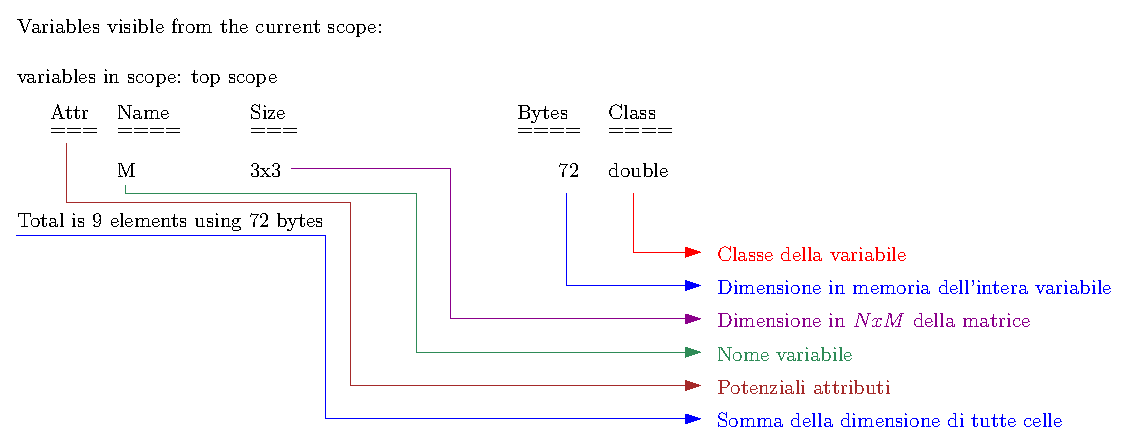
\includegraphics[width=15cm]{img/finiti/whos.eps}
  \caption{descrizione dell'interfaccia di funzione}
  \label{fig:interffun}
\end{figure}
\begin{notab}
  Anche la variabile singola viene vista come una matrice 1x1, da questo si
  denota che come il suo cugino Matlab è un software pensato per elaborare
  prodotti matriciali, infatti, il nome Matlab non sta per \texttt{Mathematic
    lab} ma per \texttt{Matrix Lab}. 
\end{notab}
\subsection{Tipi variabile}
\label{sec:tipivariabile}

\begin{table}[ht]
  \centering
  \begin{tabular}{llll}
    {\bf Nome} & {\bf Descrizione} & {\bf Dimensione} & {\bf Cifre rappresentabili}\\\hline
    \lstinline|double| ({\bf default}) & double-precision array & 8byte & $\pm1.79769x10^{308}$ a $\pm2.22507x10^{-308}$\\\hline
    \lstinline|single| & single-precision array & 4byte & $-2.1475x10^9$ a $2.1475x10^9$\\\hline 
    \lstinline|int8| & Array di interi con segno & 8bit & $-128$ a $127$\\\hline
    \lstinline|int16| & Array di interi con segno & 16bit & $-32768$ a $32767$ \\\hline
    \lstinline|int32| & Array di interi con segno & 32bit & $-2.1475x10^9$ a $2.1475x10^9$\\\hline 
    \lstinline|int64| & Array di interi con segno & 64bit & $-9.2234x10^{18}$ a $9.2234x10^{18}$\\\hline
    \lstinline|uint8| & Array di interi senza segno & 8bit & $255$\\\hline
    \lstinline|uint16| & Array di interi senza segno & 16bit & $65535$ \\\hline
    \lstinline|uint32| & Array di interi senza segno & 32bit & $4.2950x10^9$\\\hline 
    \lstinline|uint64| & Array di interi senza segno & 64bit & $1.8447x10^{19}$\\\hline
  \end{tabular}
  \caption{Tipi variabile}
  \label{tab:tipivariabile}
\end{table}
\begin{oss}
  Questa rapresentazione in memoria vale per la singola cella, quindi bisogna
  moltiplicare il paso per il numero di celle dello stesso tipo. Il programma
  peserà quanto il numero complessivo delle variabili presenti.
\end{oss}

\paragraph{Le stringhe --}
Un altro tipo di variabile però implicita sono le stringhe che il programma può
gestire, nel sequente modo \lstinline|str = "string x"| e la stampa di stringa
viene fatta con un semplice \lstinline|printf(str)|.
\clearpage
\subsubsection{Cosa stampa e cosa no}
Nel linguaggio di Matlab e Octave vengono stampate tutte le associazioni,
funzioni e inizializzazioni che non terminano con il ``{\color{red};}''.

\subsection{Impostazioni e formati}
\label{sec:formImp}
\begin{table}[ht]
  \centering
  \begin{tabular}{lll}
    {\bf Nome} & {\bf Descrizione} & {\bf Visuale}\\\hline
    \lstinline|rat| & Aspetto rateo (invece dei numeri reali rende numeri frazionari) & 1/2\\\hline
    \lstinline|short| & Formato breve a decimale fisso con 4 cifre dopo la virgola. (\textit{default}) & 0.5000\\\hline
    \lstinline|long| & Formato lungo a decimale fisso con 15 cifre dopo la virgola per & 0.500000000000000\\
                     &  i valori doppi e 7 cifre dopo la virgola per i valori singoli. \\\hline
    \lstinline|shortE| & Formato breve in annotazione scientiica con 4 cifre dopo la virgola & 5.0000e-01\\\hline
    \lstinline|longE| & Formato lungo a decimale fisso con 15 cifre dopo la virgola per & 5.000000000000000e-01\\
               & i valori doppi e 7 cifre dopo la virgola per i valori singoli.\\\hline
    \lstinline|shortG| & Formato breve, decimale fisso o notazione scientifica, a seconda & 0.5000\\
               & di quale sia più compatto, con un totale di 5 cifre.\\\hline
    \lstinline|longG| & Formato lungo a decimali fissi o notazione scientifica, qualunque & 0.500000000000000\\
               & sia il più compatto, con un totale di 15 cifre per i valori doppi e\\ & 7 cifre per i valori singoli.\\\hline
    \lstinline|shortEng| & Breve notazione ingegneristica (l'esponente è un
                           multiplo & 500.0000e-003\\
    
               &di 3) con 4 cifre dopo la virgola.\\\hline
    \lstinline|longEng| & Notazione ingegneristica lunga (l'esponente è un multiplo di 3) & 500.000000000000000e-003\\ & con 15 cifre significative.\\\hline
    \lstinline|+|&Formato positivo/negativo con caratteri +, - e vuoti visualizzati & +\\
               & per elementi positivi, negativi e zero.\\\hline
    bank & Formato valuta con 2 cifre dopo la virgola. & 0.50 \\\hline
    hex & Rappresentazione esadecimale di un numero binario & 3fe0000000000000 \\
               & a doppia precisione.\\\hline 
  \end{tabular}
  \caption{Impostazioni e formati}
  \label{tab:form}
\end{table}
\begin{notab}
  È possibile salvare il formato in una variabile con il comando \lstinline|fmt = format("nomeFormato")|
  per poi riutilizzarlo in seguito richiamando \lstinline|format(fmt)|. Altro aspetto esso può cambiare durante lo script quindi è possibile ripotare un dato
  in un formato di stampa e uno in un altro.
\end{notab}

\chapter{Derivate Parziali}
\section{Derivate parziali di primo grado}
\begin{defi}
  Sia $f(x,y)$ una funzione di due variabili definita in un punto interno ad $A$\\
  Consideriamo un interno circolare di $P(x_0,y_0),I(x_0,y_0), \delta$, in netto sulla retta $y=y_0$ e
  incrementa la $x_0$ passante da $x_0$ a $x_0+h$. Ho così un punto $P(x_0+h,y_0)\in A$.\\
  Definisco il rapporto di $f(x,y)$ nella sola $x$
  \begin{equation}
    \frac{f(x_0+h,y_0)-f(x_0,y_0)}{h}
  \end{equation}
  $f(x,y)$ si definisce {\color{red} derivabile parzialmente} se $\exists \lim\limits_{h\to 0}\frac{f(x_0+h,y_0)-f(x_0,y_0)}{h} = l\in R$ reale e finito.
  \begin{equation}
    \frac{\partial f}{\partial x} =fx=\lim\limits_{h\to 0}\frac{f(x_0+h,y_0)-f(x_0,y_0)}{h}
  \end{equation}
  Analogamente, considero un interno di $P(x_0,y_0), I(x_0,y_0),\delta$. Mi ruoto sulla retta $x=x_0$ e
  incremento la $y_0$ passando da $y_0$ a $y_0+k$. Ho così un punto $P(x_0,y_0+h)\in A$.\\
  Definisco il rapporto ingrementale di $f(x,y)$ nella sola $y$
  \begin{equation*}
    \frac{f(x_0+k,y_0)-f(x_0,y_0)}{k}
  \end{equation*}
  {\color{red} derivabile parzialmente} se $\exists \lim\limits_{h\to 0}\frac{f(x_0+h,y_0)-f(x_0,y_0)}{h} =
  l\in R$ reale e finito.\\
  Se in un punto ($x,y$) esistono entrambi le derivate parziale si dice che la funzione è {\color{red} derivabile}
  in (x,y) inoltre se $f$ è derivabile in ogni punto $(x,y)\in A$, si dice che f è derivabile in $A$.
\end{defi}
\subsection{Significato geometrico}
\begin{itemize}
\item Lo derivata prima par parziale in $P$ è $fx(x_0,y_0)$, è la tangente alla curva che si crea intersecando
  $f(x,y)$ con il piano $y=y_0$
\item La derivata prima parziale in $P$, $fy(x_0,y_0)$ è la tangente alla curva che si
  crea intersecando $f(x,y)$ con il piano $x=x_0$
\end{itemize}
Se esistono entrambe allora le due rette tangenti alle sezioni della funzione individuano il piano tangente al
solido nel punto $P(x_0,y_0,z)$
\section{Derivata parziale seconde}
\begin{defi}
  Sia $f(x,y)$ una derivabile e siano definite in un deminio le due derivate parziali
  \begin{equation*}
    \begin{matrix}
      f_x(x,y) & f_y(x,y)
    \end{matrix}
  \end{equation*}
  Tali funzioni passano a loro volta essere derivabili e si ottengono così le derivate seconde parziali di
  $f(x,y)$
  \begin{center}
    \Tree[.$f(x,y)$ [.$f_x(x,y)$ $f_{xx}(x,y)$ $f_{xy}(x,y)$ ] [.$f_y(x,y)$ $f_{yx}(x,y)$ $f_{yy}(x,y)$ ] ]
  \end{center} 
\end{defi}
\begin{multicols}{3}
  \begin{equation*}
    \begin{matrix}
      f_{yx}(x,y)\\
      \text{ derivata prima rispetto a}\\
      \text{ y poi rispetto a rispetto a x}
    \end{matrix}
  \end{equation*}
  \begin{equation*}
    \begin{matrix}
      f_{yx}(x,y)\\
      f_{yx}(x,y)
    \end{matrix}
    \text{ derivata seconde pure}
  \end{equation*}
  \begin{equation*}
    \begin{matrix}
      f_{yx}\\
      f_{yx}
    \end{matrix}
    \text{ derivata seconde resto}
  \end{equation*}
\end{multicols}
con $n$ variabili si hanno $n^2$ derivate seconde parziali -- Spesso le derivate seconde sono disposte in
una matrice quadrata, detta {\tt hessiana}, con il sinbolo $D^2$
\begin{equation}
  D^2f=\begin{bmatrix}
         f_{xx} & f_{xy}\\
         f_{yx} & f_{yy}
       \end{bmatrix}
       \text{n variabili} \to n*n
\end{equation}
Se esistono le quanto derivate di f, nel punto (x,y), si dice che $f$ è dirivabile due volte in $(x,y)$. Se
ciò accade $\forall (x,y)\in A$, $f$ è derivabile due volte nell'insieme A.
\subsection{Teorema di Schwarz (Dell'invertibilità dell'ordine di derivazione)\label{Schwarz}}
\begin{teorema}
  Sia $f(x,y)$ definita in $D$ e derivabile due volte $\forall (x,y) \in D$.\\
  Se le derivate seconde in $(x_0,y_0)$ $f_{xy}(x_0,y_0)$ e $f_{yx}(x_0,y_0)$ sono continue in ($x_0,y_0$) allora\\
  risulta $f_{xy}(x_0,y_0)=f_{yx}(x_0,y_0)$.
\end{teorema}
In generale se vale il teorema di Schwarz, la matrice Hessiana può essere scritta come
\begin{equation*}
  H=D^2f=\begin{bmatrix}
           f_{xx} & f_{xy}\\
           f_{xy} & f_{yy}
         \end{bmatrix}
         = \begin{bmatrix}
             f_{xx} & f_{yx}\\
             f_{yx} & f_{yy}
           \end{bmatrix}
\end{equation*}
$det H= f_{xx}*f_{yy}-(f_{xy})^2=f_{xx}*f_{yy}-(f_{yx})^2$
\section{Massimi e minimi relativi \label{minmaxrel}}
\begin{defi}
  Sia $f(x,y)$ una funzione definita in un insieme D, un punto $p_0(x_0,y_0)\in D$, si dice di {\color{red}
    massimo relativo} per la funzione se esiste intorno circolare di $P_0$ per cui il valore assunto della
  funzione nei punti dell'interno è minore o uguale a quello assunto in $P_0$.\\
  Analogamente un punto $P_0(x_0,y_0)$ si dice di {\color{red} minimo relativo} per la funzione se esiste un
  interno circolare di $P_0$ per cui il valore assunto dalla funzione nei punti dell'intorno è maggiore o uguale.
  \begin{equation*}
    \begin{matrix}
      \exists I_{(x,y),\delta}:\forall (x,y)\in I_{(x,y),\delta} & f(x_0,y_0)\geq f(x,y) & \text{Massimo relativo}\\
      \exists I_{(x,y),\delta}:\forall (x,y)\in I_{(x,y),\delta} & f(x_0,y_0)\leq f(x,y) & \text{Minimo relativo}
    \end{matrix}
  \end{equation*} 
\end{defi}
\subsection{Teorema di Fermat}
\begin{teorema}
  Sia $f(x,y)$ derinita in D e derivabile in un punto $P_0 (x_0,y_0)$\\
  Se in $P_0(x_0,y_0)$ $f(x,y)$ ha un massimo o un minimo relativo, allora le derivate prime
  parziali si annullano ($\nabla f=0$ gradiente nullo). La pendenza della tangente è zaro un
  massimo o minimo.
\end{teorema}
\subsubsection{Gradiente}
Sia $f(x,y)$ una funzione derivabile in un punto (x,y), cioè esistano in (x,y) le due derivate
parziali $f_x$ e $f_y$.\\
Si definisce {\color{red} gradiente} di f(x,y) nel punto (x,y): i vettore $\nabla f$ le cui componenti sono le derivate parziali di f(x,y).
\begin{equation}
  \nabla f(x,y) \equiv (f_x(x,y); f_y(x,y))
\end{equation}
\subsubsection{Massimi e minimi -- condizione necessaria}
\begin{defi}
  Se $P_0(x_0,y_0)$ è un punto di massimo/minimo relativo il gradiente è nullo. Così di massimo
  o minimo relativo interni al dominio della funzione f vanno ricercati tra i punti che annullano
  la funzione f. Pertanto un punto critico per una funzione derivabile e un punto in cui si
  annulla il gradiente della funzione.
\end{defi}

\chapter{Differenziabilità}
\begin{defi}
  Sia $f(x,y)$ definita in D e $P_0(x_0,y_0)\in D$. In $P_0, z=f(x_0,y_0)$, incremento la $x_0$
  di un h e la $y_0$ di un k.\\
  Così passo da $P_0(x_0,y_0)$ a $P(x_0+h,y_0+k)$. La funzione avrà avuto un certo incremento
  \begin{equation*}
    f(x+h,y_0,y_0+k)-f(x_0,y_0)
  \end{equation*}
  Si definisce {\color{red}differenziale} in $P_0(x_0,y_0)$ se
  $\exists A,B \in R: f(x_0+h,y_0+k)-f(x_o,y_0)=Ah+Bk+o(\sqrt{h^2+k^2})$, cioè se esistono
  due costanti reali A e B per cui l'increm,ento di $f(x,y)$ che si ha passando da $P_0$ a $P$
  si può riscrivere come somma di una parte lineare $Ah+Bk$ e di un infinitesimo di ordine
  superiore a $\sqrt{h^2+k^2}$ (\underline{distanza di $P_0$ da $P$}).\\
  Se $f(x,y)$ ammette derivate prime parziali le due costanti A e B sono:
  \begin{equation*}
    \begin{cases}
      A=fx(x_0,y_0)\\
      B=fy(x_0,y_0)
    \end{cases}
  \end{equation*}
  e il differenziale diventa
  \begin{equation}
    f(x_0+h,y_0+k) - f(x_0,y_0)=fx(x_0,y_0)h+fy(x_0,y_0)k+o(\sqrt{h^2+k^2})
  \end{equation}
\end{defi}
\begin{esempio}
  verificare che $z=xy$ è differenziale $\forall (x_0;y_0)\in R^2$, se z è differenziale\\
  $\to f(x_0+h,y_0+k) - f(x_0,y_0)=fx(x_0,y_0)h+fy(x_0,y_0)k+o(\sqrt{h^2+k^2})$ dove
  \begin{equation*}
    \begin{cases}
      A=fx(x_0,y_0)\\
      B=fy(x_0,y_0)
    \end{cases}
  \end{equation*}
  se z è derivabile in ($x_0,y_0$).
  \begin{equation*}
    f(x_0+h,y_0+k) =\underbrace{(x_0+h)(y_0+k)}_{\text{\shortstack{Sostituisco}}}=x_0y_0+x_0k+y_0h+hk
  \end{equation*}
  \begin{multicols}{3}
    $f_x=y\text{ }fx(x_0,y_0)=y_0$\\
    $f$ è derivabile in $(x_0,y_0)$\\
    $f_y=x$\\
    $A=y_0$\\
    $f_y(x_0,y_0)=x_0$\\
    $D=x_0$
  \end{multicols}
  \begin{equation*}
    \begin{matrix}
      f(x_0+h,y_0+k) - f(x_0,y_0)=Ah+Bk+o(\sqrt{h^2+k^2})\\
      \not{x_0y_0}+\not{x_0k}+hk-\not{x_0y_0}=\not{y_0h}+\not{x_0k}+o(\sqrt{h^2+k^2})\\
      hk=o(\sqrt{h^2+k^2})
    \end{matrix}
  \end{equation*}
  detto quindi dimostrare che $\lim\limits_{h\to 0 k\to 0}\frac{hk}{\sqrt{h^2+k^2}}=0$
  e poi passo alle coordinate polari:
  \begin{equation*}
    \begin{matrix}
      h=\rho \cos \theta\\
      k=\rho \sin \theta & \lim\limits_{\rho\to 0} \frac{\not{e} \cos\theta* \not{e} sin\theta}{\not{e}^2}& z=xy \text{ defferenziale } \forall (x_0,y_0)\in R^2\\
      e^2=h^2+k^2\\
      h\to0,k\to 0,\rho \to 0\\
    \end{matrix}
  \end{equation*}  
\end{esempio}
\subsection{Tutte le funzioni differenziali sono continue}
Sia $f(x,y)$ differenziabile $(x_0,y_0)$, allora $f(x,y)$ è continua in $(x_0,y_0)$
\begin{multicols}{2}
  \paragraph{Ip:}
  \begin{equation*}
    f(x,y) \text{ differenziabile in } (x_0,y_0)
  \end{equation*}
  \paragraph{Th:}
  \begin{equation*}
    f(x,y) \text{ è continua in } (x_0,y_0)
  \end{equation*}
\end{multicols}
\begin{proof}
  Poiché $f(x,y)$ è differenziabile in ($x_0,y_0$) vale la relazione
  \begin{equation*}
    f(x_0+h,y_0+k) - f(x_0,y_0)=Ah+Bk+o(\sqrt{h^2+k^2})
  \end{equation*}
  Se $f(x_0,y_0)$ è continua in $(x_0,y_0)$
  \begin{equation*}
    \lim_{h\to 0\text{ } k\to 0}f(x_0+h,y_0+k) - f(x_0,y_0)=0
  \end{equation*}
  Calcolo il limite a destra per $h\to 0$ $k\to 0$
  \begin{equation*}
    \lim_{h\to 0\text{ } k\to 0}\underbrace{Ah}_0+\underbrace{Bk}_0+o\underbrace{(\sqrt{h^2+k^2})}_0=0 \text{ per cui $f(x,y)$ è continua in ($x_o,y_0$)}
  \end{equation*} 
\end{proof}
\subsection{Tutte le funzioni differenziali sono derivabili}
Sia $f(x,y)$ differenziabile in un punto ($x_0,y_0$). Allora $f(x,y)$ è derivabile in
$(x_0,y_0)$
\begin{multicols}{2}
  \paragraph{Ip:}
  \begin{equation*}
    f(x,y) \text{ differenziabile in } (x_0,y_0)
  \end{equation*}
  \paragraph{Th:}
  \begin{equation*}
    f(x,y) \text{ è derivabile in } (x_0,y_0)
  \end{equation*}
\end{multicols}
\begin{proof}
  Poiché $f(x,y)$ è differenziabile in ($x_0,y_0$) vale la relazione
  \begin{equation*}
    f(x_0+h,y_0+k) - f(x_0,y_0)=Ah+Bk+o(\sqrt{h^2+k^2})
  \end{equation*}
  divido entrambi per h e calcolo il limite per $h\to 0$
  \begin{equation*}
    \lim\limits_{h \to 0}\underbrace{\frac{f(x_0+h,y_0) - f(x_0,y_0)}{h}}_{\frac{\partial f}{\partial x}(x_0,y_0)=fx}=\underbrace{\frac{Ah+o(\sqrt{h^2})}{h}}_A
  \end{equation*}
  $fx(x_0,y_0)=A$\\
  Analogamente si demostra che $f_y(x_0,y_0)=B$. Qundi dato che esistono $f_x$ e $f_y$ in ($x_0,y_0$), $f(x,y)$ è derivabile in $(x_0,y_0)$ e in oltre $A=fx(x_0,y_0)$, $B=fy(x_0,y_0)$
\end{proof}
\begin{esercizio}
  Dimostrare che $z=x^2=y^2$ è differenziabile in (1;1) -- Per definire
  \begin{equation*}
    f(x_0+h,y_0+k)-f(x_0,y_0)=Ah=Bk+o(\sqrt{h^2+k^2})
  \end{equation*}
  \begin{multicols}{2}
    $f(x_0+h,y_0+k)=(1+h)^2=(1+k)^2$\\
    $A=f(1,1)=\abs{2x}_{x=1}=2$\\
    $f(x_0,y_0)=1+1=2$\\
    $B=f_y(1,1)=\abs{2y}_{y=1}=2$
  \end{multicols}
  Così ho $(1+h)^2+(1+k)^2-2=2h+2k+o(\sqrt{h^2+k^2})$
  \begin{equation*}
    h^2+k^2=o(\sqrt{h^2+k^2})
  \end{equation*}
  devo dimostrare che $\lim\limits_{h\to 0\text{ } k\to0}\frac{h^2+k^2}{\sqrt{h^2+k^2}}=0$ pasando
  a coordinate polari $\begin{matrix} h=e\cos \theta\\ k=e\sin \theta\\ e^2=h^2+k^2\\ k\to 0,h\to 0,
                         p\to 0\end{matrix}$\\ 
                       $\lim\limits_{e\to 0}\frac{e^2}{\abs e}=0 \to z=x^2+z^2$ è differeziabile in (1,1)
\end{esercizio}
\subsection{Le funzioni con derivate parziali continue sono diferenziabili}
\begin{defi}
  Sia $f(x,y)$ definita in $D_1$ e sia derivabile in $D$. Sono $f_x$ e $f_y$ continue in $D$, allora
  $f(x,y)$ è differenziale in $D$.
\end{defi}
\subsubsection{Condizione sufficiente per la differenzialità}
\begin{defi}
  Affinché una funzione sia differenziabile in $(x_0,y_0)$ basta che in $(x_0,y_0)$ abbia derivate.
  In questo modo per determinare se una funzione è differenziabile in un punto si calcola le
  derivate parziali in quel punto, se esistono la funzione è differenziabile, in caso contrario
  non è derivabile.
\end{defi}
\begin{esempio}
  Dimostrare che $z=\sqrt{x^2+y^2}$ non è differenziabile in (0;0)
  \begin{equation*}
    \begin{matrix}
      z_x=\frac{2x}{2\sqrt{x^2+y^2}} = \frac{x}{\sqrt{x^2+y^2}} & D: x^2+y^2>0 \\
      z_y=\frac{2y}{2\sqrt{x^2+y^2}} = \frac{y}{\sqrt{x^2+y^2}} & D: x^2+y^2>0
    \end{matrix}
  \end{equation*}
  Sia $z_x$ sia $z_y$ sono definite per $x^2+y^2>0$ cioè nei punti esterni al cerchio di centro (0,0)
  e 1, frontiera eclusa. Il punto (0,0) è interno al cerchio, quindi in esso $f(x,y)$ non è derivabile. Per cui in punto (0,0) f(x,y) non è neanche differenziabile.
\end{esempio}
\section{Significato geometrico del differenziale e piano tengente}
\subsection{Differenziale primo}
È la parte lineare nella definizione di differenziale
\begin{equation*}
  \begin{matrix}
    f(x,y) \text{ definita in } D & (x_0,y_0)\in D
  \end{matrix}
\end{equation*}
$f(x,y)$ differenziale in $(x_0,y_0)$ se
\begin{equation*}
  f(x_0+h,y_0+_k)-f(x_0,y_0)=\underbrace{f_x(x_0,y_0)h+f_y(x_0,y_0)k}_{\text{parte lineare}}
  +o(\sqrt{h^2+k^2})
\end{equation*}
\begin{equation*}
  df(x_0,y_0)=f_x(x_0,y_0)h+f_y(x_0,y_0)k
\end{equation*}
\subsection{Piano Tangente}
La $f(x,y)$ una funzione derivabile in $(x_0,y_0)$, il piano tangente alla funzione $(x_0,y_0,z_0)$
ha equazione:
\begin{equation*}
  z-z_0=f_x(x_0,y_0)(x-x_0)+f_y(x_0,y_0)(y-y_0)
\end{equation*}
$\vec{n}$ direzione ortogonale al piano tangente, è unitario
\begin{equation*}
  \vec{n}=\frac{(-f_{x_i}-f_{y_i}1)}{\sqrt{1+f_x^2+f_y^2}}
\end{equation*}
poiché $\nabla f(f_x,f_y)$ $\abs{\nabla f}^2=f_x^2+f_y^2\to \vec{n}=\frac{(-f_{x_i}-f_{y_i}1)}{\sqrt{1+\abs{\nabla f}}}$
\begin{esempio}
  $z=x^2+y^2$ (1,1)
  \begin{equation*}
    z-z_0=f_x(x_0,y_0)(x-x_0)+f_y(x_0,y_0)(y-y_0)
  \end{equation*}
  \begin{equation*}
    \begin{matrix}
      z_0=f(1,1)=1+1=2 & z-2=2(x-1)+2(y-1) & f_x=2x|_{1_{ii}}=2\\
                       & & f_y=2y|_{1_{ii}}=2
    \end{matrix}
  \end{equation*}
\end{esempio}
\subsection{Significato geometrico del differenziale primo}
Passando da $P_0$ a $P$ $f(x)$ si incrementa da $f(x_0)$ a $f(x_0+h)$ -- Il differenziale primo $dy$
indica la variazione che subisce la retta tangente passando da $P_0$ a $P$.\\
L'incremento $f(x_0+h)-f(x_0)$ si approssima sempre più con $dy$ per incrementi $h\to 0$
\begin{equation*}
  f(x_0+h)-f(x_0)=f^\prime (x)(x-x_0)-f(x_0)+o\abs{x}
\end{equation*}
L'incremento $f(x_0+h)-f(x_0)$ differisce dal valore $f^\prime (x)(x-x_0)$ [retta tangente] per un
$o\abs{x}$, $o\abs{x}$ ci da l'errore.
\subsection{Funzioni composite}
\begin{defi}
  Sia $x(t)$ E $y(t)$ due funzioni reali definite al variare in un intervallo $I$ di $R$.
  $t\in T \leq R$ corrisponde il punto $(x(t),y(t))$
  \begin{equation*}
    \begin{cases}
      x=x(t) & \text{Rappresenta nel piano una currva in frontiera}\\
      y=y(t) & \text{Parametrica}
    \end{cases}
  \end{equation*}
  Al variare di $t\in I\leq R$\\
  $x=x(t),y=y(t)$ descrive una curva $\gamma$ nel piano 
\end{defi}
\clearpage
\begin{esempio}
  \begin{equation*}
    \begin{matrix}
    \begin{cases}
        x=t-1\\
        y=t+1
    \end{cases}& t\in [0,1] &
    \begin{cases}
        x=\Gamma \cos t\\
        y=\Gamma \sin t
    \end{cases}& t\in [0,2\pi]\\
      y=(t-1)+2=x+2 && r^2\cos t+ r^2\sin^2t=r^2
    \end{matrix}
  \end{equation*}
  \begin{multicols}{2}
    \begin{tikzpicture}[scale=2]
        \draw[step=.5cm, gray, very thin] (-1.2,-1.2) grid (1.2,1.2); 
        \draw[->] (-1.25,0) -- (1.25,0) coordinate (x axis);
        \draw[->] (0,-1.25) -- (0,1.25) coordinate (y axis);
        \draw (0,0) circle (1cm);
        \foreach \x/\xtext in {-1, -0.5/-\frac{1}{2}, 1} 
        \draw (\x cm,1pt) -- (\x cm,-1pt) node[anchor=north,fill=white] {$\xtext$};
        \foreach \y/\ytext in {-1, -0.5/-\frac{1}{2}, 0.5/\frac{1}{2}, 1} 
        \draw (1pt,\y cm) -- (-1pt,\y cm) node[anchor=east,fill=white] {$\ytext$};
      \end{tikzpicture}
      \begin{equation*}
      	[x(t)]^2+[y(t)]^2=r^2
      \end{equation*}
      circonferenza con certro nel origine e raggio r
    \end{multicols}
    Se si ha $\begin{cases} x=x(t) \\ y=y(t) \\ z=z(t)\end{cases}$ al variare di $t\in T \leq R$ si
    ha una curva nello spazio.
\end{esempio}
\begin{esempio}
  $\begin{cases} x = \Gamma \cos t \\ y = \Gamma \sin t \\ z=Kt \end{cases}$ elica circolare 
\end{esempio}
\subsection{Funzione composta}
\begin{defi}
  Sia $\gamma$ la curva $\begin{cases} x=x(t) \\ y=y(t)\end{cases}$ $t\in I < R$
	di codominio B\\
  $I\to B$\\
  Sia f(x,y) definita in A \\
  $t\in f(x(t),y(t))$ se il codominio di $\gamma$ coincide con il codomio di
	$f(x,y)$, cioè
  $B \leq A$
\end{defi}
\subsection{Teorema della derivata della funzione composta}
\begin{defi}
	Sia $\gamma$ la curva di punti $(x(t),y(t))$ e sia derivabile in un
	intervallo $I$ (\underline{cioè esistono })\\
	Sia f(x,y) differenziabile in x(t)\\
	Allora la funzione conposta da $F(t)=f(x(t),y(t))$ è derivabile in I e la
	sua derivata prima vale:
	\begin{equation}
		F^\prime (t)=f_x(x(t),y(t))x^\prime(t)+f_y(x(t),y(t))y^\prime(t)
	\end{equation}
	\begin{equation*}
		\begin{matrix}
			(\nabla f *\Gamma^\prime (t)) & \nabla f \equiv (f_x;f_y) &
			\Gamma^\prime \equiv(x^\prime (t); y^\prime (t))
		\end{matrix}
	\end{equation*}
	\begin{multicols}{2}
		\paragraph{Ipotesi}
			$\gamma \equiv (x(t),y(t))$ derivabile in I\\
			$f(x,y)$ differenziale in x(t)
		\paragraph{Tesi}
		$F(t)=f(x(t),y(t))$ derivabile in I\\
		$F^\prime(t)=f_x(x(t),y(t))x^\prime(t)+f_y(x(t),y(t))y^\prime (t)$
	\end{multicols}
\end{defi}
\begin{proof}
	Devo dimostrare che $\lim\limits_{h\to 0} \frac{F(t+h)-F(t)}{h}=F^\prime
	(t)=F_x(x(t),y(t))x^\prime (t)+f_y(x(t),y(t))y^\prime(t)$\\
	Scrivo l'incremento di F(t) per un h
	\begin{equation*}
		F(t+h)-F(t)=f[x(t+h),y(t+h)]- f[x(t), y(t)] \text{ Per definizione di funzione composta F(t)}
	\end{equation*}
	Poiché f(x,y) è differenziabile si ha 
	\begin{equation*}
		\begin{matrix}
			f[x(t+h),y(t+h)]-f[x(t),y(t)]=f_x\underbrace{[x(t),y(t)]}_{fx}
			\underbrace{[x(t+h)-x(t)]}_h+
			f_y\underbrace{[x(t+h)-y(t+h)]}_{fy}\underbrace{[y(t+h)-y(t)]}_k\\+o
			\left(\sqrt{\underbrace{[x(t+h)-x(t)]^2}_{h^2}
			+  \underbrace{[y(t+h)-y(t)]^2}_{k^2}}\right)
		\end{matrix}
	\end{equation*}
	Divido entrambi i membri per h e calcolo il $\lim_{h\to 0}$
	\paragraph{I membro}
	\begin{equation*}
		\lim_{h\to 0} \frac{f[x(t+h),y(t+h)]-f[x(t),y(t)]}{h}=F^\prime(t)
	\end{equation*}
	\paragraph{II membro}
	\begin{equation*}
		\begin{matrix}
			\lim\limits_{h\to
		0}fx[x(t),y(t)]\underbrace{\left[\frac{x(t+h)-x(t)}{h}\right]}_{x^\prime
		(t)} + \lim\limits_{h\to 0} f_y
		[x(t+h)-y(t+h)]\underbrace{\left[\frac{y(t+h)-y(t)}{h}\right]}_{y^\prime
		(t)}\\ +\lim\limits_{h\to 0}o
			\underbrace{\left(\sqrt{[x(t+h)-x(t)]^2 +
			[y(t+h)-y(t)]^2}\right)}_0
		\end{matrix}
	\end{equation*}
	\begin{equation*}
		F^\prime =f_x[x(t),y(t)]x^\prime(t)+f_y[x(t),y(t)]y^\prime (t)
	\end{equation*}
\end{proof}
\begin{esempio}
	\begin{equation*}
		\begin{matrix}
			z=x^2y & \begin{cases}
				x(t)=-t & F(t)=z(x(t),y(t))=-t^2*t=-t^3\\
				y(t)=t & F^\prime(t)=z^\prime=-3t^2
			\end{cases}
		\end{matrix}
	\end{equation*}
	\begin{equation*}
		F^\prime(t)=f_x(x(t), y(t))x^\prime(t)+f_x(x(t), y(t))y^\prime (t)=z_x
		x^\prime(t)+z_y y^\prime(t) = -3t^2
	\end{equation*}
\end{esempio}
\section{Teorema differenziabilità delle funzioni composite}
\begin{teorema}
	Siano $x=(x_1,x_2,\dots,x_n)$ n funzioni in k variabili
	$t=(t_1,t_2,\dots,t_k)$
	\begin{equation}
		\begin{cases}
			x_1=x_1(t_1,t_2,\dots,t_k)\\
			x_2=x_2(t_1,t_2,\dots,t_k)\\
			\dots\\
			x_n=x_n(t_1,t_2,\dots,t_k)
		\end{cases}
	\end{equation}
	Componiamo le funzioni ottenendo la funzione composita
	\begin{equation*}
		f[x_1(t_1,t_2,\dots,t_k), x_2(t_1,t_2,\dots,t_k), \dots,
		x_n(t_1,t_2,\dots,t_k)]
	\end{equation*}
	Siano ($x_1(t_1,t_2,\dots,t_k), x_2(t_1,t_2,\dots,t_k), \dots,
		x_n(t_1,t_2,\dots,t_k)$) n funzioni definite in un insieme aperto
		$D\leq R^n$ e siano derivabili parzialmente rispetto a $t_i$
		($i=1,2,\dots, k$).\\
		Sia $f(x_1,\dots,x_n)$ una funzione definita in A contenente in
		codominio $x(D)$ e sia f differenziabile in A\\
	Allora la funzione composita $F(t)=x_1(t_1,t_2,\dots,t_k), x_2(t_1,t_2, 
		\dots,t_k), \dots, x_n(t_1,t_2,\dots,t_k)$ è derivabile parzialmente
		rispetto a $t_i(i=1,2,\dots,k)$ nel punto t.
		\begin{equation*}
			\frac{\partial F}{\partial t_i} (t)=\frac{\partial f}{\partial
			x_j}(x(t))+\frac{\partial x_i}{\partial t_i}(t) \text{ (si somma
			sugli inasci ripetuti)}
		\end{equation*}
		Inoltre, se f e ($x_1(t_1,t_2,\dots,t_k), x_2(t_1,t_2,\dots,t_k), \dots,
		x_n(t_1,t_2,\dots,t_k)$) sono di classe $C^1$, anche $F=f(x(t))\in c^1$
		ed è quindi differenziabile.
		\begin{equation*}
			\hbar=k=2 \text{ coordinate polari}
		\end{equation*}
		\begin{equation*}
			\begin{matrix}
				\begin{cases}
					x_1=x\\
					x_2=y
				\end{cases}
				\begin{cases}
					t_1=\varphi\\
					t_2=\varphi
				\end{cases} & f(x,y) &
				\begin{cases}
					x=x(\varphi,\varphi)\\
					y=y(\varphi,\varphi)
				\end{cases}\to \begin{cases}
					x=\rho\cos \varphi\\
					y=\rho \sin \varphi
				\end{cases}
			\end{matrix}
		\end{equation*}
		\begin{equation*}
			f(x,y)=f(\rho\cos\varphi,\rho \sin \varphi)
		\end{equation*}
		\begin{equation*}
			\begin{matrix}
				\frac{\partial f}{\partial \rho}=\frac{\partial f}{\partial x}
				x\rho+\frac{\partial f}{\partial y}y\rho=
				\frac{\partial f}{\partial x} \cos \varphi+
				\frac{\partial f}{\partial y} \sin \varphi\\
				\frac{\partial f}{\partial \rho}=\frac{\partial f}{\partial x}
				x\rho+\frac{\partial f}{\partial y}y\varphi=
				\frac{\partial f}{\partial x} (-\rho\sin \varphi)+
				\frac{\partial f}{\partial y} (\rho\sin \varphi)
			\end{matrix}
		\end{equation*}
\end{teorema}
\section{Differenziale secondo}
\begin{defi}
	$d^2f$ è il differenziale del differenziale primo
        \begin{equation*}
                \begin{matrix}
                        d^2f=d(df)= d(f_xh+f_yk)=\frac{\partial}{\partial x} (f_xh+f_yk)h+ 
                        \frac{\partial}{\partial x}(f_xh+f_yk)k=\\
                        =(f_{xx}h+f_{xy}k)h+ (f_{xy}h+f_{yy}k)k=f_{xx}h^2+f_{xy}k hx+ f_{xy}
                        hx+f_{yy} k^2
                \end{matrix}
         \end{equation*}
         Se $f(x,y)\in c^2$ (derivate parziali II continue) vale il teorema di Schwarz
         (\ref{Schwarz}), cioè $fyx=fxy$ -- Il differenziale secondo allora diventa
         \begin{equation*}
           d^2f=fxxh2+3fxy hk + fyy k^2
         \end{equation*}
         Per ipotesi il gradiente è nulla $\Delta f(x_0,y_0)=0$ cioè $\nabla f(x_0,y_0)\equiv (f_x(x_0,y_0),fy(x_0,y_0))\equiv (0,0)$ ovvero le derivate parziali prime sono nulle
         $fx(x_0,y_0)=0$, $fy(x_0,y_0)=0$ -- Ciò comporta l'annullarsi del differenziale primo
         \begin{equation*}
           df(x_0, y_0)=fx(x_0,y_0)h+fy(x_0,y_0)k=0*h+0*k=0
         \end{equation*}
         Per cui nella foruma di Taylor si ha:
         \begin{equation*}
           f(x,y)=f(x_0,y_0)+\frac{1}{2!}d^2f(x_0+\theta h, y_0+\theta k) \text{ Forme quadratiche}
         \end{equation*}
         Il segno di $f(x,y)-f(x_0,y_0)$ è lo stesso di $\frac{1}{2!}d^2f(x_0+\theta h,
         y_0+\theta k)$, cioè è lo stesso differenziale secondo.\\
         Per ipotesi $det Hp(x_0,y_0)>0$, ($f(x,y)\in C_A^2\Rightarrow$ vale il teorema di Schwarz)
         \begin{equation*}
           \begin{vmatrix}
             fxx(x_0,y_0) & fxy(x_0,y_0) \\
             fyx(x_0,y_0) & fyy(x_0,y_0) 
           \end{vmatrix}= fxx*fyy-fxy^2>0
         \end{equation*}
         e $fxx(x_0,y_0)>0$\\
         Ciò implica per definizione che la forma quadratica associata ad $Hp(x_0,y_0)$ è positiva
         tutto ciò implica $d^2f(x_0+\theta h, y_0+\theta k)>0$\\
         Per cui $f(x,y)-f(x_0,y_0)>0$ 
         \begin{equation*}
           \begin{matrix}
              \text{cioè } f(x,y)>f(x_0,y_0) & \text{ difiniziondi di Minimo relativo (\ref{minmaxrel})}
           \end{matrix}
         \end{equation*}
         quindi $(x_0,y_0)$ è un punto di muinimo relativo\\
         Analogamente, se $f(x_0,y_0)<0$ si dimosta che $(x_0,y_0)$ è un punto di massimo
         relatovo (\ref{minmaxrel})
\end{defi}
\clearpage
\subsection{Condizioni sufficiente per l'esistenza di minimo e massimo relativo}
Sia $f(x,y)$ definita in $A,\text{ } f(x,y)\in C^2_A, \text{ } (x_0,y_0)\in A$\\
Se $\nabla f(x_0,y_0)=0$
\begin{equation*}
  det H_F(x_0,y_0)\begin{cases}
                    >0 \begin{cases}
                         fxx(x_0,y_0)>0 \text{ \color{red} Minimo relativo}\\
                         fxx(x_0,y_0)<0 \text{ \color{red} Massimo relativo}
                       \end{cases}\\
                    <0 \text{ Punto di sella (\underline{non sono presenti Max e min})}\\
                    =0 \text{ Non si vsa se sono presenti Max o min}
                  \end{cases}
\end{equation*}
\begin{esempio}
  Massimi e minimi
  \begin{enumerate}
  \item $z=x^2+y^2$
    \begin{equation*}
      \nabla f=0 \begin{cases}
                   zx=0\\
                   zy=0
                 \end{cases}\begin{cases}
                   2x=0\\
                   -2y=0
                 \end{cases}\begin{cases}
                   x=0\\
                   y=0
                 \end{cases} in (0,0)\text{ }\nabla f=0 \text{ può MAX o MIN}
    \end{equation*}
    \begin{equation*}
		det H_f=\begin{vmatrix}
			z_{xx} & z_{zy} \\
			z_{xy} & z_{yy}
		\end{vmatrix}=\begin{vmatrix}
			2 & 0 \\
			0 & -2
		\end{vmatrix} =-4
    \end{equation*}
    \item Semisuperfici sferica $z=\sqrt{c^2-x^2-y^2}$
		\begin{equation*}
			\nabla f=0 \begin{cases}
				z_x=\frac{-x}{\sqrt{\Gamma^2-x^2-y^2}}\\
				z_y=\frac{-y}{\sqrt{\Gamma^2-x^2-y^2}}
			\end{cases} \text{ dominio D } x^2-y^2<\Gamma^2 
		\end{equation*}
		\begin{equation*}
			\begin{cases}
				z_x=0\\
				z_y=0
			\end{cases}\begin{cases}
					x=0\\
					y=0
			\end{cases} (0,0)\leftarrow D \text{ può esserci un Max e un Min}
		\end{equation*}
		  Verifico e trovo che $det H>0$ $f_{xx}<0: in(0,0)$ è presente il Max.
	  \item Cono $z=\sqrt{x^2+y^2}$ 
		\begin{figure}[ht]
			\centering
			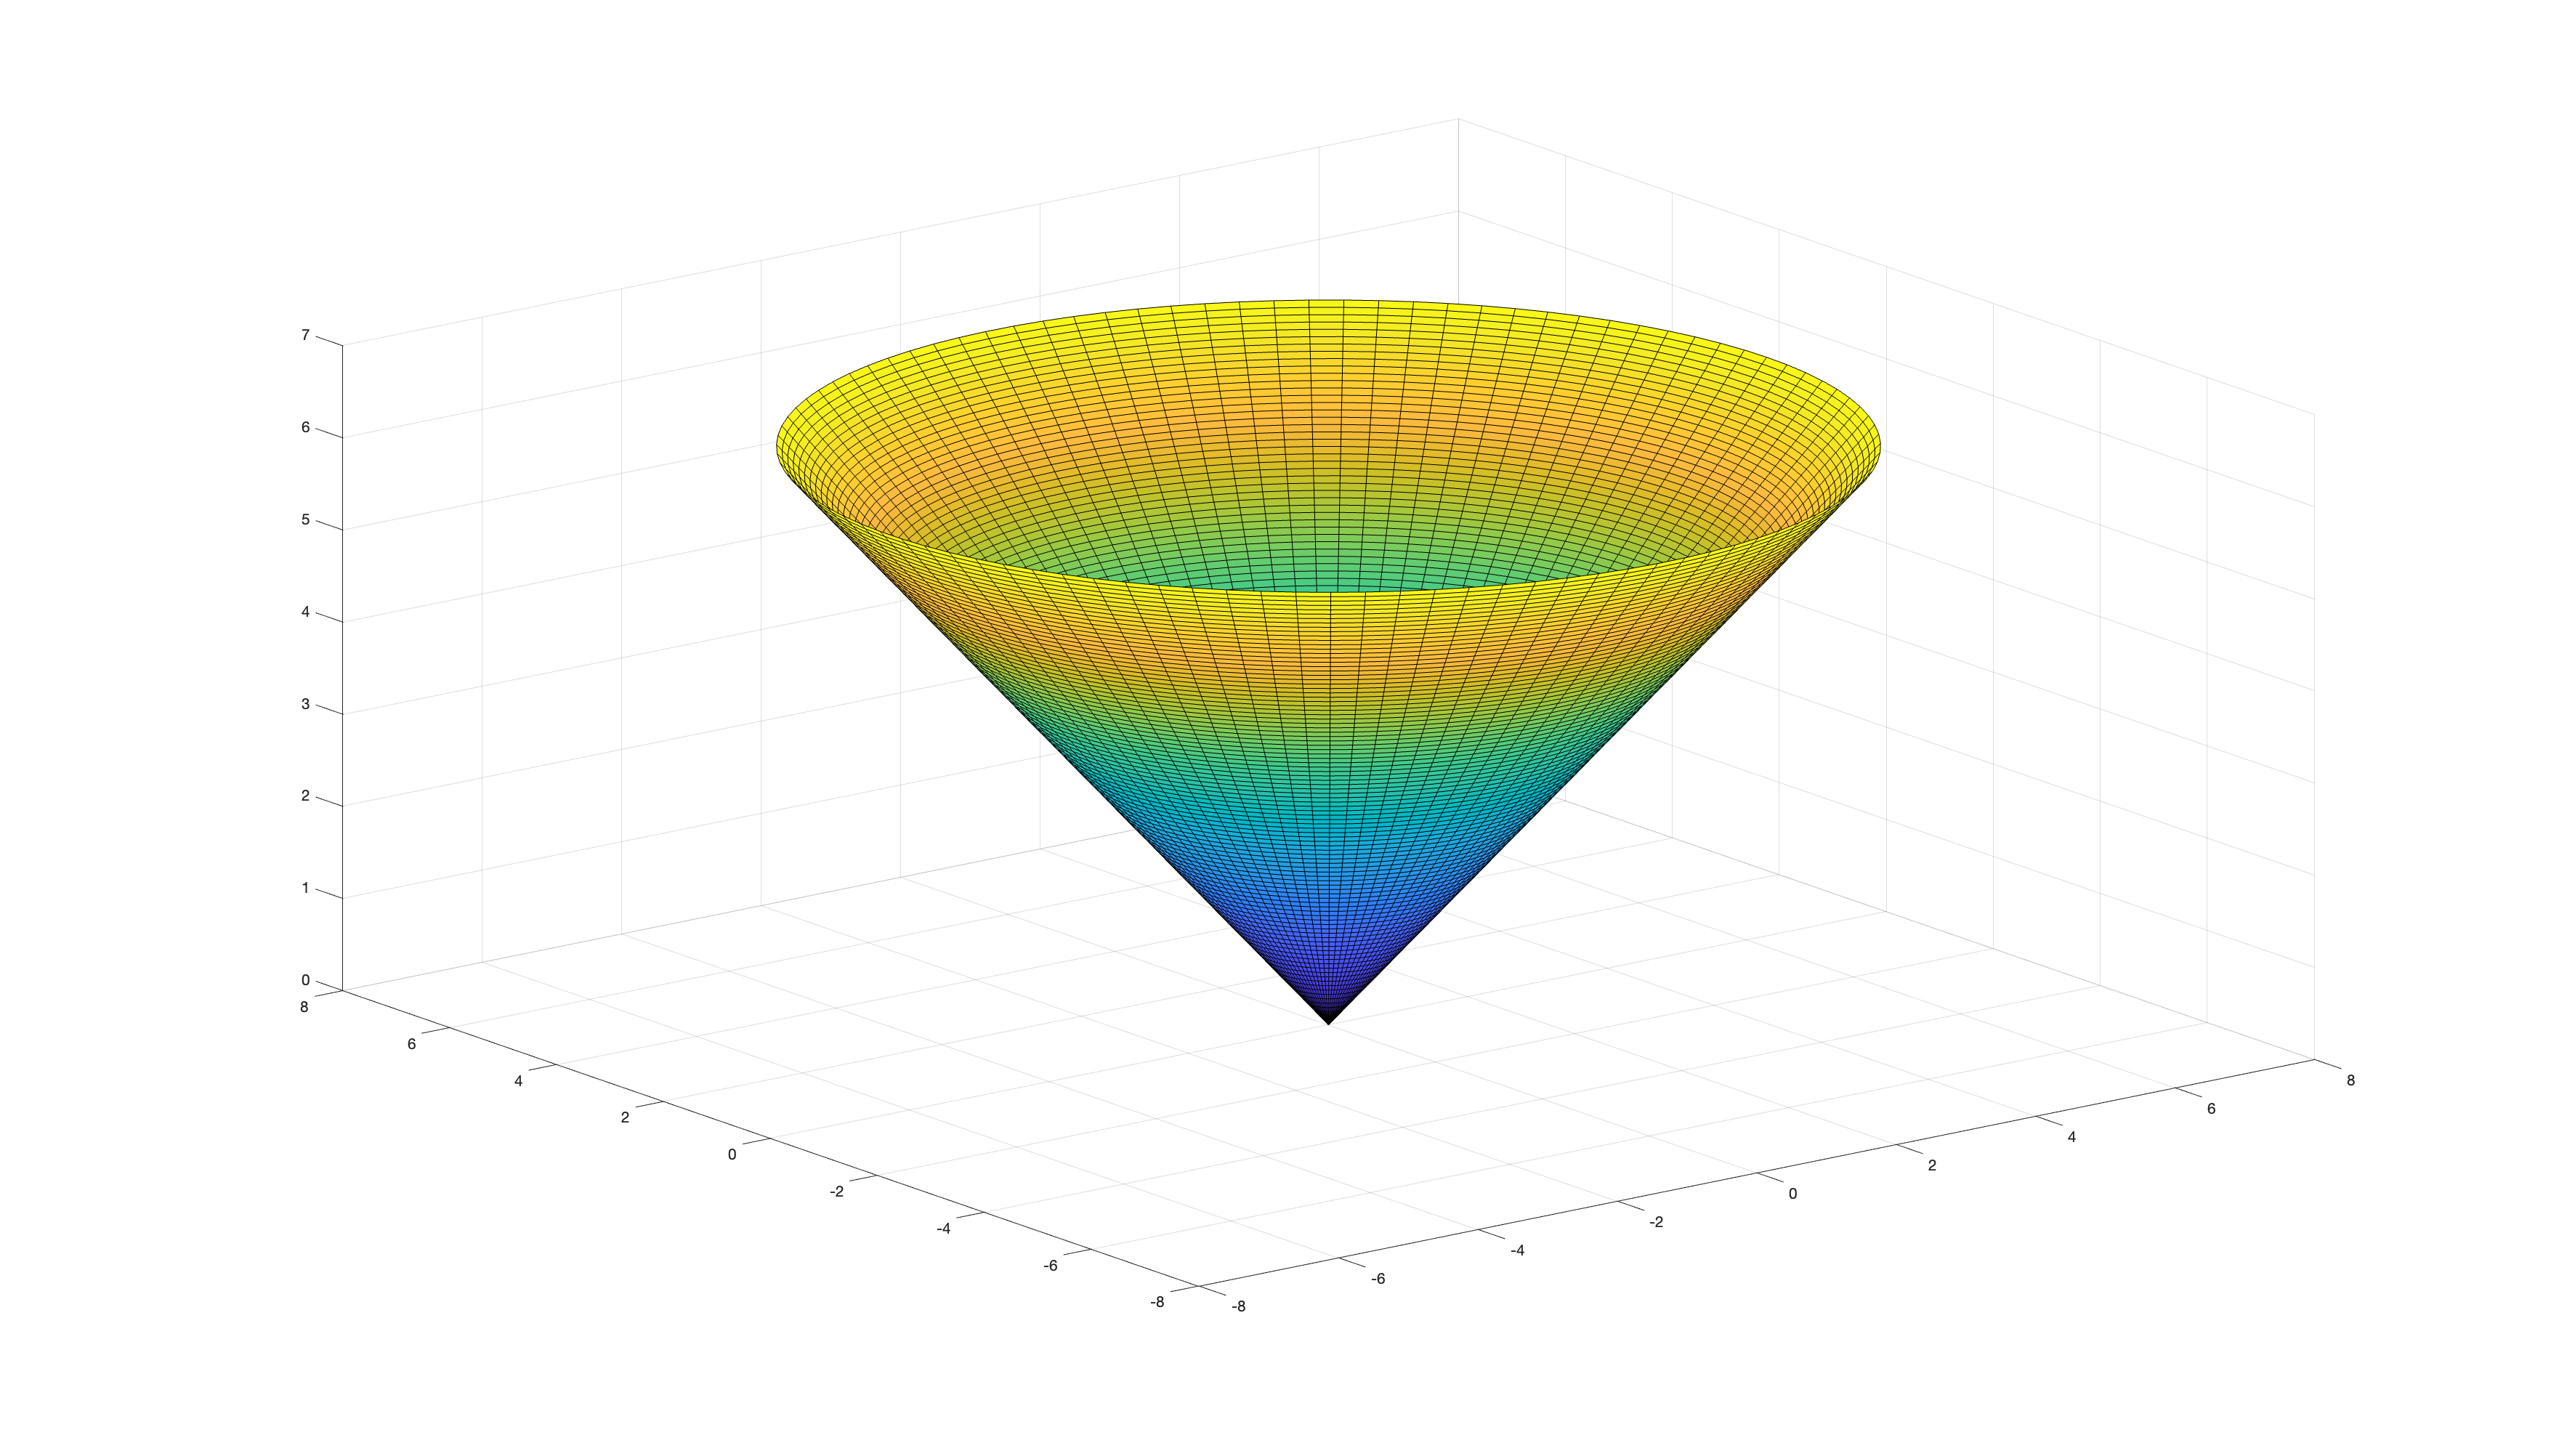
\includegraphics[width=8cm]{img/finiti/cono.eps}
			\caption{Rappresentazione grafica della conica}
			\label{fig:conica}
		\end{figure}
		\begin{equation*}
			\nabla f=0
			\begin{cases}
				z_x=\frac{x}{\sqrt{x^2+y^2}}\\
				z_y=\frac{y}{\sqrt{x^2+y^2}}
			\end{cases}\begin{cases}
					x=0\\
					y=0
			\end{cases} 
		\end{equation*}
		  \begin{nota}
			  sarebbe (0,0) ma il dominio delle derivate $x^2+y^2>0$ cioè
			  $\forall(x,y)\in R^2-\{0,0\}$ in (0,0) non è derivabile.
		  \end{nota}
		  Sappiamo\footnote{si vede geometricamente} che in (0,0) c'è un
		  {\color{red}minimo assoluto}
	  \item $z=x^4 +y^4$
		  \begin{equation*}
			\begin{cases}
				z_x=4x^3=0\\
				z_y=
			\end{cases}\begin{cases}
					x=0\\
					y=0
			\end{cases} \text{ in (0,0) può esserci Max/Min relativo}
		  \end{equation*}
		  \begin{equation*}
			  \begin{matrix}
				det H=\begin{vmatrix}
					0 & 0\\
					0 & 0
				\end{vmatrix} = 0 & \begin{matrix}
					f_{xx}(0,0)=12x^2|_{0,0}=0\\
					f_{xx}(0,0)= 0\\
					f_{yy}(0,0)=12y^2|_{0,0}=0
				  \end{matrix}
			  \end{matrix}
		  \end{equation*}
		  $det H=0 \to$ non so se in (0,0) c'è un massimo o un minimo
		  relativo.\\
		  Per definire se esiste un massimo o un minimo relativo uso:
		  \begin{equation*}
			  \begin{matrix}
				  \min f(x_0,y_0)\leq f(x,y) & 0\leq x^4+y^4 & x^4+y^4\geq 0 &
				  \text{ \underline{SI} $\forall(x,y)$ risulta da
				  $x^4+y^4\geq 0 (0,0)\min$}\\
				  \max f(x_0,y_0)\geq f(x,y) & 0\geq x^4+y^4 & x^4+y^4\leq 0 &
				  \text{ \underline{NO}}
			  \end{matrix}
		  \end{equation*}
  \end{enumerate}
\end{esempio}
\subsection{Ricerca del massimo e del minimo assoluti}
Condizioni sufficienti per l'essistenza del Massimo e del minimo assoluto
\subsubsection{Teorema di Weierstrass}
\begin{teorema}
	Sia f(x,y) definita in D, i continua in D chiuso e limitato, allora il
	minimo e massimo assoluto in D.
	\begin{multicols}{2}
		\paragraph{Ipotesi:}
		\begin{equation*}
			f\in C^0_D
		\end{equation*}
		D chiuso e limitato
		\paragraph{Tesi:}
		$\exists\min$ con $m=f(x_1,y_1), M=f(x_2,y_2)$ tale che $m\leq
		f(x,y)\leq M$
	\end{multicols}
	\paragraph{Ricerca dei punti di Massimo e minimo assoluti:}
	\begin{itemize}
		\item nei punti di massimo o minimo relativo;
		\item nei punti di non derivabilità;
		\item nei punti di frontiera.
	\end{itemize}
	Vanno ricercati quindi nei seguenti modi:
	\begin{enumerate}
		\item $\nabla f=0$ dove il gradiente si annulla;
		\item $\exists \nabla f$ dove il gradiente non esite;
		\item sulla FD sulla frontiera.
	\end{enumerate}
\end{teorema}
\subsubsection{Studio sulla frontiera}
Sia $\xi$ una superficie definita in un insieme D e sia FD la mia frontiera\\
La frontiera FD è una curva\footnote{o insieme di curve} e suoi punti linitano
l'iperbole $\xi$.\\
Possiamo definire la frontiera in forma parametrica
\begin{equation*}
	FD:\begin{cases}
		x=x(t)\\
		y=y(t)
	\end{cases} t\in [a,b] \mathds{R}\to \mathds{R}^2
\end{equation*}
Calcolo la funzione $f(x,y)$ sui punti della frontiera
\begin{equation}
	f(x,y)\to F(t)=f(x(t),y(t))\text{ funzione di 1 variabile}
\end{equation}
studio del massimo e minimo per $F(t)=0\begin{cases}
	F^{\prime\prime}>0 \min\\
	F^{\prime\prime}<0 \max
\end{cases}$\\
Calcolo i valori della funzione nei punti di Massimo/minimo e li confronto con
i valori Massimo/minimo relativi nel dominio e i valori nei punti di non
derivabilità. La frontiera può anche essere in forma cartesiana
\begin{equation}
	\begin{matrix}
		y=y(x) & a\leq x\leq b
	\end{matrix}
\end{equation}
Calcolo la funzione nei punti della frontiera e procedo come visto prima
$f(x,y)\to F(t)=f(x(t),y(t))$
\begin{esempio}
	Determinare il massimo e il mino assoluto di $f(x,y)=
	1+2x^2+\sqrt{x^2+y^2}$ in $D:\{x^2+y^2\leq \Delta\}$
	\begin{enumerate}
		\item $\nabla f=0$
		\item $\nexists \nabla f$
		\item $FD$
	\end{enumerate}
	\begin{enumerate}
		\item $\nabla f(x,y)=0\begin{cases}
				f_x=0\\
				f_y=0
		\end{cases}\begin{cases}
			4x+\frac{x}{\sqrt{x^2+y^2}}\\
			\frac{y}{\sqrt{x^2+y^2}}
		\end{cases}\begin{cases}
			4x+\frac{x}{\abs x}=0\\
			y=0
		\end{cases}$
		\begin{equation*}
			\begin{cases}
				x=0\\
				y=0
			\end{cases}
		\end{equation*}
			$\nabla f=0$ in (0,0) che non è nel C.E. delle derivate parziali
			per cui $\nabla f \neq 0$ $\forall (x,y)\in A$ A dominio $f_x$ e
			$f_y$
		\item $\nexists \nabla f$ le derivate parziali perime sono definite
			$\forall (x,y)\in R^2:x^2+y^2\neq 0$ cioè in $R^2-\{0,0\}$
			\begin{equation*}
				(0,0) \text{ pnto di non derivabilità } f(0,0)=1
			\end{equation*}
		\item FD
			\begin{equation*}
				\begin{matrix}
					D:\{x^2+y^2\leq 4\} & FD: x^2+y^2=4\\
					& \begin{cases}
						x=2\cos t \\
						y=2\sin t
					\end{cases} t\in [0;2\pi]
				\end{matrix}
			\end{equation*}
			Calcolo $f(x,y)$ sui punti di frontiera
			\begin{equation*}
				f(x,y)=F(t)=1+2(2\cos t)^2+\sqrt{(2\cos t)^2+(2\sin t)^2} =
				1+8\cos^2t+2 = 3+8\cos^2t
			\end{equation*}
			Calcolo $F(t)$ agli estremi $t\in[0;2\pi]$ $F(0)=3+8=11$
			$F(2\pi)=3+8=11$\\
			Studio del massimo e del minimo di $F(t)$
			\begin{equation*}
				\begin{matrix}
					F^\prime(t)=0 & 16\cos t(\sin t)=-16\sin t\cos t =0 & t=0&
					t=\pi & t=\frac{\pi}{2}t=\frac{3}{2} \pi
				\end{matrix}
			\end{equation*}
			\begin{equation*}
				F^{\prime\prime}(t)=16(\cos t \cos t -\sin t \sin t) =16(\sin^2
				t- \cos^2 t)
			\end{equation*}
			\begin{equation*}
				\begin{matrix}
					\text{Ottenuti mettendo a F(t) e valori}\\
					\text{dove ci dovrebbero essere un}\\
					\text{massimo e un minimo}
				\end{matrix} \begin{cases}
					F^{\prime\prime}(\pi)=16(-1)=-16<0\text{ }\max\text{ su FD
					}&
					F(\pi) =3+8=11\\
					F^{\prime\prime}(\frac{\pi}{2})=16(-1)=-16>0\text{
					}\min\text{ su
					FD }& F(\frac{\pi}{2}) =3\\
					F^{\prime\prime}(\frac{3\pi}{2})=16(-1)=-16<0\text{
					}\min\text{ su
					FD }& F(\frac{3\pi}{2}) =3
				\end{cases}
			\end{equation*}
	\end{enumerate}
	Ho ottenuto i sequenti valori
	\begin{equation*}
		\begin{matrix}
			1.\text{ }(x,y) \equiv (0,0) & \text{il }\min \text{ è 1 e viene assunto in
			(0,0)} \\
			11.\text{ }t=0,\pi,2\pi & \text{il } \max \text{ è 11 e viene
			assunti in }&
			\begin{cases}
				x=2\cos 0\\
				y=2\sin 0
			\end{cases}\\
			3.\text{ }t=\frac{\pi}{2}, \frac{3}{2}\pi & \begin{cases}
				x=2\cos \pi \\
				y=2\sin \pi
			\end{cases} & (-2,0) & \begin{cases}
				x=2\cos 2\pi \\
				y=2\sin 2\pi
			\end{cases} & (2,0)
		\end{matrix}
	\end{equation*}
\end{esempio}
\subsection{Metodo dei moltiplicatori di di Lagrange}
Nel caso in cui $g(x,y)=0$ non definisca una funzione implicata, per trovare i
massimi e minimi vincolati si introduce una funzione ausiliaria, detta
\underline{\color{red}lagrangiana}, così definita:
\begin{equation}
	F(x,y,\lambda)=f(x,y)+\lambda g(x,y)
\end{equation}
$F(x,y,\lambda)$ è combinazione lineare delle funzioni $f(x,y)$ E $g(x,y)$ --
Il parametro $\lambda$ prende il nome di {\color{red}Moltiplicatore di
Lagrange}. I punti di massimo vincolati sono quelli in cui il gradiente di
$F(x,y,z)$ si annulla ovvero\dots
\begin{equation}
	\nabla F_{(x,y,z)}=0 \begin{cases}
		F_x=fx(x,y)+\lambda g_x(x,y)\\
		F_y=fx(x,y)+\lambda g_y(x,y)\\
		F_\lambda=g(x,y)=0
	\end{cases}
\end{equation}
Si risolve questo sistema di tre equazioni in tre variabili e il valore massimo
della funzione è calcolata nei punti soluzioni è il massimo calcolato e il
valore minimo della funzione calcolata nei punti soluzione è il massimo
vincolato.

\chapter{Integrali Doppi e tripli}
\section{Domini normali (semplici)}
\begin{defi}
	I domini delle funzioni a più variabili possono presentare una forma di
	regolarità per cui è possibile delimitare la regione da intervalli e grafici
	di funzione. Si parla quindi di dominio semplice o normale rispetto alla
	variabile delimitabile da un intervallo. La normalità di un dominio è molto
	importante in molte definizioni di integrale multiplo e della sua
	risoluzione tramite le formule di riduzione. Inoltre la presenza di un
	dominio regolare permette ulteriori teoremi e formule d'integrazione, come
	le formule di Gauss-Green, il teorema della divergenza e il teorema del
	rotore.
\end{defi}
\subsection{Dominio normale rispetto all'asse $x$}
Il dominio A si definisce {\color{red} normale} rispetto all'asse $x$ se è così
definito:
\begin{equation}
	A=\begin{cases}
		a\leq x\leq b & x \text{ valria in un intervallo}\\
		g_1(x)\leq y\leq g_2(x) & y \text{ varia tra due funzioni di }x
	\end{cases}
\end{equation}
\begin{esempio}
\begin{equation*}
	D=\begin{cases}
		0\leq x\leq 1\\
		x^2\leq y\leq x
	\end{cases}
\end{equation*}
\end{esempio}
Il dominio $B$ si definisce {\color{red} normale} rispetto all'asse $x$ se è così
definito:
\begin{equation}
	A=\begin{cases}
		c\leq y\leq d & y \text{ valria in un intervallo}\\
		h_1(y)\leq x\leq h_2(y) & x \text{ varia tra due funzioni di }y
	\end{cases}
\end{equation}
\begin{esempio}
\begin{equation*}
	D=\begin{cases}
		0\leq y\leq 1\\
		y< x< \sqrt{y}
	\end{cases}
\end{equation*}
\end{esempio}
\subsection{Domini Polarmente normale}
Il dominio C si definisce polarmente normale se è costantemente definito:
\begin{equation}
	C=\begin{cases}
		\theta_1\leq \theta\leq \theta_2 \\
		\varphi_1(\theta)\leq \varphi(\theta)\leq \varphi_2(\theta)
	\end{cases}
\end{equation}
\begin{esempio}
  \begin{equation}
    (x-1)^2+y^2\leq 1
  \end{equation}
  l'angolo varia tra 0 e $\frac{\pi}{2}$, il segmento $\varphi$ dipende dall'angolo
  \begin{equation*}
    \begin{matrix}
      \theta=0\text{ è } \max \varphi=2 \\
      \theta=\frac{\pi}{2} \text{ è } \min \varphi=0 \\
      \varphi=2\cos \theta
      \begin{cases}
        0\leq \theta \leq \frac{\pi}{2}\\
        0\leq \varphi\leq 2\cos \theta
      \end{cases}
    \end{matrix}
  \end{equation*}
  corona circolare $\varphi=r$ $\varphi=R$
  \begin{equation*}
    \begin{cases}
      0\leq \theta \leq \frac{\pi}{2}\\
      r\leq \varphi\leq R
    \end{cases}
  \end{equation*}
\end{esempio}
\subsection{Definizione di integrale doppio}
\begin{defi}
  Sia f(x,y) una funzione limitata nel rettangolo $R=[a,b]x[c,d]$, coordinata in $[a,b]$ e
  di seconda coordinata in $[c,d]$
  Deconpongo regolarmante gli intervalli $[a,b]$ e $[c,d]$,
  \begin{equation*}
    \begin{matrix}
        \text{decomponendo }[a,b]\text{ si ha} & D_1=\{x_0=a,x_1,x_2,\dots,x_n=b\}\\ 
        \text{decomponendo }[c,d]\text{ si ha} & D_1=\{y_0=a,y_1,y_2,\dots,y_n=d\}
    \end{matrix}
  \end{equation*}
  Il prodotto cartesiano $D=D_1*D_2$ è una semidivisione del rettangolo R
  \begin{figure}[ht]
    \centering
    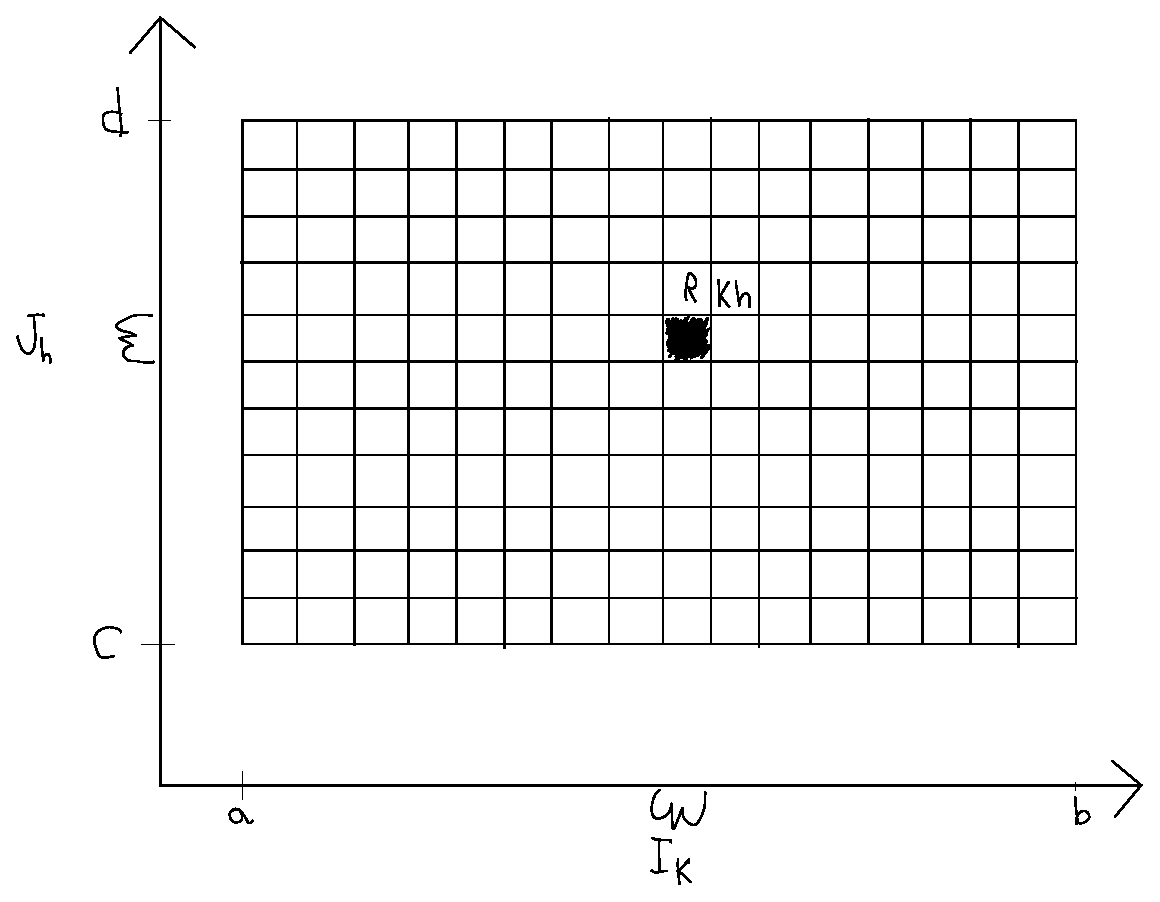
\includegraphics[width=8cm]{img/finiti/graficodecomposizioneR.eps}
    \caption{Decomposizione del rettangolo R}
  \end{figure}
  \begin{equation*}
    \begin{matrix}
        I_k=[x_{k-1},x_k] \text{ in } D_1 (k=1,\dots,n)\\
        J_h=[y_{h-1},y_h] \text{ in } D_2 (h=1,\dots,n)
    \end{matrix}
  \end{equation*}
  Il prodotto cartesiano $I_k*J_h$ individua il generico subrettangolo $R_{kh}$ della semidivisione.\\
  Prendo un generico punto del subrettangolo $R_{kh}(x_k,y_h)$ e faccio il seguente prodotto:
  \begin{equation*}
    f(x_k,y_h)*mis R_{kh} \text{ con } misR_{kh} = misI_k * misJ_h \text{ area del subrettangolo}
  \end{equation*}
  Con l'integrale doppio consudero il volume del parallelepipedo.\\
  Geometricamente considera il pettangolo $R_{kh}$ e la parte di superficie $f(x,y)$ che vi si
  presenta il prodotto $f(x_i,y_n)*mis R_{kh}$ è il volume del parallelepipedo di base $R_{kh}$
  e altezza $f(x_k,y_h)$.
\end{defi}
\section{Somme di Riemann}
Definisco le somme di Riemann $\displaystyle\sum^{k=m\text{ } h=n}_{k=h=1}f(x_k,y_h)*R_{kh}$ ciò
rappresenta la somma di tutti i volumi dei parallelepipedi di base $R_{kh}$ e altezza $f(x_k,y_h)$
che si possono ottenere nel rettangolo $R$.\\
Infittisco le decomposizioni $D_1$ e $D_2(m\to \infty;n\to\infty)$, ottenendo così un numero sempre
maggiore di subrettangoli di ampiezza via via minore.
\begin{equation}
  mis R_{kn}=misI_k*misI_n=\frac{b-a}{m} * \frac{d-c}{n}\to 0 \text{ per }  m,n \to \infty
\end{equation}
Con l'infittirsi della decomposizione, aumenta la precisione con cui ciascun parallelepipedo
approssima il volume sotto al grafico delle funzione in ogni $R_{kh}$.\\
Al limite, le somme di Riemann daranno il volume sotto al grafico della funzione in un certo
rettangolo (in generale dominio).\\
Se esiste finito $\lim\limits_{n\to \infty\text{ } m\to \infty}\displaystyle\sum_{h=k=1}^{k=m\text{ }h=n}f(x_k.y_n)*misR_{kh}$ tale limite è definito \underline{\color{red} ingrale doppio} di f(x,y) nel
dominio $R=[a,b]*[c,d]$
\begin{equation}
  \iint_R f(x,y)dxdy=\lim\limits_{n\to \infty\text{ } m\to \infty}\displaystyle\sum_{h=k=1}^{k=m\text{ }h=n}f(x_k.y_n)*misR_{kh}
\end{equation}
\paragraph{Somme superiori e somme inferiori}
\begin{defi}
  È possibile definire l'integrale doppio anche con le somme superiori e le somme inferiori
  \begin{equation*}
    \text{Somme inferiori } s(f,R) = \displaystyle\sum inf_{R_{kh}}f(x_k.y_n)*misR_{kh}
  \end{equation*}
  prendo il minimo valore che la funzione assume nel subrettangolo $R_{kh}$ e lo moltiplico per
  l'area di tale subrettangolo. Sommando ottengo un parallelepipedo, il cui volume approssima
  per difetto individuato dalla funzione. 
  \begin{equation*}
    \text{Somme superiori } s(f,R) = \displaystyle\sum sup_{R_{kh}}f(x_k.y_n)*misR_{kh}
  \end{equation*}
  prendo il massimo valore che la funzione assume nel subrettangolo $R_{kh}$ e lo moltiplico per
  l'area di tale subrettangolo. Sommando ottengo un parallelepipedo, il cui volume approssima per
  eccesso quello individuato dalla funzione all'infittirsi della decomposizione le somme inferiori
  crescono, le somme superiori decrescono. Le somme superiori e le somme inferiori convergono ad
  uno stesso valore, detto {\color{red}integrale doppio}\footnote{è il valore sotto al grafico
    della funzione}
  \begin{equation*}
    \lim s=\lim S=\iint_R f(x,y)dxdy
  \end{equation*}
\end{defi}
\clearpage
\subsection{Proprietà dell'integrale doppio}
\begin{equation*}
  \begin{matrix}
  \text{Linearità } \begin{cases}
                      1) \iint_D [f_1(x,y)+f_2(x,y)]dxdy=\iint_Df_1(x,y)dx*dy+\iint_Df_2(x,y)dx*dy\\
                      2) \iint_D \alpha f_1(x,y)dxdy=\alpha\iint_Df_2(x,y)dx*dy
                    \end{cases}\\
    \text{Assitività } 3)\text{ Sia } D=D_1\cup D_2 \iint_Df(x,y)dxdy=\iint_{D_1}f(x,y)dx*dy +\iint_{D_2}f(x,y)dx*dy\\
    \text{Monotonia } \begin{cases}
                        4) \text{ Sia } f(x,y)\leq g(x,y)\text{ } \forall (x,y) \in D\\
                        \text{ }\iint_Df(x,y)dxdy \leq \iint_Dg(x,y)dx*dy\\
                        5) \text{ Sia } D_1 \subset D\\
                        \text{ } \iint_{D_1}f(x,y)dxdy < \iint_Df(x,y)dx*dy \\
                        6) \abs{\iint_Df(x,y)dxdy} \leq \iint_D\abs{f(x,y)}dx*dy
                      \end{cases}
  \end{matrix}
\end{equation*} 

\subsection{Formula di riduzione}
\begin{itemize}
\item Sia $A\subset R^2$ un dominio normale rispetto all'asse x
  \begin{equation*}
    A=\begin{cases}
        a\leq x\leq b\\
        g_1(x)\leq y\leq g_2(x)
      \end{cases}
  \end{equation*}
    Allora $\iint_A f(x,y) dxdy=\int_a^bdx \left(\int_{g_1(x)}^{g_2(x)}f(x,y)dy\right)$\\
    calcolo prima $\int_{g_1(x)}^{g_2(x)}f(x,y)dy$ che è una funzione della sola $x$ $\not{o}(x)$
    \begin{equation*}
      \text{per calcolo } \int^b_a \not{o} (x) dx
    \end{equation*}
  \item Dominio polarmente normale\\
    Effettua un cambio di coordinate, passando dalle coordinate cartesiane a quelle polari
    \begin{equation*}
      \text{L'integrale doppio è } \iint_Df(x,y)dxdy
    \end{equation*}
    Passando alle coordinate polari
    \begin{equation*}
      \begin{matrix}
        \text{del dominio } D(x,y) \text{ passerò al dominio } D^\prime (\varphi, \theta) \\
        \text{della funzione } f(x,y) \text{ passerò al dominio } f (\varphi, \theta)
      \end{matrix} \begin{cases}
                       x=\varphi\cos\theta\\
                     y=\varphi\sin\theta
                   \end{cases}
                   \varphi=\sqrt{x^2+y^2} 
   \end{equation*}
   e da differenziali $dxdy$ passerò ai differenziali $d\varphi d\theta$. \\
   Si dimostra che nel passaggio ad altre coordinate il differenziale è $\abs{j} d\varphi d\theta$,
   dove $\abs j$ è il determinante della {\color{red} matrice Jacobiana} che contiene le derivate
   parziale prime
   \begin{equation}
     \abs{J}=\begin{vmatrix}
               x_\varphi & x_\theta\\
               y_\varphi & y_\theta
             \end{vmatrix}
             \to \abs{J}=\begin{vmatrix}
                           \cos \theta & -\varphi \sin \theta\\
                           \sin \theta & \varphi \cos \theta
                         \end{vmatrix}
                         =\varphi\cos^2\theta+\varphi \sin^2\theta =\varphi
   \end{equation} 
   Per cui passando da $dxdy$ alle coordinate polari avrò $\varphi d\varphi d\theta$ così
   l'integrale doppio diventa:
   \begin{equation*}
     \iint_Df(x,y)dxdy=\iint_{D^\prime}f(\varphi,\theta)\varphi d\varphi d\theta
   \end{equation*}
\end{itemize}
\clearpage
\subsubsection{Esempi di domini polarmente normali}
\begin{figure}[ht]
  \centering
  \includegraphics[width=14cm]{img/finiti/esdompolnorm.eps}
  \caption{Esempi di domini polarmente normali}
\end{figure}
\subsection{Baricentro di un dominio normale}
\begin{defi}
  Sia D un demonio normale del piano. Si definisce {\color{red}baricentro del dominio} D il punto di
  coordinate $(x_0,y_0)$ tale che:
  \begin{equation*}
    \begin{matrix}
      x_0=\frac{1}{mis D} \iint_D xdxdy & y_0=\frac{1}{mis D} \iint_D ydxdy
    \end{matrix}
  \end{equation*}
  $mis D:$ misura ({\tt area}) del dominio $D$.
\end{defi}
\begin{esempio}
  calcolare il baricertro del dominio $D=\begin{cases}
                                           0\leq x\leq 2\\
                                           0\leq y\leq 1
                                         \end{cases}$
  \begin{equation*}
    mis D=A_{rettangolo}=2*1=2
  \end{equation*}
  \begin{figure}[ht]
    \centering
    \includegraphics[width=6cm]{img/finiti/baricentrodiundominionormale.eps}
    \caption{Baricentro di un dominio normale}
  \end{figure}
  \begin{equation*}
    \begin{matrix}
      x_0=\frac{1}{mis D}\iint_D xdxdy=\frac{1}{2}\int_0^2dx\int_0^1xdy=\frac{1}{2}\int^2_0dx\abs{xy}_0^1= \frac{1}{2}\int_0^2xdx=\frac{1}{2}\abs{\frac{x^2}{2}}_0^2=\frac{1}{\not{2}}\not{2}=1\\
      y_0=\frac{1}{mis D}\iint_D ydxdy=\frac{1}{2}\int_0^2dx\int_0^1ydy=\frac{1}{2}\int_0^2dx\left|\frac{y^2}{2}\right|^1_0=\frac{1}{2}\int^2_0\frac{1}{2}dx=\frac{1}{4}\left|x\right|=\frac{1}{2}
    \end{matrix}
  \end{equation*}
  \clearpage
   \begin{center}
            \fbox
            {
            \begin{minipage}{0.85\textwidth}
		Calocolare il baricentro del dominio $D=\begin{cases}
                                                          0\leq \theta \leq \frac{\pi}{2}\\
                                                          0\leq y \leq \sqrt{1-x^2}
                                                          \end{cases}$
              \begin{multicols}{2}
                \includegraphics[width=6cm]{img/finiti/baricentrodiundominionormale2.eps}\\
                \begin{equation*}
                  \begin{matrix}
                    D=\begin{cases}
                      0\leq \theta\leq\frac{\pi}{2}\\
                      0\leq \varphi\leq 1
                    \end{cases} & mis D=\frac{\pi}{4}
                  \end{matrix}
                \end{equation*}
              \end{multicols}
              \begin{equation*}
                \begin{matrix}
                  x_0= \frac{1}{mis D}\iint_D xdxdy=\frac{4}{\pi}
                  \int^{\frac{\pi}{2}}_0d\theta\int_0^1
                  \varphi^2\cos \theta d\theta = \frac{4}{\pi} \int_0^{\frac{\pi}{2}}d\theta \left|
                  \frac{\varphi^3}{3}\cos\theta\right|_0^1\\=\frac{4}{\pi}\int_0^{\frac{\pi}{2}}
                  \frac{1}{3} \cos \theta d\theta = \frac{4}{3}\pi \left|\sin
                  \theta\right|^{\frac{\pi}{2}}_0=\frac{4}{3}\pi\\
                  y_0=\frac{1}{mis D}\iint_D xdxdy=\frac{4}{\pi}
                  \int^{\frac{\pi}{2}}_0d\theta\int_0^1
                  \varphi^2\sin \theta d\theta = \frac{4}{\pi} \int_0^{\frac{\pi}{2}}d\theta \left|
                  \frac{\varphi^3}{3}\sin\theta\right|_0^1\\
                  =\frac{4}{\pi}\int_0^{\frac{\pi}{2}}\frac{1}{3}\sin\theta d\theta =\frac{4}{\pi}*
                  \frac{1}{3}\left|-\cos\theta \right|^{\frac{\pi}{2}}_0=\frac{4}{3}\pi
                \end{matrix}
              \end{equation*} 
            \end{minipage}
            }
  \end{center}
\end{esempio}
\subsection{Domini normali in $R^3$}
\begin{defi}
Il dominio $V$ definisce normale rispetto al piano $xy$ se si può così descrivere:
\begin{equation*}
  \begin{matrix}
    \begin{cases}
      (x,y)\in D & \text{normale}\\
      \alpha(x,y) & \leq z\leq \beta (x,y)
    \end{cases}& \begin{matrix}
                   (x,y) \text{ appartengono ad un dominio normale di } R^2\\
                   z \text{ è compresa tra funzioni di } x \text{ e } y 
                 \end{matrix}
  \end{matrix}
\end{equation*}
$\forall (x,y)\in D$ incontro prma la superficie minorante e per la superficie maggiorante.
\end{defi}
\section{Integrali tripli}
\begin{defi}
  Sia $f(x,y,z)$ una funzione limitata in un insieme $V$, considero il parallelepipedo
  \begin{multicols}{2}
    \begin{equation*}
      V=[a,b]*[c,d]*[e,f]
    \end{equation*}
    Decompongo regolarmente $[a,b],[c,d],[e,f]$\\
    rispettivametne in $n,m e k$\\
    intervalli $I_n=[x_0=a,\dots,x_n=b]$,
    \begin{equation*}
      l_m=[y_0=c,\dots,y_m=d],\text{ } l_k=[z_0=e,\dots,z_k=f]
    \end{equation*}
    \includegraphics[width=4cm]{img/finiti/rettangolo.eps}
  \end{multicols}
  Il prodotto cartesiano $I_n*I_n*I_k$ individua il generico subparallelepipedo $V_{n,m,k}$.
\end{defi}
\clearpage
Definisco le somme di Riemann: $\sum f(x,y,z)*misV_{n,m,k}$\footnote{$misV_{n,m,k}$: misura il
  volume del parallelepipedo}\\
All'infittirsi delle decomposizioni le somme di Riemann convergono ad uno stezzo valore, tale
valore è definito {\color{red}integrale triplo} di $f(x,y,z)$ in $V$
\begin{equation*}
  \lim_{m\to \infty\text{ } n \to \infty \text{ } k\to \infty}\sum f(x,y,z) misV_{n,m,k}=\iiint_V f(x,y,z)dxdydz
\end{equation*}
Oppure, definisco le somme inferiore e le somme superiori
\begin{equation*}
  \begin{matrix}
    \text{Somme inferiori} &\sum misV_{n,m,k}*\min_{V_{n,m,k}}f(x,y,z)\\
    \text{Somme superiori} &\sum misV_{n,m,k}*\max_{V_{n,m,k}}f(x,y,z)
  \end{matrix}
\end{equation*}
All'infittirsi della decomposizione le somme inferiori crescono mentre le somme superiori
decrescono. Se convergono ad una stesso valore, tale valore è definito {\color{red}integrale triplo}
di $f(x,y,z)$ in $V$
\begin{equation*}
  \lim s(f,V)= \lim S(f,V)= \iint_V f(x,y,z) dxdydz
\end{equation*}
\subsection{Formule di riduzione per gli integrali tripli}
Sia $g(x,y)$ integrabile in un dominio normale $V$
\begin{equation*}
  \begin{matrix}
    V=\begin{cases}
        \alpha (x,y) \leq z\leq \beta (x,y)\\
        (x,y)\in D
      \end{cases} & \iiint_V f(x,y,z) dxdydz = \iint_D dxdy \displaystyle\int_{a(x,y)}^{\beta (x,y)} f(x,y,z)dz
  \end{matrix}
\end{equation*}
Se il dominio $D$ è normale rispetto all'asse $x$
\begin{equation*}
	V=\begin{cases}
		a\leq x\leq b\\
		g_1(x)\leq y\leq g_2(x)\\
		\alpha (x,y) \leq z \leq \beta (x,y)
	\end{cases} \iiint_V f(x,y,z) dxdydz = \int_\theta^\theta dx
	\int_{f_1(x)}^{f_2(x)}dy\int_{\alpha(x,y)}^{\beta(x,y)}f(x,y,z)dz
\end{equation*}
Se il dominio $D$ è normale rispetto all'asse $y$
\begin{equation*}
	V=\begin{cases}
		c\leq y \leq d\\
		h_1(y)\leq x \leq h_2(y)\\
		\alpha (x,y) \leq z \leq \beta(x,y)
	\end{cases} \iiint_V f(x,y,z) dxdydz = \int_c^d dy
	\int_{h_1(y)}^{h_2(y)}\int_{a(x,y)}^{\beta(x,y)} f(x,y,z) dz
\end{equation*}
Se il dominio $D$ è polarmente normale
\begin{equation*}
	V=\begin{cases}
		\theta_1\leq \theta \leq \theta_2\\
		\varphi_1(\theta)\leq \varphi \leq \varphi_2(\theta)\\
		\alpha (\varphi,\theta)\leq z \leq \beta(\varphi,\theta)
	\end{cases} \iiint_V f(x,y,z)dxdydz=\int_{\theta_1}^{\theta_2}d\theta
	\int^{\varphi_2(\theta)}_{\varphi_1(\theta)} \varphi d \varphi
	\int^{\beta(\varphi, \theta)}_{\alpha (\varphi,\theta)}
	f(\varphi,\theta,z)dz 
\end{equation*}
\begin{equation*}
	\begin{matrix}
		\alpha(x,y)&\to&\alpha (\varphi, \theta)\\
		\beta (x,y)&\to& \beta(\varphi, \theta)\\
		f(x,y,z) &\to & f(\varphi,\theta, z)\\
		dxdydz &\to & pd\theta d\varphi dz
	\end{matrix}
\end{equation*}
\clearpage
\subsection{Significato geometrico degli integrali}
\begin{equation*}
	\begin{matrix}
		\int & \text{area}\\
		\iint & \text{volume}\\
		\iiint & \text{nessun significato geometrico}
	\end{matrix}
\end{equation*}
\subsection{Coordinate polari e coordinate cilindriche}
$(x,y) \to (\varphi,\theta)$
\begin{equation*}
	\begin{matrix}
		\begin{cases}
			x=\varphi \cos \theta\\
			y=\varphi \sin \theta
		\end{cases} & \varphi =\sqrt{x^2+y^2} &det J=\varphi
	\end{matrix}
\end{equation*}
\paragraph{coordinate alindriche}
$(x,y,z)\to (\varphi,\theta,z)$
\begin{equation*}
	\begin{matrix}
		\begin{cases}
			x=\varphi \cos \theta\\
			y=\varphi \sin \theta\\
			z=z
		\end{cases} & \varphi =\sqrt{x^2+y^2+z^2} &det J=\varphi
	\end{matrix}
\end{equation*}
\paragraph{coordinate sferiche}
\begin{equation*}
	\begin{matrix}
		\begin{cases}
			x=\varphi \sin\theta \cos \alpha\\
			y=\varphi \sin \theta \sin \alpha\\
			z=\varphi \cos\theta
		\end{cases} 
	\end{matrix}
\end{equation*}
\subsection{Interazione per fette}
Considera un volume $V$ e lo interseco con un piano $z=k$. Così ottengo una
sezione $S_z$
\begin{equation*}
	z=1-x^2-y^2
\end{equation*}
Al variare di $z$ tra due valori, cioè facendo variare $S_z$ in funzione di $z$
descrivo il volume $V$.
\begin{esempio}
	\begin{equation*}
		\int_{0}^{1} S_zdz
	\end{equation*}
	$S_z$ è un cerchio di raggio $R(z)$ che depende da $z$
	\begin{equation*}
		\begin{matrix}
			z=1-x^2+y^2 & x^2+y^2=1-z\\
			R^2=1-z & R(z)=\sqrt{1-z}
		\end{matrix}
	\end{equation*}
	$S_z=\pi R^2=\pi(1-z)$
	\begin{equation*}
		\iint_T f(x,y,z)dxdydz=\int_0^1\pi(1-z)dz
	\end{equation*}
\end{esempio}
\subsection{Integrali curvilinei}
\subsubsection{Curve in $R^2$ e in $R^3$}
\begin{defi}
	Si definisce {\color{red}curva} una coppia del tipo $(\gamma,\Gamma)$ con
	\begin{equation*}
		\vec{F}(t)=(x(t),y(t),z(t),\dots) \text{ } t\in [a,b]
	\end{equation*}
	si tratta di un'applicazione $R\to R^n$ ad un valore di $t$ associo $n$
	valori\\
	Le curve possono essere:
	\begin{itemize}
		\item In forma cartesiana $\begin{matrix}
				z=f(x,y) &(R^3) \\
				y=f(x) &(R^2)
		\end{matrix} \begin{cases}
			x=t\\
			y=f(t)
		\end{cases}$
		\item In forma polare $\begin{matrix}
			\varphi =\varphi(\theta)&\varphi=2r\cos\theta & 0\leq \theta \leq 2\pi
	\end{matrix}$
		\item In forma parametrica $\begin{cases}
			x=x(t)\\
			y=y(t)\\
			z=z(t)
		\end{cases}$
	\end{itemize}
	Nello spazio una curva è l'intersezione tra due superfici.\\
	Ogni curva ha anche un {\color{red}sostegno}, che è il suo grafico nek
	piano o nello spazio.\\
	Una curva si definisce {\color{red}chiusa} se
	\begin{equation*}
		\begin{matrix}
			\vec{F}(t)=\begin{cases}
				x=x(t)\\
				y=y(t)
			\end{cases} & t\in [a,b]\text{ se } \vec{F}(a)=\vec{F}(b) &
			\begin{matrix}
				x(a)=x(b)\\
				y(a)=y(b)
			\end{matrix}
		\end{matrix}
	\end{equation*}
	\begin{figure}[ht]
		\centering
		\includegraphics[width=13cm]{img/finiti/curva_chiusa_e_aperta.eps}
		\caption{Differenza tra curva chiusa e aperta}
	\end{figure}\\
	Una curva chiusa la {\color{red}frontiera} di un dominio
	\begin{multicols}{2}
		\includegraphics[width=6cm]{img/finiti/dominio.eps}\\
		\begin{equation}
			FD:\begin{cases}
				x=x(t)\\
				y=y(t)
			\end{cases} t\in [a,b]
		\end{equation}
	\end{multicols}
	Una curva si devinisce {\color{red}semplice} se presi due qualunque
	$t_1\neq t_2$ rusylta $\vec{F}(t_1)\neq \vec{F}(t_2)$ cioè 
	\begin{equation*}
		\begin{cases}
			x(t_1)\neq x(t_2)\\
			y(t_1)\neq y(t_2)\\
			z(t_1)\neq z(t_2)
		\end{cases}
	\end{equation*}
	Curva semplice $\gamma \begin{cases}
		x=t\\
		y=\sqrt{t}
	\end{cases} y=\sqrt{x}$ $\gamma \begin{cases}
		x=t\\
		y=t^2
	\end{cases} y=x^2$ Curva non semplice\footnote{$t_1\neq t_2$ ho due stessi
	valori della curva}\\
	Una curva è {\color{red}regolare} se è di classe $c^1$ e le sue derivate
	prime non sono mai nulle contemporaneamente
	\begin{equation*}
		\vec{F}(t)=\begin{cases}
			x=x(t)\\
			y=y(t)\\
			z=z(t)
		\end{cases}
		\begin{matrix}
			\vec{F}(t)\in c^\prime \\
			t\in[a,b]
		\end{matrix}
		r^\prime(t)=(x^\prime,y^\prime,z^\prime(t)\dots)\neq(0,0,0\dots)
	\end{equation*}
	Curva regolare
	\begin{equation*}
		\begin{matrix}
			\gamma z(t)=\begin{cases}
				x=t^3-t\\
				y=t^2-1
			\end{cases} & f\in [-1,1] & z^\prime(t) =\begin{cases}
				x^\prime(t)=3t^2-1\\
				y^\prime(t)=2t
			\end{cases} &\begin{matrix}
				\text{non sono mai nulle}\\
				\text{contemporaneamente}
			\end{matrix}
		\end{matrix}
	\end{equation*}
	\begin{multicols}{2}
		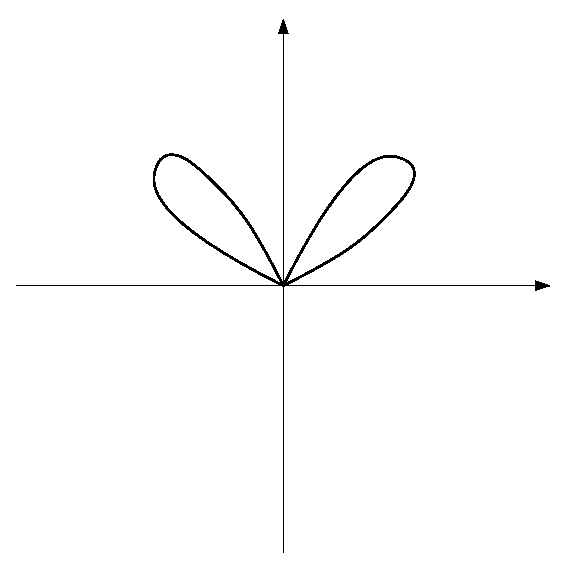
\includegraphics[width=6cm]{img/finiti/curva_regolare.eps}\\
		\begin{equation*}
			r(t)=\begin{cases}
				x=t(1-t^2)^2\\
				y=t^2(1-t^2)
			\end{cases} t\in[-1,1]
		\end{equation*}
	\end{multicols}
	Una curva è {\color{red}regolare a tratti} se è l'unione di curve regolari
	\begin{equation*}
		\gamma r(t)=\begin{cases}
			x=t^3\\
			y=t^2
		\end{cases} t\in[-1,1] \text{ in $x=0$ c'è una cuspide perciò non è regolare $y=\sqrt[3]{x^2}$}
	\end{equation*}
	$r(t)$ può però essere vista come l'unione di che curve regolari
	\begin{equation*}
		\gamma^\prime r (t)=\begin{cases}
			x=t^3\\
			y=t^2
		\end{cases} t\in [-1,0]
	\end{equation*}
	\begin{equation*}
		\gamma^{\prime\prime} r^{\prime\prime}=\begin{cases}
			x=t^3\\
			y=t^2
		\end{cases} t\in [0,1]
	\end{equation*}
	sostegno nel II quadrante
	\begin{equation*}
		\gamma=\gamma^\prime \vee \gamma^{\prime\prime}
	\end{equation*}
\end{defi}
\subsection{Lunghezza di una curva}
\begin{defi}
	Sia la curva $\gamma$ di equazione $\vec{F}(t)$, essa si definisce
	{\color{red}rettificabile} se esiste finito l'estremo superiore della
	poligonale $L(p)$ al variare della decomposizione.
	\begin{equation}
		sup_DL(\Delta)
	\end{equation}
	Suddivido la curva in tanti segmenti che formano la poligonale $L(D)$.
	All'infittirsi la poligonale approssimo sempre seguo la lunghezza della
	curva.\\
	Se la curva $\vec{F}(t)$ è di classe $c^1$ allora essa è
	{\color{red}rettificabile}
	\begin{equation}
		\vec{F}(t)=\begin{cases}
			x=x(t)\\
			y=y(t)\\
			z=z(t)
		\end{cases} t\in [a,b]
	\end{equation}
	e la sua lunghezza vale
	$L=\int_{a}^{b}\sqrt{[x^\prime(t)]^2+[y^\prime(t)]^2 + [z(t)]^2+\dots dt}$
\end{defi}
\subsection{Lunghezza di una curva in forma cartesiana}
Se la curva $\gamma$ nella forma $\begin{cases}
	x=t\\
	y=f(t)
\end{cases} t\in [a,b]$ ha come sostegno il grafico di $y=f(x)$\\
La lunghezza della curva è $L_\gamma=\int_{a}^{b}\sqrt{1+[f^\prime(x)]^2}dx$
\subsection{Lunghezza di una curva polare}
Se le curve è nella forma 
\begin{equation*}
	\begin{cases}
		e=e(\theta)\\
		\theta_1\leq\theta\leq\theta_2
	\end{cases} 
\end{equation*}
La sua lunghezza vale: 
\begin{equation*}
	L_\gamma
	=\int_{\theta_1}^{\theta_2}\sqrt{\varphi^2(\theta)+[\varphi^\prime(\theta)]^2}
	d\theta
\end{equation*}
\section{Ascissa Curvilinea}
È possibile effettuare combiamenti di parametri per descrivere una curva. Fra
tutte le rappresentazioni parametriche di una curva regolare ha particolare
\textbf{importanza} geometrica quella che {\color{red}l'ascissa curvilinea}.
Prendiamo una curva $\gamma$ di $R^2$ e un suo punto $P_0$
\begin{multicols}{2}
	\includegraphics[width=7cm]{img/finiti/ascissa_curvilinea.eps}\\\\\\\\
	Ad ogni punto $P$ della curva associamo un valore $S(P)$ che è uguale
	alla lunguezza dell'arco di curva congiungente $P_0$ e $P$\\
	Così definendo una corrispondenza biurivoca tra i punti della curva e i
	punti di un certo intervallo $[a,b]$, cosiché se $S(p_1)=a$ $S(P_2)=b$ la
	lunqhezza dell'arco congiungente $P_1$ con $P_2$ è $\abs{b-a}$
\end{multicols}
Sia $(\gamma,\vec{r}(t))$ una curva regolare; definiamo \underline{l'ascissa
curvilinea}\footnote{o lunghezza d'arco} come:
\begin{equation*}
	S(t)= \int_{a}^{t}\sqrt{[x^\prime (\uptau)]+[y^\prime(\uptau)]} d\uptau
\end{equation*}
Per il teorema del calcolo integrale
\begin{equation*}
	\begin{matrix}
		S^\prime(t)=\sqrt{[x^\prime(t)]^2+[y^\prime(t)]^2} & S(t) \text{ è
		integrabile}\\
		S^\prime(t)=\frac{ds}{dt} & S:[a,b]\to [0,L]
	\end{matrix}
\end{equation*}
La lunghezza della curva così vale:
\begin{equation}
	L=\int_{a}^{b}\sqrt{[x^\prime(t)]^2+[y^\prime(t)]^2}=\int dS
\end{equation}
\section{Integrale corvilineo}
Prendiamo una funzione f(x,y) definita in un insieme $D$ e una curva $\gamma$
interno a $D$.
\begin{multicols}{2}
	\includegraphics[width=5cm]{img/finiti/integrale_curvilineo.eps}\\
	Calcoliamo la funzione nella curva $\gamma$ e detterminiamo una curva
	$\Gamma$ dello spazio.\\
	L'area delimitata dal cilindro di basi $\gamma$ e $\Gamma$ se $f(x,y)>0$ è
	il valore {\color{red}dell'integrale curvilineo} di $f(x,y)$ esteso a
	$\gamma$.
\end{multicols}
\subsection{Definizione di integrale curvilineo}
Data una curva regolare $(\gamma, \vec{r}(t))$
\begin{equation}
	\begin{cases}
		x=x(t)\\
		y=y(t)\\
		z=z(t)
	\end{cases} t\in [a,b]
\end{equation} 
e una funzione $f(x,y,z)\in \mathds{C}$ -- definita in $D_1$ con la curva
inclusa $D$, si definisce {\color{red}integrale curvilineo} di $f(x,y,z)$
esteso alla curva
\begin{equation*}
	\int_{\gamma} f(x,y,z) ds=
	\int_{a}^{b}f[x(t),y(t),z(t)]*\sqrt{[x^\prime(t)]^2+[y^\prime(t)]^2+[z^\prime(t)]^2}
	dt
\end{equation*}
\subsection{Baricentro di una curva}
Si definisce {\color{red} baricentro di una curva} quel punto di coordinate
$(x_0,y_0)$ per cui
\begin{equation*}
	\begin{matrix}
		x_0=\frac{1}{L_\gamma}\int_\gamma x ds & y_0=\frac{1}{L_\gamma}
		\int_\gamma yds & \text{con $L_\gamma$ lunghezza della curva $\gamma$}
	\end{matrix}
\end{equation*}
\begin{esempio}
	\begin{equation*}
		\gamma=\begin{cases}
			x=\cos^3t\\
			y=\sin^3 t
		\end{cases} t\in \left[0,\frac{\pi}{2}\right]
	\end{equation*}
	\begin{equation*}
		\begin{matrix}
				L_\gamma=\int_{\gamma}ds=\int_{0}^{\frac{\pi}{2}}\sqrt{(-3\cos^2t\sin
			t)^2+(3\sin^2+\cos t)^2} dt\\
			=\int_{0}^{\frac{\pi}{2}}\sqrt{9\cos^4t\sin^2t+9\sin^4t\cos^2t}dt= 
			\int_{0}^{\frac{\pi}{2}}\sqrt{9\cos^2t\sin^2t}*\sqrt{\cos^2t\sin^2t}
			dt = \int_{0}^{\frac{\pi}{2}}3\cos t\sin t dt\\=\left|
			\frac{3\sin^2t}{2}\right|_{0}^{\frac{\pi}{2}}=\frac{3}{2}
		\end{matrix}
	\end{equation*}
	\begin{equation*}
		\begin{matrix}
			x_0=\frac{1}{L_\gamma}\int_\gamma xds=\frac{2}{3}3\cos^4t\sin tdt=
			-\frac{2}{4}\int_{0}^{\frac{\pi}{2}}-4\sin t*\cos^4tdt\\
			y_0=\frac{1}{L_\gamma}\int_\gamma
			yds=\frac{2}{3}\int_{0}^{\frac{\pi}{2}}3\sin^2t+\cos t
			dt=\frac{2}{4}\int_{0}^{\frac{\pi}{2}}4\sin^4t\cos t
			dt=\frac{1}{10} \left|\sin^5t\right|_0^{\frac{\pi}{2}}=\frac{1}{10}
		\end{matrix}
	\end{equation*}
\end{esempio}
\subsection{Superfici e integrali di superficie}
\subsubsection{Superfici}
\begin{defi}
Sia definizsce {\color{red}superfice} in $R^3$ una coppia $(\Sigma, r)$ dove
$\Sigma$ è il sostegno (grafico) $\in R^3$ ed $r$ è la parametrizzazione 
$d\Sigma, r\in\mathds{C}^0_{\dot{A}}.$\\
	$\dot{A}$ insieme aperto connesso di $R^2$ per cali $r(A)=\Sigma$, $r$
	calcolata nei punti di $A$ e da la superficie. $r$ è un'applicazione
	vettoriale
	$r(u,v)=(x(u,v),y(u,v),z(u,v))=x(x,v)\vec{L}+y(u,v)\vec{J}+z(u,v)\vec{k}$
	$(u,v)\in A$ $R^2\to R^3$ ad ogni punto di $A$ del piano, associo un punto
	di $\Sigma$ nello spazio.\\
	Una superficie si dice {\color{red}semplice} $\vec{r}(u,v)$ è 1-1, cioè se
	$x(u,v),y(u,v),z(u,v)$ sono 1-1 (cioè biurivoche, invertite) -- Una
	superficie si dice {\color{red}regolare a tratti} se è firmata dall'unione
	di un numero finito di superfici di classe $C^1$ regolari.\\
	Una superficie è di classe $C^k_A$ se $\vec{r}(u,v)\in C_A^k$ cioè
	$\begin{cases}
		x=x(u,v)\\
		y=y(u,v)\\
		z=z(u,v)
	\end{cases} \in c_A^k$\\
	Una superficie si dice {\color{red}vegolare} se $\vec{r}(u,v)\in C^\prime$
	e la matrice delle derivate parziali prime ha rango 2\\
	Una superficie si dice {\color{red}chiusa} se è limitata e il suo bordo è
	l'insieme ruoto (non ha bordo).
\end{defi}
\begin{teorema}
	Le superfici cartesiane di classe $c^1$ sono regolari:
	\begin{esempio}
		\begin{equation*}
			\begin{matrix}
				\text{Superficie sferica: } &z=\pm\sqrt{R^2+x^2-y^2}&
				x^2+y^2+z^2=R^2 & \text{definita su } D:\{x^2+y^2\leq R^2\}\\
				\text{Superficie corta: } & z=k\sqrt{x^2+y^2}
			\end{matrix}
		\end{equation*}
	\end{esempio}
\end{teorema}
\subsection{Piano tangente e versore normale}
Prendiamo un dominio $A<R^2$ e un suo punto $P(u_0,v_0)$. Prendo due linee in A
passanti per P, sulla superficie $\Sigma$ ho due curve.\\
Sia $\vec{r}(u,v)$ l'equazione della superficie $\Sigma$ e siano
$\vec{r}(u_0,v)$  e $\vec{r}(u,v_0)$ le surve che si chiamano\\ \underline{linee
coordinate superficie}\footnote{(u,v) si chiamano coordinate locali}, i vettori
tangenti alle linee coordinate sono 
\begin{multicols}{2}
	\begin{equation*}
	\begin{matrix}
		\vec{r}_u=(x_u,y_u,z_u)\\
		\vec{r}_v=(x_v,y_v,z_v)
	\end{matrix}
	\end{equation*}
	Se il prodotto vettoriale non è nullo, i vettori sono linearmente ma
	pendenti, quindi il rango di quella matrice è 2. Allora possiamo dire una
	superficie $\sigma$ è regolare se e solo se $\vec{r}_u\wedge \vec{r}_v\neq
	0$, cioè esiste il {\color{red}piano tangente}. $\vec{r}_u\wedge \vec{r}_v$
	e un vettore ortogonale al piano ccontenente $\vec{r}_u$ e $\vec{r}_v$ che
	è il {\color{red}piano tangente} alla superficie.
\end{multicols}
La sua equazione è:\begin{equation*}
	\begin{vmatrix}
		x-x_0 & y-y_0 & z-z_0\\
		x_u & y_u & z_u\\
		x_v & y_v & z_v
	\end{vmatrix} =0\text{ in }P(x_0,y_0,z_0)
\end{equation*}
Per avere il {\color{red}versore normale} si divide il prodotto vettoriale per
la sua lunghezza.
\begin{equation*}
	\vec{n}=\frac{\vec{r}_u \wedge \vec{r}_v}{||\vec{r}_u\wedge \vec{r}_v||}
\end{equation*}
In forma cartesiana
\begin{equation*}
	\begin{matrix}
		\vec{r}(u, v) = \begin{cases}
			x=u\\
			y=v\\
			z=f(u, v)=f(x,y) 
		\end{cases}&r_u=r_x=\begin{cases}
			1 \\
			0\\
			f_x
		\end{cases} & r_v=r_y=\begin{cases}
			0\\
			1\\
			f_y
		\end{cases}
	\end{matrix}
\end{equation*}
Il prodotto vettoriale 
\begin{equation*}
	\vec{r}_x\wedge \vec{r}_y=\begin{vmatrix}
		\vec{i} & \vec{v} &\vec{k}\\
		1 & 0 & f_x\\
		0 & 1 &f_y
	\end{vmatrix}=-f_x\vec{i}-f_y\vec{j}+k=(-f_x;-f_y;1)
\end{equation*}
il versore normale
\begin{equation*}
	\vec{n}=\frac{\vec{r}_x\wedge \vec{r}_y}{||r_x\wedge r_y||}
\end{equation*}
\subsection{Orientazione di una superficie}
Sia $\Sigma$ una superficie regolare $(\vec{r}\in e^\prime, P(M)=2)$, si
scegla il versore normale in modo che vanando con continuità lungo una curva
chiusa $\gamma$ inclusa in $\Sigma_1$ possa ritornare alla posizione inziale in
conseguenza della scelta del versore normale in conseguenza della scelta del
versore normale. Una superficie cartesiana è orientabile.\\
Orientamenti possibili sono: versore normale $\vec{n}$ rivolto verso l'alto o
il verso basso. 
\subsubsection{Area di una superficie}
Sia $\Sigma$ una superficie regolare. Si definisce {\color{red}area della
superficie} $\Sigma$ il numero reale non negativo definito da
\begin{equation*}
	S=\iint_\Sigma d o = \iint_A||\vec{r}_u\wedge
	\vec{r}_vdudv=\iint_A\sqrt{A^2+B^2+C^2}dudv
\end{equation*}
$A,B,C$ componenti del prodotto vettoriale, $d_o$ elemento infinitesimo di
area.\\
Se la superficie $\Sigma$ è in forma cartesiana $z=f(x,y)$ $(x,y)\in D$\\
L'area di $\Sigma$ è
\begin{equation*}
	S=\iint_D \sqrt{1+f_x^2+f_y^2} dxdy
\end{equation*}
Se la superficie $\Sigma$ è data in forma implicità $F(x,y)=0$\\
Con $F_z=0$ per il teorema del Din è localmente esplicitabile in $z=f(x,y)$\\
L'area di $\sigma$ è:
\begin{equation*}
	S=\iint_D\sqrt{1+\left(\frac{F_x}{F_z}\right)^2+\left(\frac{F_y}{F_z}\right)^2}dxdy
\end{equation*}
\subsection{Integrale Superficiale}
Sia $h(x,y,z)$ una funzione definita e continua in un insieme $V \subset R^3$ e
sia $\Sigma$ una superficie inclusa in $V$, che si prosetta in un dominio piano
D. Si definisce {\color{red}integrale superficiale} della funzione $h(x,y,z)$\\
esteso alla superficie $\Sigma$:
\begin{equation*}
	\iint_\Sigma h(x,y,z)do=\iint_A h(x(u, v), y(u, v), z(u, v))||\vec{r}_u\wedge
	\vec{r}_v|| dudv
\end{equation*}
Se la superficie $\Sigma$ è in forma cartesiana
\begin{equation*}
	\iint_\Sigma h(x,y,z)do=\iint_A h(x, y, z(u, v))\sqrt{1+fx^2+f_y^2} dxdy
\end{equation*}
\clearpage
\section{Trasformazione integrali}
\subsection{Formule di Green-Gauss\label{fGreen-Gauss}}
\subsubsection{Prima formula - teorema}
\begin{defi}
	Sia $f(x,y)$ continua in un insieme D, sia $\frac{\partial f}{\partial x}$
	(derivata parziale rispetto a $x$) continua in $D$, sia D normale rispetto all'asse
	$y$ e sia la sua frontiera $F_0$ una curva regolare a tratti\\
	Allora vale la seguente relazione 
	\begin{equation*}
		\iint_{D}\frac{\partial f}{\partial x} dxdy=\int_{FD} f(x,y)dy
	\end{equation*}
	\textbf{FD}: frontiera percorsa nel verso positivo 
	\begin{multicols}{2}
		\paragraph{Ipotesi:}
		\begin{equation*}
			\begin{matrix}
				f(x,y)\in C^o_D\\
				\frac{\partial f}{\partial x}\in C_D^o\\
					\text{D normale rispetto all'asse }y & D: \begin{cases}
						c\leq y\leq d\\
						\alpha (y) \leq x \leq \beta (y)
					\end{cases}\\
					F_D \text{ regolare a tratti}
			\end{matrix}
		\end{equation*}
		\paragraph{Tesi:}
		\begin{equation*}
			\displaystyle\iint_D \frac{\partial f}{\partial x} dxdy=\int_{+FD}
			f(x,y)dy
		\end{equation*}
	\end{multicols}
\end{defi}
\begin{proof}
	Poiché $f(x,y)\in C^o_D$ e $\frac{\partial f}{\partial x}\in C^o_D$, esse
	sono integrabili in D\\
	Il dominio $D_1$ che è normale ripsetto all'asse y, può essere descritto
	come 
	\begin{multicols}{2}
		\includegraphics[width=6cm]{img/finiti/primaLeggeGreenGauss.eps}\\
		\begin{equation*}
			D:\begin{cases}
				c\leq y\leq d\\
				\alpha(y) \leq x \leq \beta (y)
			\end{cases} 
			\begin{matrix}
				\text{ e la sua frontiera è }\\ FD=\gamma_1\cup\gamma_2
			\cup \gamma_3 \cup \gamma_4
			\end{matrix}
		\end{equation*}
	\end{multicols}
	Sviluppiamo I e II membro della tesi
	\begin{description}
		\item[I membro] 
			\begin{equation*}
				\iint_{D} \frac{\partial f}{\partial x} dxdy=\int_{c}^{d}
				dy\int_{\alpha(y)}^{\beta(y)}\frac{\partial f}{\partial x} dx=
				\int_{c}^{d} f[\beta(y),y]-f[\alpha(y),y] dy
			\end{equation*}
			\begin{equation*}
				N.B.\text{ } \int_{\alpha (y)}^{\beta (y)} \frac{\partial
				f}{\partial x} dx=\left| f(x,y) \right|^{x=\beta(y)}_{x=\alpha
				(y)}=f(\beta(y),y)-f(\alpha(y), y)
			\end{equation*}
		\item[II membro]
			$F_D: \gamma_1 \cup \gamma_2 \cup \gamma_3 \cup\gamma_4$
			\begin{equation}
				\int_{+FD}f(x,y)dy=\int_{\gamma_1}f(x,y)dy+\int_{\gamma_2}f(x,y)
				dy+\int_{\gamma_3}f(x,y)dy+\int_{\gamma_4}f(x,y)dy
			\end{equation}
			\begin{multicols}{2}
				\begin{equation*}
					\begin{matrix}
						\begin{matrix}
							\gamma_1: y=c & dy=0
						\end{matrix}\\
						\gamma_2=\begin{cases}
							x=\beta(y)\\
							y\in[c,d]
						\end{cases}
					\end{matrix}
				\end{equation*}
				\begin{equation*}
					\begin{matrix}
						\begin{matrix}
							\gamma_3: y=d & dy=0
						\end{matrix}\\
						\gamma_4=\begin{cases}
							x=\alpha(y)\\
							y\in[d,c]
						\end{cases}
					\end{matrix}
				\end{equation*}
			\end{multicols}
			\begin{equation*}
				\int_{+FD}f(x,y)dy=\int_{\gamma_2}f(x,y)dy+\int_{\gamma_4}f(x,y)
				dy
			\end{equation*}
			\begin{equation*}
				\begin{matrix}
					\int_{\gamma_2}f(x,y)dy=\int_c f[\beta,y]dy &
					\int_{\gamma_4}f(x,y)dy=\int_{d}^{c}f[\alpha(y),y]dy=
					-\int_{c}^{d}f[\alpha(y),y]dy
				\end{matrix}
			\end{equation*}
			\begin{equation*}
				\int_{+FD}f(x,y)dy=\int_{c}^{d}f[\alpha(y),y]dy-
				\int_{c}^{d}f[\alpha(y),y]dy=\int_{c}^{d}f[\alpha(y),y]-
				f[\alpha(y),y]dy
			\end{equation*}
	\end{description}
	Si è così dimostrata la tesi\\
	Per cui con questa {\color{red}formula di Green-Gauss} un integrale doppio
	-- sotto opportune ipotesi -- si può trasformare in un integrale curvilineo
	esteso alla frontiera del dominio di integrazione
	\begin{equation*}
		\iint_D \frac{\partial f}{\partial x}dxdy=\int_{+F_D}f(x,y)dy
	\end{equation*}
\end{proof}
\begin{esempio}
	Calcolare $\iint_D\frac{dxdy}{\sqrt{1-x^2}}$ con $D=\begin{cases}
		xy\leq \frac{1}{4}\\
		x\geq 4\\
		0\leq x\leq \frac{\sqrt{3}}{2}
	\end{cases}$
	\begin{equation*}
		\begin{matrix}
			f(x,y)=\int\frac{1}{\sqrt{1-x^2}}dx=\arcsin x & \to \iint_D
			\frac{dxdy}{\sqrt{1-x^2}}=\int_{+F_D}\arcsin x dy & F_D=
			F_D=\gamma_1\cup \gamma_2 \cup \gamma_3
		\end{matrix}
	\end{equation*}
	\begin{figure}[ht]
		\centering
		\includegraphics[width=6cm]{img/finiti/greenes.eps}
		\caption{Esempio della prima formula di Green-Gauss}
	\end{figure}
	\begin{equation*}
		\begin{matrix}
			\gamma_1: x=\frac{\sqrt{3}}{2} &
			y\in\left[\frac{\sqrt{3}}{6},\frac{1}{2}\right] & \int_{\gamma_1}\arcsin x dy=0
			& \text{ poiché } dy=0 (y=\cos t)\\
			\gamma_2: y=x & x\in \left[\frac{1}{2}, \frac{\sqrt{3}}{2}\right] &
			\text{da percorrere "al contrario"} & dy=d(x)=1dx
		\end{matrix}
	\end{equation*}
\begin{equation*}
	\begin{matrix}
		-\int_{\gamma_2} \arcsin x dy=-\int_{\frac{1}{2}}^{\frac{\sqrt{3}}{2}}
		\arcsin x dx = -\left| x\arcsin x - \int
		\frac{x}{\sqrt{1-x^2}}dx\right|_{\frac{1}{2}}^{\frac{\sqrt{3}}{2}}= 
		-\left| x\arcsin x - \int
		\sqrt{1-x^2}dx\right|_{\frac{1}{2}}^{\frac{\sqrt{3}}{2}}\\
		= -
		\left[\frac{\sqrt{3}}{2}\arcsin\frac{\sqrt{3}}{2}-\sqrt{1-\frac{3}{4}}
		- \frac{1}{2}\arcsin \frac{1}{2}-\sqrt{1-\frac{1}{4}} \right] =
		-\left[\frac{\sqrt{3}}{2}\frac{\pi}{6}+\frac{1}{2}-\frac{1}{2}
		\frac{\pi}{3} - \frac{\sqrt{3}}{2}\right]\\
	\end{matrix}
\end{equation*}
\begin{equation*}
	\begin{matrix}
		\gamma_3: &y=\frac{1}{4x}& x\in \left[\frac{1}{2},
		\frac{\sqrt{3}}{2}\right] & dy=-\frac{1}{4x} & \int_{\gamma_3}\arcsin
		xdy=\int_{\frac{1}{2}}^{\frac{\sqrt{3}}{2}}\arcsin x
		\left(\frac{1}{4x}dx\right)
	\end{matrix}
\end{equation*}
\clearpage
\begin{equation*}
	\begin{matrix}
		\int_{\gamma_3}\arcsin x
		dy=-\int_{\frac{\sqrt{3}}{6}}^{\frac{1}{2}}=y\arcsin \frac{1}{4y}dy=
		y\arcsin \frac{1}{4y}-\int
		y*\frac{1}{\sqrt{1-\frac{1}{16}}y^2}\left(-frac{1}{4y^2}\right)dy\\
		=y\arcsin\left(\frac{1}{4y}\right)-\int-\frac{1}{4y}\frac{1}{\sqrt{\frac{16
		y^2-1}{16y^2}}}dy
	\end{matrix}
\end{equation*}
	Si risolve con la sostituzione $\int\frac{1}{\sqrt{x^2-a^2}}dx$ 
\begin{align*}
	x=\sqrt{x^2-a^2}=a\tan t\\
	\sqrt{y^2-\frac{1}{16}}=\frac{1}{4}\tan t
\end{align*}
\end{esempio}
\subsubsection{Seconda formula di Green-Gauss}
\begin{teorema}
	Sia $f(x,y)$ continua in un insieme D, sia $\frac{\partial f}{\partial y}$
	continua in D, sia D un dominio normale rispetto all'asse x e sia la sua
	frontiera $F_D$ una curva regolarea tratti. Allora vale la seguente
	relazione 
	\begin{equation}
		\iint_D \frac{\partial f}{\partial y} dxdy=-\int_{+FD} f(x,y) dx
	\end{equation}
	\begin{multicols}{2}
		\subsubsection{Ipotesi}
			\begin{equation*}
				\begin{matrix}
					f(x,y)\in C^o_D\\
					\frac{\partial f}{\partial y}\in C^0_D
				\end{matrix}
			\end{equation*}
			$D$ normale rispetto all'asse $x$
			\begin{align*}
			D:\begin{cases}
				a\leq x\leq b\\
				g(x)\leq y\leq h(x)
			\end{cases}
			\end{align*}
			$F_D$ regolare a tratti
		\subsubsection{Tesi}
		\begin{equation*}
			\iint_D \frac{\partial f}{\partial y} dxdy=-\int_{+FD} f(x,y)dx
		\end{equation*}
	\end{multicols}
\end{teorema}
\begin{proof}
	Purché $f(x,y)\in C_D^o$ e $\frac{\partial f}{\partial y}\in C_D^o$, esse
	sono integrali in $D$. Il dominio $D_1$ che è normale rospetto all'esse x
	può essere descritto come
	\begin{multicols}{2}
		\includegraphics[width=6cm]{img/finiti/secondalegge.eps}\\
		\begin{equation*}
			D=\begin{cases}
				a\leq x\leq b\\
				g(x)\leq y\leq h(x)
			\end{cases}\begin{matrix}
				\text{ e la sua frontiera è}\\
				F_D=\gamma_1\wedge \gamma_2 \wedge \gamma_3 \wedge \gamma_4
			\end{matrix}
		\end{equation*}
	\end{multicols}
	Svuluppiamo I e II membro della tesi $\int_{h(x)}^{g(x)}\frac{\partial
	f}{\partial y} dy=|f(x,y)|^{y=h(x)}_{y=g(x)}=f[x,h(x)]-f[x,g(x)]$
	\begin{description}
		\item[I membro]
			\begin{equation*}
				\iint_D \frac{\partial f}{\partial y} dx dy=\int_{a}^{b} dx
				\int_{g(x)}^{h(x)}\frac{\partial f}{\partial y} dy=
				f[x,h(x)]-f[x,g(x)]dx
			\end{equation*}
		\item[II membro]
			\begin{equation*}
				\int_D f(x, y) dx = \int_{\gamma_1} f(x,y)dx+\int_{\gamma_2}
				f(x,y)dx+\int_{\gamma_3} f(x,y)dx+\int_{\gamma_4} f(x,y)dx
			\end{equation*}
			\begin{equation*}
				\begin{matrix}
					\gamma_2: &x=b& y\in[g(b),h(b)]dx=0\\
					\gamma_4: &x=a& y\in[g(a),b(a)]dx=0
				\end{matrix}
			\end{equation*}
			\clearpage
			\begin{equation*}
				\begin{matrix}
					\gamma_1: &y=g(x)&x\in[a,b]&\int_{\gamma_1}f(x,y) dx= 
					\int_{a}^{b}f[x,g(x)]dx\\
					\gamma_3: &y=h(x)& x\in[b, a] & \int_{\gamma_3}f(x,y)dx=-\int_{a}^{b}f[x,h(x)]dx
				\end{matrix}
			\end{equation*}
			per cui
			\begin{equation*}
				\int_{+FD}
				f(x,y)dx=\int_{a}^{b}f[x,g(x)]dx-\int_{a}^{b}f[x,h(x)]dx =
				\int_{a}^{b}f[x,g(x)]-f[x,h(x)]dx
			\end{equation*}
	\end{description}
	combiando di segno si dimostra la tesi\\
	con questa formula di {\color{red}Green-Gaun} un integrale doppio -- sotto
	opportune ipotesi -- si può trasformare in un integrale curvilineo hteso
	alla frontiera del dominio di integrazione.
	\begin{equation*}
		\iint \frac{\partial f}{\partial y}dxdy=-\int_{FD} f(x,y) dx
	\end{equation*}
\end{proof}
\subsection{Teorema della divergenza}
\begin{defi}
	Sia $\vec{F}\equiv (f(x,y),g(x,y))\in C^\prime_D$ funzione vetoriale, si
	definisce {\color{red}divergenza} di $\vec{F}$
	\begin{equation*}
		\begin{matrix}
			div \vec{F}=\frac{\partial f}{\partial x}+\frac{\partial
			f}{\partial y} & \begin{matrix}
				\text{derivata rispetto } \partial x \text{ della prima
				componente più derivata}\\
				\text{ rispetto a } \partial y \text{ della
				seconda componente}
			\end{matrix}
		\end{matrix}
	\end{equation*}
\end{defi}
\subsubsection{Teorema della divergenza \label{tdiv}}
\begin{teorema}
	Sia $\vec{F}\equiv (f(x,y), g(x,y))\in C_0^\prime$ e sia D un dominio
	normale\footnote{rispetto ad entrambi gli assi}, con la sua frontiera $F_D$
	regolare a tratti, vale la sequente relazione:
	\begin{equation*}
		\begin{matrix}
			\iint_D div \vec{F}dxdy=\int_{+FD}\vec{F}*\vec{n}ds & \text{ con }
			\vec{n} \text{ versore normale a } F_D
		\end{matrix}
	\end{equation*}
	\begin{multicols}{2}
		\subsubsection{Ipotesi:}
		\begin{equation*}
			\vec{F}\equiv (f(x,y), g(x,y))\in C_0^\prime
		\end{equation*}
		$D$ normale rispetto ad entrambi gli assi $F_D$ regolare a tratti.
		\subsubsection{Tesi:}
		\begin{equation*}
			\iint_D div \vec{F}dxdy=\int_{+FD}\vec{F}*\vec{n}ds
		\end{equation*}
	\end{multicols}
\end{teorema}
\begin{proof}
	\begin{equation*}
		\begin{matrix}
			\iint div \vec{F} dxdy=\iint_{D} \left(\frac{\partial f}{\partial
			x}\right)dxdy & \text{per definizione divergenza}
		\end{matrix}
	\end{equation*}
	Dalle ipotesi valgono le due formule di \textit{\color{red}Green-Gauss}
	\begin{equation*}
		\begin{matrix}
			\iint \frac{\partial f}{\partial x}dxdy=\int_{+FD}f(x,y)dy &:&
			\iint_D \frac{\partial f}{\partial y}dxdy=-\int_{+FD}g(x,y)dx
		\end{matrix}
	\end{equation*}
	Devo così dimostrare che $f(x,y)dx-g(x,y)dy=\vec{F}*\vec{n}ds$\\
	Ricavo il versore normale $\vec{n}$: $F_D$ regolare a tratti ed è quindi ed
	è quindi esprimibile come unione di curve regolari di espressione
	parametrica
	\begin{equation*}
		\begin{matrix}
			\begin{cases}
				x=x(t)\\
				y=y(t)
			\end{cases} t\in [a,b] & \exists x^\prime(t).y^\prime(t)\text{ perché la
			curva è regolare.}

		\end{matrix}
	\end{equation*}
	Il vettore tangente $\vec{t}=(x^\prime(t),y^\prime(t))$, scambiando le
	componenti e cambiandone una di segno si ottine il vettore normale
	$(y^\prime(t),-x^\prime (t))$; dividendo per la norma
	$\sqrt{[x^\prime(t)]^2+[y^\prime(t)]^2}$ si ha il versore normale $\vec{n}$
	\begin{equation*}
		\vec{n}\equiv
		\left(\frac{y^\prime(t)}{\sqrt{[x^\prime(t)]^2+[y^\prime(t)]^2}}:
		\frac{x^\prime (t)}{\sqrt{[x^\prime(t)]^2+[y^\prime(t)]^2}}\right)
	\end{equation*}
	Svolgo ora il prodotto scalere $\vec{F}*\vec{n}ds$, ricordando che
	$ds=\sqrt{[x^\prime(t)]^2+[y^\prime(t)]^2}$ 
	\begin{align*}
		\vec{F}\equiv (f(x,y), g(x,y))\\
		\vec{F}*\vec{n}ds=\left(\frac{f(x,y)y^\prime(t)}{\sqrt{[x^\prime(t)]^2+[y^\prime(t)]^2}}-\frac{g(x,y)x^\prime(t)}{\sqrt{[x^\prime(t)]^2+[y^\prime(t)]^2}}\right)\sqrt{[x^\prime(t)]^2+[y^\prime(t)]^2}
	\end{align*}
	\begin{equation*}
		\begin{matrix}
			\begin{matrix}
				x^\prime(t)=dx\\
				y^\prime(t)=dy
			\end{matrix}&\vec{F}*\vec{n}ds=f(x,y)dy-g(g,y)dx
		\end{matrix}
	\end{equation*}
	Quindi 
	\begin{eqnarray*}
		\iint_D div \vec{F}dxdy=\int_{+FD}f(x,y)dy-g(x,y)dx & div
		\vec{F}=\frac{\partial f}{\partial x}+ \frac{\partial g}{\partial y}
	\end{eqnarray*}
	Il teorema della divergenza (\ref{tdiv}) vale anche in $R^3$, in forma
	vettoriale
	\begin{eqnarray*}
		\iiint_{V}div \vec{F} dxdydz = \iint_{+\Sigma}\vec{F}*\vec{n}ds &\vec{F}
		=\frac{\partial f}{\partial x}+ \frac{\partial g}{\partial y} + 
		\frac{\partial h}{\partial z}
	\end{eqnarray*}
\end{proof}
\begin{esempio}
	calcolare utilizzando il teorema della divergenza $\iint_D div\vec{F}dxdy$
	con $\vec{F}\equiv (-2x^3y;\frac{1}{2}xy), D=\{x^2+y^2\leq 1\}$
	\begin{equation*}
		div \vec{F}=-\frac{2x^3y}{\partial x}+\frac{-\frac{1}{2}xy}{\partial
		y}= -6x^2y-\frac{1}{2}x
	\end{equation*}
	\begin{equation*}
		\iint_D(-6x^2y-\frac{1}{2}x)dxdy=\int_{+FD}f(x,y)dy+g(x,y)dx=\int_{+FD}
		-2x^2ydy+\frac{1}{2}xydx
	\end{equation*}
	\begin{eqnarray*}
		FD:x^2+y^2=1 & \begin{cases}
			x=\cos t \\
			y=\sin t
		\end{cases} t\in [0,2\pi] & \begin{matrix}
			dx=-\sin t dt\\
			dy=\cos t dt
		\end{matrix}
	\end{eqnarray*}
	\begin{eqnarray*}
		\int_{0}^{2\pi} -2\cos^3 t \sin t\cos t dt + \frac{1}{2}\cos t \sin t
		(-\sin t) dt= +\int_{0}^{2\pi} \left(-2\cos^4t\sin t +
		\frac{1}{2}\sin^2t \cos t\right)\\=\begin{vmatrix}
			-\frac{2}{5} \cos^5 t - \frac{7}{6}\sin^3 t
		\end{vmatrix}^{2\pi}_0 =-\frac{2}{5}-0+\frac{2}{5} -0=0
	\end{eqnarray*}
\end{esempio}
\subsubsection{Applicazioni della formula di Green-Gauss}
Rimandi teorici a partire da (\ref{fGreen-Gauss}) -- Calcolo dell'area di
dominio piani\\
Ricordando le formule di \texttt{Green-Gauss} $\iint_D \frac{\partial
f}{\partial x}dxdy=\int_{+FD} f(x,y)dy:\iint_D \frac{\partial f}{\partial
y}dxdy =-\int_{+FD}f(x,y)dx$ nella formula dell'area $\frac{\partial
f}{\partial x}=1$ o $\frac{\partial f}{\partial y}=1$ per cui $f(x,y)=x$ o
$f(x,y)=y$\\
Si ha così $A=\iint_D dxdy=\int_{+FD}xdy=-\int_{+FD}ydx\to
\int_{+FD}xdy-\int_{+FD}ydx=2\iint_Ddxdy$ si ha:
\begin{equation*}
	\boxed{A=\frac{1}{2}\int_{+FD}xdy-ydx}
\end{equation*}
\clearpage
\begin{esempio}
	Calcolare l'area del dominio delimitato dall'ellisse con semiassi a e b
	\begin{eqnarray*}
		F_D:\begin{matrix}
			x=a\cos t \\
			y=b\sin t
		\end{matrix}& t\in [0,2\pi]&\begin{matrix}
			dx=a\sin t \\
			dy=b\cos t
		\end{matrix}
	\end{eqnarray*}
	\begin{eqnarray*}
		\iint dxdy= \frac{1}{2}\int_{+FD}xdy-ydx=\frac{1}{2}\int_{0}^{2\pi}a
		\cos t (b\cos t)- b\sin t (-a \sin
		t)dt\\=\frac{1}{2}\int_{0}^{2\pi}ab\cos^2t+ab\cos^2 t +
		ab\sin^2t=\frac{1}{2}ab\int_{0}^{2\pi}dt=ab\pi
	\end{eqnarray*}
\end{esempio}

\section{Forma differenziali Lineari}
Si definisce differenziale lineare $\omega$
\begin{align*}
	\mathds{R}^2\Rightarrow \omega=f(x,y)dx+g(x,y)dy\\
	\mathds{R}^3\Rightarrow \omega= F_1(x,y,z)dx+F_2(x,y,z)dy+F_3(x,y,z)dz
\end{align*}
\subsection{Integrazione delle forme differenziali}
\begin{defi}
	Sia $\omega$ una forma differenziale continua in un insieme
	$D$\footnote{ivi integrabile} e sia $\gamma$ una curva regolare a tratti
	contenuta in D, di equazioni parametriche $\gamma \equiv (x(t),y(t), z(t)),
	t\in [a,b]$. Si definisce {\color{red}integrale della forma differenziale
	esteso alla curva $\gamma$}
	\begin{eqnarray*}
		\int_{\gamma} \omega ds=\int_{\gamma}
		F_1(x,y,z)dx+F_2(x,y,z)dy+F_3(x,y,z)dz=\int_{a}^{b}
		F_1(x(t),y(t),z(t))x^\prime (t)\\
		+F_2(x(t),y(t),z(t))y^\prime (t) + F_3(x(t),y(t),z(t))z^\prime (t)dt
	\end{eqnarray*}
	L'integrale rettilineo che va tra gli estremi su cui è preso t\\
	La funzione $F\equiv[F_1(x,y,z),F_2(x,y,z),F_3(x,y,z)]$ viene calcolata
	sui punti della curva $\gamma$\footnote{funzione composita}
	\begin{equation*}
		\text{I differenziali sono } \begin{cases}
			dx=x^\prime(t)\\
			dy=y^\prime(t)\\
			dz=z^\prime(t)
		\end{cases}
	\end{equation*}
\end{defi}
Le {\color{red} proprietà delle forme differenziali lineari} derivano dalle
proprietà degli integrali curvilinei
\begin{itemize}
	\item Linearità:
		\begin{eqnarray*}
			\int_{\gamma}\omega_1 +\omega_2 ds=\int_\gamma \omega_1ds
			+\int_\gamma \omega_2 ds\\
			\alpha\int_\gamma \omega ds=\int_\gamma \alpha \omega ds 
		\end{eqnarray*}
	\item Additività:
		\begin{eqnarray*}
			\gamma=\gamma_1\wedge \gamma_2\wedge \dots \wedge \gamma_n &
			\int_\gamma \omega ds =\int_{\gamma_1} \omega ds + \int_{\gamma_2}
			\omega ds + \dots +\int_{\gamma_n} \omega ds
		\end{eqnarray*}
\end{itemize}
\subsection{Forme differenziali esatte}
\begin{defi}
	Sia $\omega$ una forma differenziabile, essa si dice {\color{red}esatta},
	se esiste una funzione $f(x,y,z)$\footnote{detta \color{red}funzione
	potenziale} tale che il suo differenziale primo sia $\omega$
	\begin{equation*}
		\omega=F_1(x,y,z)dx+F_2(x,y,z)dy+F_3(x,y,z)dz\text{ è esatto
		se }\exists f(x,y,z):df=\omega
	\end{equation*}
	poiché $df=fx(x-x_0)+fy(y-y_0)+fz(z-z_0)$
	\begin{equation*}
		\text{se $\omega$ è esatta }\begin{cases}
			F_1(x,y,z)=\frac{\partial f}{\partial x}\\
			F_2(x,y,z)=\frac{\partial f}{\partial y}\\
			F_3(x,y,z)=\frac{\partial f}{\partial z}
		\end{cases}
	\end{equation*}
\end{defi}
\subsection{Forma differeniali chiusa}
In $R^2$: consideriamo una forma differenziale $\omega$ in $R^2$ esatta
\begin{equation*}
	\omega=F_1(x,y)dx+F_2(x,y)dy
\end{equation*}
Per definizione di forma differenziale esatta
\begin{eqnarray*}
	\exists f(x,y):df=\omega& \text{cioè } F_1(x,y)=\frac{\partial f}{\partial
	x} & F_2(x,y)=\frac{\partial f}{\partial y}
\end{eqnarray*}
Con $f(x,y)\in C^2$ derivo F, rispetto a $y$ e $F_2$ rispetto $\partial x$ -- 
Così vale il teorema di Schwarz (\ref{Schwarz})
\begin{eqnarray*}
	\frac{\partial}{\partial y}F_1(x,y)=\frac{\partial}{\partial
	y}\left(\frac{\partial f}{\partial x}\right) =f_{xy} &\frac{\partial
	F_2}{\partial x}=\frac{\partial}{\partial x} \left(\frac{\partial
	f}{\partial y}\right)=f_{yx}
\end{eqnarray*}
$f_{xy}=f_{yx}\to \frac{\partial F_1}{\partial y}=\frac{\partial F_2}{\partial
x}$ \\
Se è vera tale relazione, la forma differenziale si dice {\color{red}chiusa}.
\begin{center}
	\fbox
	{
		\begin{minipage}{0.85\textwidth}
			In $R^3$: Definiamo primo il rotore di una funzione vettoriale di 
			classe $C^\prime$ \\
			Sia $F\equiv (F_1(x,y,z),F_2(x,y,z),F_3(x,y,z))$. Il rotore di F è 
			il determinante:
			\begin{equation*}
				rot \vec{F}=\begin{vmatrix}
					\vec{l} &\vec{j} &\vec{k} \\
					\partial x & \partial y & \partial z\\
					F_1 & F_2 & F_3
				\end{vmatrix}=\left(\frac{\partial F_3}{\partial y}-
			\frac{\partial F_2}{\partial z}\right)\vec{l} -
				\left(\frac{\partial F_3}{\partial x}-
			\frac{\partial F_1}{\partial z}\right)\vec{j} +
				\left(\frac{\partial F_1}{\partial z}-
				\frac{\partial F_2}{\partial x}\right)\vec{k}
			\end{equation*}
			Consideriamo ora una forma differenziale lineare $\omega$ in $R^3$
			\begin{eqnarray*}
				\omega =F_1(x,y,s)dx+F_2(x,y,z)dy+F_3(x,y,z)dz\\
				\text{con } F\equiv(F_1(x,y,z),F_2(x,y,z), F_3(x,y,z))
			\end{eqnarray*}
			$\omega$ è chiusa se $rot F=0$
			\begin{equation*}
				rot\vec{F}=\left(\frac{\partial F_3}{\partial y}-
			\frac{\partial F_2}{\partial z}\right)\vec{l} -
				\left(\frac{\partial F_3}{\partial x}-
			\frac{\partial F_1}{\partial z}\right)\vec{j} +
				\left(\frac{\partial F_1}{\partial z}-
				\frac{\partial F_2}{\partial x}\right)\vec{k}
			\end{equation*}
			$rot \vec{F}$ è un vettore, è nullo quando tutte le sue componenti
			sono nulle.
			\begin{equation*}
				\begin{matrix}
				\frac{\partial F_3}{\partial y}=\frac{\partial F_2}{\partial z}
				& ; & \frac{\partial F_3}{\partial x}=\frac{\partial
				F_1}{\partial z} & ; &\frac{\partial F_1}{\partial z}=
				\frac{\partial F_2}{\partial x}
				\end{matrix}
			\end{equation*}
		\end{minipage}
	}
\end{center}
\clearpage
\subsection{Condizioni necessarie affinché una forma differenziale sia esatta}
Se $\omega$ è esatta allora è chiusa
\paragraph{Condizione necessaria:} Affinché $\omega$ sia esatta è che deve
essere chiusa\\
cioè se $\omega$ non è chiusa \texttt{può} essere esatta,
invece, se $\omega$ non è chiusa \underline{sicuramente \color{red} non} è esatta
\begin{multicols}{2}
	\begin{equation*}
		R^2\text{ }\frac{\partial F_1}{\partial x}=\frac{\partial F_2}{\partial y}
	\end{equation*}
	\begin{equation*}
		R^2\text{ } rot \vec{F}=0
	\end{equation*}
\end{multicols}
\begin{proof}
	Per definizione $rot F=\begin{vmatrix}
		l & j & k \\
		\alpha_x & \alpha_y & \alpha_z\\
		F_1 & F_2 & F_3
	\end{vmatrix}$\\
	Se $\omega$ è esatta\\
	esiste la funzione potenziale $f(x,y,z)$ tale che $df=\omega$, per cui
	$F_1=\frac{\partial f}{\partial x};F_2=\frac{\partial f}{\partial y};
	F_3=\frac{\partial f}{\partial z}$ da cui
	\begin{equation*}
		rot F=\begin{vmatrix}
			l & j & k\\
			\partial_x &\partial_y & \partial_z \\
			\frac{\partial f}{\partial x} &\frac{\partial f}{\partial
			y} & \frac{\partial f}{\partial z}
		\end{vmatrix}=(f_{zy}-f_{yz})\vec{l} - (f_{zx}-f_{xz})\vec{j}+
		(f_{yx}-f_{xy})\vec{k}
	\end{equation*}
	Se $f(x,y,z)\in C^2$ vale il teorema di Schwarz (\ref{Schwarz}), così tutte
	le componenti di $rot F$ sono nulle $rot F = 0$
\end{proof}
\subsubsection{Proprietà delle forme differenziale lineari esatte}
\begin{description}
	\item[Teorema 1 -] L'integrale curvilineo di una forma differenziale
		lineare esatta non dipende dalla curva (percorso) ma solo dagli
		estremi\\
		Sia $omega$ esatta in un insieme $V$ e sia $\gamma \subset V$ un arco di
		curva regolare di estremi $P_0$ e $P_1$ allora $\displaystyle\int_\gamma
		F_1(x,y,z)dx + F_2(x,y,z) dy+ F_3(x,y,z)dz=f(P_1)-f(P_0)$
		\begin{multicols}{2}
			\subsubsection{Ipotesi:}
			$\omega$ esatta in $V$
			\begin{eqnarray*}
				\gamma=\begin{cases}
					x=x(t) \\
					y=y(t)\\
					z=z(t)
				\end{cases} & t\in[a,b] &\text{regolare}\\
				\gamma \subset V
			\end{eqnarray*}
			\subsubsection{Tesi:}
				$\displaystyle\int_\gamma
				F_1dx + F_2 dy+ F_3=f(P_1)-f(P_0)$
		\end{multicols}
		\begin{proof}
			Per definizione di integrale curvilineo
			\begin{eqnarray*}
				\int_\gamma F_1(x,y,z)dx + F_2(x,y,z) dy+ F_3(x,y,z)dz =
				\int_{a}^{b} [F_1(x(t),y(t),z(t)) + F_2(x(t),y(t),z(t))\\ +
				F_3(x(t),y(t),z(t))]dt
			\end{eqnarray*}
			per ipotesi $\omega$ è esatta, per cui esiste una funzione
			potenziale tale che $df=\omega$ da cui si ha:
			\begin{equation*}
				\begin{matrix}
					F_1(x(t),y(t),z(t))=\frac{\partial f}{\partial x}(x(t),y(t),z(t)) \\
					F_2(x(t),y(t),z(t))=\frac{\partial f}{\partial y}(x(t),y(t),z(t)) \\
					F_3(x(t),y(t),z(t))=\frac{\partial f}{\partial z}(x(t),y(t),z(t))
				\end{matrix}
			\end{equation*}
			L'integrale diventa $\int_{a}^{b} [F_1(x(t),y(t),z(t)) + 
			F_2(x(t),y(t),z(t)) + F_3(x(t),y(t),z(t))]dt$
			\clearpage
			Per il teorema della derivata della funzione composta,
			l'espressione da integralre è
			$\frac{\partial f}{\partial t}(x(t),y(t),z(t))$ per cui
			$\int_{a}^{b}\frac{\partial f}{\partial t}(x(t),y(t),z(t))dt=
			\begin{vmatrix}
				f(x(t),y(t),z(t))
			\end{vmatrix}^d_a=f(P_1)-f(P_0)$ con $\begin{matrix}
				P_0(x(a),y(a),z(a))\\
				P_1(x(b),y(b),z(b))
			\end{matrix}$
		\end{proof}
	\item[Teorema 2 -] Sia $\omega$ una forma differenziale lineare continua in
		un insieme $A$ aperto connsso.\\
		Le sequanti affermazioni sono vere:
		\begin{tasks}
			\task $\omega$ è esatta in A
			\task per $\forall \gamma \subset A$ chiusa $\int_\gamma \omega=0$
			\task se $\gamma_1$ e $\gamma_2$ hanno gli stessi estremi e lo
			stesso verso di percorrenta si ha
			\begin{equation*}
				\int_{\gamma_1} \omega=\int_{\gamma_2}\omega
			\end{equation*}
		\end{tasks}
\end{description}
\section{Funzione potenziale}
\begin{defi}
	Se $\omega$ è esatta, esiste una funzione $f(x,y)$, detta
	{\color{red}funzione potenziale}, tale che il suo differenziale eguaglia
	$\omega$
	\begin{equation*}
		df=\omega
	\end{equation*}
	f(x,y) è definita a meno di una costante, infatti $df(x,y)= d(f(x,y)+k)$
	con $\omega$ esatta, la funzione potenziale si triva con 
	\begin{equation*}
		f(x,y)=\int_\gamma \omega=\int_\gamma F_1(x,y)dx+F_2(x,y)dy
	\end{equation*}
	Poiché $\omega$ è esatta, quest'integrale curvilineo non dipende dal
	pecorso, ma sdamente dagli estremi. \\
	Per cui considero un percorso semplice su cui integrare i segmenti
	paralleli agli assi
	\begin{multicols}{2}
          \includegraphics[width=6cm]{img/finiti/es-fun-pot.eps}\\
          \begin{eqnarray*}
            \begin{matrix}
              \gamma=\gamma_1+\gamma_2 & \gamma_1 dy=0\\
              			       & \gamma_2 dx=0
            \end{matrix}
          \end{eqnarray*} 
	\end{multicols}
        \begin{eqnarray*}
          f(x,y) = \int_\gamma F_1dx+F_2 dy= \int_{\gamma_1} F_1(x,y)dx+F_2 (x,y)dy+
          \int_{\gamma_2} F_1(x,y)dx+F_2(x,y)dx\\
          =\int_{x_0}^{x}F_1(t,y_0)dt+F_2(t,y_0)dy+\int_{y_0}^yF_1(x_0,m)dx+F_2(x_0,m)dm
          =\int_{x_0}^{x}F_1(t,y_0)dt+\int_{y_0}^yF_2(x_0,m)dm
        \end{eqnarray*}        
\end{defi}
\clearpage
\subsection{Condizioni sufficiente affinché una forma differenziale lineare sia Esatta}
\begin{defi}
  Sia $\omega$ una differenziale chiusa in un insieme A semplicemente connesso.
  Allora $\omega$ è esatta in A.
  \begin{multicols}{2}
    \subsubsection{Ipotesi:}
    $\omega$ è chiusa in A\\
    A semplicemente connesso
    \subsubsection{Tesi:}
    $\omega$ è esatta in A
  \end{multicols}
  Prendo una qualunque curva $\gamma$ chiusa in A, poiché A è semplicemente connesso,
  ogni $\gamma$ è frontiera di un sottoinsieme $A^\prime$ di A.\\
  Per cui $\int_\gamma \omega =\int_{+FA^\prime}F_1(x,y)dx+F_2(x,y)dy$ --
  Per il teorema della divergenza (\ref{fGreen-Gauss})
  \begin{equation*}
    \int_{+FA^\prime}F_1(x,y)dx+F_2(x,y)dy=\iint_{A^\prime}-
    \frac{\partial F_1(x,y)}{\partial y} dxdy+
    \iint_A\frac{\partial F_2(x,y)}{\partial x} dxdy
  \end{equation*}
  Per ipotesi $\omega$ è chiusa cioè $\frac{\partial F_1(x,y)}{\partial y}=
  \frac{\partial F_2}{\partial x}(x,y)$\\
  Per cui si ha:
  \begin{equation*}
    \iint_{A^\prime}-
    \frac{\partial F_1(x,y)}{\partial y} dxdy+
    \iint_A\frac{\partial F_2(x,y)}{\partial y} dxdy=0
  \end{equation*}
  ovvero $\int_\gamma \omega =0$ l'integrale per stato calcolato segliendo una qualunque
  $\gamma$ chiusa in A. Tale il risultato è una caratteristica delle forme differenziali
  lineari esatte, per cui si può concludere che $\omega$ è esatta in A.
\end{defi}
\subsection{Condizione necessaria e sufficiente}
Il teorema precedente è condizione necessaria e sufficiente affinché una forma differenziale lineare $\omega$ si esatta.
\begin{eqnarray*}
  \omega \text{ è esatta in A} \Leftrightarrow \omega \text{ è chiuse in } A\\
  \omega \text{ esatta in A} \Rightarrow \omega \text{ chiusa in } A\\
  \omega \text{ chiusa in A} \Rightarrow \omega \text{ esatta in } A
\end{eqnarray*}
\subsection{Teorema di Stokes (o del rotore)\label{stokes}}
Con il teorema di Stoches -- sotto opportune condizione --  è possibile trasformare un
integrale superficiale in un integrale curvilineo, esteso al bordo della superfice.\\
Sia $F(x,y,z)\equiv (F_1(x,y,z),F_2(x,y,z),F_3(x,y,z))$ un campo\footnote{o funzione}
vettoriale definito in un insieme $V\subset R^3$, sia $F(x,y,z)\in C_V^\prime$\\
Sia $\Sigma$ una porzione di superficie $\subset V$, $\Sigma$ regolare, orientabile,
dotata di bordo orientabile che sia una curva regolare o regolare a tratti.
\begin{eqnarray*}
  \Sigma: \vec{r}=r(u,v)=\begin{cases}
                           x=x(u,v)\\
                           y=y(u,v)\\
                           z=z(u,v)
                         \end{cases} & (u,v)\in D & \vec{r}(u,v)\in C_D^2
\end{eqnarray*}
Allora vale la seguente uguaglianza
\begin{equation*}
  \iint_\Sigma rot \vec{F}*\vec{n}_e d\sigma=\int_{+B\Sigma}\vec{F}*\vec{t}ds
\end{equation*}
dove $rot \vec{F}=\begin{vmatrix}
                    \vec{l} & \vec{j} & \vec{k} \\
                    \partial x & \partial y & \partial z\\
                    F_1 & F_2 & F_3
                  \end{vmatrix}\vec{n}_e$ versore noramle alla superficie $\Sigma$
                  $n_e\frac{\vec{r}_u\wedge \vec{r}_v}{||\vec{r}_u \wedge \vec{r}_v||}$
                  $dr$ elemento differenziale d'area $M=\begin{pmatrix}
                                                          x_u & y_u & z_u \\
                                                          x_v & y_v & z_v
                                                        \end{pmatrix}$
                                                        $dr=\sqrt{j_1^2+j_2^2+j_3^2}$
\begin{eqnarray*}
  J_1=\begin{vmatrix}
        y_u &z_u\\
        y_v &z_v
      \end{vmatrix}
  & J_2=\begin{vmatrix}
        x_u &z_u\\
        x_v &z_v
        \end{vmatrix}
  & J_3=\begin{vmatrix}
        x_u &z_u\\
        x_v &z_v
      \end{vmatrix}
\end{eqnarray*}
$B\Sigma$ bprdp della superficie $\begin{cases}
                                    x=x(t)\\
                                    y=y(t)\\
                                    z=z(t)
                                  \end{cases}$\\
$\vec{t}$ versore tangente al bordo -- $ds$ coerento differenziale di lunghezza $ds=\sqrt{[x^\prime(t)]^2+[y^\prime(t)]^2+[z^\prime(t)]^2}$
\paragraph{In forma cartesiana} La superficie $\omega$ è $\{z=f(x,y), (x,y)\in D\}, f(x,y)\in C^2$ -- la direzione normale $n_e\equiv \left(\frac{-fx}{\sqrt{1+f_x^2+f_y^2}};
  \frac{-fy}{\sqrt{1+f_x^2+f_y^2}}; \frac{1}{\sqrt{1+f_x^2+f_y^2}}\right)$ 
\begin{eqnarray*}
  ds=\sqrt{1+f_x^2+f_y^2}\\
  rot \vec{F}=\begin{vmatrix}
                \vec{l} & \vec{j} & \vec{k} \\
                \partial x & \partial y & \partial z \\
                F_1 & F_2 & F_3
              \end{vmatrix} = A \vec{l} + B\vec{j} + C\vec{k}\\
  \iint_\Sigma rot F_0 n_e dv=\int_{+B\Sigma} F_0 tds\\
  \iint_A\frac{-Afx-Bfy+X}{\sqrt{1+f_x^2+f_y^2}}*\sqrt{1+f_x^2+f_y^2}=\int_{+B\Sigma}
  \underbrace{F_1dx+F_2dy+F_3}_\omega dz
\end{eqnarray*}
Il prodotto scalare $\vec{F}*n_e$ è detto {\color{red}flusso}\\
$\iint_\Sigma rot F_0 n_e dv$ Integrale del flusso del rotore attraverso la superficie
$\Sigma$
\begin{description}
\item[Corollario 1]
  \begin{defi}
    Sia $n(x,y,z)\in C_V^2,V\subset R^3$, sotto le ipotesi di validità di Stokes
    (\ref{stokes})
    \begin{equation*}
      \int_{+B\Sigma}\nabla n * tds =0
    \end{equation*}
    Infatti per il teorema di Stokes $\int_{+B\Sigma}\nabla h*t ds=\iint_\Sigma rot \nabla h*n_e dv$
    \begin{eqnarray*}
      \nabla h=(hx,hy,hz)\\
      rot \nabla h=\begin{vmatrix}
                     \vec{l} & \vec{j} &\vec{k}\\
                     \partial x & \partial y & \partial z\\
                     hx & hy & hz
                   \end{vmatrix}
      =(h_{yx}-h_{xy})\vec{l}- (h_{zx}-h_{xz})\vec{j} + (h_{yx}-h_{xy})\vec{k}\\
      rot \nabla h=0\\
      \text{Da cui } \int_{+B\Sigma}\nabla h * t ds=0
    \end{eqnarray*}
  \end{defi}
  \clearpage
\item[Corollario 2]
  \begin{defi}
    Sotto le validità del teorema di Stokes (\ref{stokes}), date due superfici $\Sigma_1$
    e $\Sigma_2$ di egual bordo. Si ha
    \begin{equation*}
      \iint_{\Sigma_1} rot F_0 n_e dr_1=\iint_{\Sigma_2}F_0n_e dr_2
    \end{equation*}
   Infatti per il teorema di Stokes
  \begin{multicols}{2}
    \paragraph{I membro}
    \begin{equation*}
      \int_{+B\Sigma_1}F_0tds
    \end{equation*}
    \paragraph{II membro}
    \begin{equation*}
      \int_{+B\Sigma_2}F_0t ds
    \end{equation*}
  \end{multicols}
  poiché $B\Sigma_1=B\Sigma_2$ per ipotesi, i due integrali sono uguali. Quindi il flusso
  del rotore non dipende dalla superficie ma dal bordo.
  \end{defi}
\end{description}


\chapter{Successioni e serie}
\section{Successioni di costanti}
\begin{defi}
  Si definisce successione $a_n$ una funzione in N (numeri naturali) e codominio in R.\\
  È possibile rappresentare una successione sul pieno cartesiano, con l'asse delle
  ascisse N e quello delle ordinate R.
\end{defi}

\section{Limite di successioni}
\subsection{Limite finito di una successione}
\begin{defi}
  Si definisce limite finito della succesione $a_n$ ($a_n$ converge) il numero reale
  $\gamma$ tale che:
  \begin{eqnarray*}
    \lim_{n\to \infty} a_n=\gamma & \forall \xi >0, \exists P_\xi \in N:\forall n > P_\xi\\
                                  & \abs{a_n-\gamma} < \xi
  \end{eqnarray*}
  Una successione che per $n\to \infty$ ha limite finito si dice {\color{red}convergente}
\end{defi}
\subsubsection{Limite infinito di una successione}
$bn\to +\infty$ se
\begin{eqnarray*}
  \lim_{n\to\infty}bn=+\infty & \forall M>0, \exists P_M:\forall n > P_m & b_R>M
\end{eqnarray*}
Una successione che per $n\to \infty$ ha infinito si dice {\color{red}divergente} --
Se una successione nè converge, nè diverge, diciamo che è {\color{red}irregolare} o
{\color{red}indeterminata}, cioè non esiste $\lim\limits_{n\to\infty}$.
\section{Successioni Limitatre, illimitate, crescenti e decrescenti}
Limitata superiormente
\begin{eqnarray*}
  a_n \text{ è {\color{red} limitata superiormente} se } & \exists k:\forall n \in N
  & a_n\leq k\\
  a_n \text{ è {\color{red} limitata inferiormente} se} & \exists h: \forall n\in N
  & a_n \geq h\\
  a_n \text{ è {\color{red} limitata} se} & \text{è limita inferiormente e superiormente}
  & h\leq a_n\leq k\\
  a_n \text{ è {\color{red}monotona crescente} se} & \forall n: & a_n < a_{n+1}\\
  a_n \text{ è {\color{red}monotona decrescente} se} & \forall n: & a_n > a_{n+1}
\end{eqnarray*}
\clearpage
\subsection{Operazioni algebriche e teoremi sui limiti di successioni}
\begin{defi}
	Poiché le successioni sono una particolare classe di funzioni si estendono
	le gegole dell'algebra dei limiti e i teoremi studiati per le funzioni.
	nel calcolo di un limite, si può sostituire la successione con la funzione
	ad essa associata e calcolare il limite. Alle successioni {\color{red}NON}
	si può applicare il teorema di De l'Hospital perché le successioni non
	hanno derivate. Nel calcolo di un limite si può sostituire la successione
	con la funzione ad essa associata e si può applicare il teorema di
	del'hospital alla funzione (non alla successione)
\end{defi}
\subsection{Serie numeriche}
Una {\color{red}aria} è una somma di infiniti numeri reali. Sia ($a_n$) una
successione $a_n=(a_1,a_2, \dots,a_n)$. Definiamo {\color{red}serie
$\displaystyle\sum_{\infty}^{n=1}a_n=a_1+a_2+\dots+a_n$}\\
Sia ($S_n$) la successione delle somme parziali così definite
\begin{equation*}
	S_n=(S_1,S_2,S_3,\dots,S_n,S_{n+1},\dots)
\end{equation*}
\begin{eqnarray*}
	\begin{matrix}
		S_1=a_1\\
		S_2=a_1+a_2\\
		S_3=a_1+a_2+a_3
	\end{matrix} &\text{ se }\lim\limits_{n\to\infty}S_n=\begin{cases}
		S\in R\text{ (rinito)} & \text{\color{red}convergente}\\
		\pm \infty & \text{\color{red}divergente}\\
		\nexists &\text{\color{red}indeterminata}
	\end{cases}
\end{eqnarray*}
\subsection{Cordizione necessaria affinché una serie converga}
Sia $\displaystyle\sum_{n=1}^{\infty}a_n$ una serie convergente, allora
$\lim\limits_{n\to\infty}a_n=0$
\subsubsection{Condizione necessaria e sufficiente affinché esista il limite --
criterio di Cauchy}
\begin{eqnarray*}
	\lim_{n\to \infty} a_n=a_0 &\Leftrightarrow & \forall \xi >0 \exists v_\xi
	: \forall p_1q>v_\xi, p_1q\leftarrow N \\
	&& \abs{a_p-a_q}<\xi
\end{eqnarray*}
Esiste il limite della successione $a_n$ se e solo se per ogni $\xi >0$ esiste
un indice\footnote{che dipende da $\xi$} tale che, presi due qualunque numeri
naturali $p$ e $q$ maggiori di quell'indice la distanza tra gli elementi $a_p$
e $a_q$
\section{Particolari tipi di serie}
\subsubsection{Serie telescopica}
$\displaystyle\sum_{n=1}^{\infty}a_n-a_{n+1}$ Differenza tra due termini
successivi
\subsubsection{Serie armonica}
$\displaystyle\sum_{n=1}^{\infty}\frac{1}{n^\alpha}$ al variare di 
$\alpha \in R$, la serie ha caratteri diversi $\begin{cases}
	\text{Converge} & a\leq 2, \alpha=0\\
	\text{Diverge} &\alpha \leq 1\\
	\not{} &1\leq \alpha \leq 2
\end{cases}$
\subsubsection{Serie geometriche}
$\displaystyle\sum_{n=1}^{\infty}q^n$ il rapporto tra un termine e il
precedente è costante.

\subsection{Assoluta e semplice convergenza}
Serie a segno positivo
\begin{equation*}
	\begin{matrix}
		\displaystyle\sum_{n=1}^{\infty} a_n& \begin{matrix}
			\text{si definisce a termini di segno positivo se } \forall n>
			\bar{n} &a_n>0\\
			\text{finiti Termini negativi, infiniti termini positivi}
		\end{matrix}
	\end{matrix}
\end{equation*}
Serie a segno negativo
\begin{equation*}
	\begin{matrix}
		\displaystyle\sum_{n=1}^{\infty} b_n& \begin{matrix}
			\text{si definisce a termini di segno positivo se } \forall n>
			\bar{n} &b_n<0\\
			\text{finiti Termini positivi, infiniti termini negativi}
		\end{matrix}
	\end{matrix}
\end{equation*}
Sia a segno qualunque
\begin{equation*}
	\begin{matrix}
		\displaystyle\sum_{n=1}^{\infty} c_n& \begin{matrix}
			\text{si definisce a termini di segno qualunque se ha un termine
			infinito di termini a segno}\\
			\text{positivo e un numero infinito di termini a segno negativo}
		\end{matrix}
	\end{matrix}
\end{equation*}
\subsubsection{Assoluta corvegenza}
\begin{equation*}
	\begin{matrix}
		\displaystyle\sum_{n=1}^{\infty} a_n& \begin{matrix}
			\text{si dice {\color{red}assolutamente convergente} se converge} &
			\displaystyle\sum_{n=1}^{\infty} \abs{a_n}\\
			\text{associata convergenza $\Rightarrow$ semplice convergenza} 
		\end{matrix}
	\end{matrix}
\end{equation*}
Se una serie converge assolutamente, allora converge anche semplicemente.
\section{Criteri per determinare il carattere di una serie}
\subsection{Criterio del confronto}
Siano $\displaystyle\sum_{n=1}^\infty a_n$ e $\displaystyle\sum_{n=1}^\infty b_n$ due serie a termini positivi $(a_n\geq 0, b_n\geq 0)$
\begin{multicols}{2}
  Sia $a_n\leq b_n$\\\\
  \begin{itemize}
  \item se $\displaystyle\sum_{n=1}^\infty b_n$ converge, allora $\displaystyle\sum_{n=1}^\infty a_n$ congerge
    \item se $\displaystyle\sum_{n=1}^\infty a_n$ diverge, allora $\displaystyle\sum_{n=1}^\infty b_n$ diverge 
  \end{itemize} 
\end{multicols}
\subsection{Criterio del rapporto}
Sia $\sum_{n=1}^\infty a_n$ una serie a termini positivi non nulli ($a_n>0$)
\begin{equation*}
  \text{ se } \lim_{n\to \infty} \frac{a_n+1}{a_n}\begin{cases}
                                                    l<1 & \text{converge}\\
                                                    l>1 & \text{diverge}
                                                  \end{cases}
\end{equation*}
\clearpage
\begin{esempio}
  \begin{eqnarray*}
    \displaystyle\sum_{n=1}^{\infty}\frac{2^n}{n!} & a_n=\frac{2^n}{n!} & a_{n+1}=\frac{2^{n+1}}{(n+1)!} 
  \end{eqnarray*}
  \begin{eqnarray*}
    \frac{a_{n+1}}{a_n}=\frac{2^{n+1}}{(n+1)!}*\frac{n!}{2^n}
    =\frac{2*\not{2^n}}{(n+1)\not{n!}}*\frac{\not{n!}}{\not{2^n}}=\frac{2}{n+1}
    & \lim_{n\to \infty} \frac{2}{n+1} = 0 & \text{converge}
  \end{eqnarray*} 
\end{esempio}
\subsection{Criterio della radice}
Sia $\sum_{n=1}^\infty a_n$ una serie a termine positivi $(a_n\geq 0)$
\begin{equation*}
  \text{se }\lim_{n\to \infty} \sqrt{a_n}=\begin{cases}
                                            l<1 & \text{converge}\\
                                            l>1 & \text{diverge}\\
                                            l=1 & \text{caso dubbio}
                                          \end{cases}
\end{equation*}
\begin{esempio}
	\begin{eqnarray*}
		\displaystyle\sum_{n=1}^{\infty}\frac{n+1}{2^n} & \lim\limits_{n\to
		\infty}
		\sqrt[n]{\frac{n+1}{2^n}}=\lim\limits_{n\to\infty}
		\frac{(n+1)^{\frac{1}{n}}}{\sqrt[n]{2^n}}=\frac{1}{2}\lim_{n\to \infty}
		(n+1)^\frac{1}{n}=\frac{1}{2}<1 \text{ converge}\\
		\lim\limits_{x\to \infty} (x+1)^\frac{1}{x}=1
	\end{eqnarray*}
\end{esempio}
\subsection{Criterio del confronto asintotico}
Siano $\displaystyle\sum_{n=1}^\infty a_n$ e $\displaystyle\sum_{n=1}^\infty b_n$ due serie se $a_n\sim
b_n$ (asintotico) cioè $\lim\limits_{n\to \infty}\frac{a_n}{b_n}=l\neq 0$ $l\in
R$ -- $\displaystyle\sum_{n=1}^{\infty}a_n$ ha lo stesso carattere di $\displaystyle\sum_{n=1}^\infty b_n$
\subsection{Criterio di Leibniz -- Serie a termini alterni\label{leibniz}}
Data la serie a termini alterni $\displaystyle\sum_{n=1}^\infty(-1)^na_n$, con 
$\partial_n\geq 0$, Se $a_n$ è decrescente $(a_n> a_{n+1})$
\begin{equation*}
	\text{ se }\lim_{n\to\infty} a_n=0
\end{equation*}
Allora la serie converge
\begin{esempio}
  \begin{eqnarray*}
    \displaystyle\sum_{n=1}^\infty (-1)^n\frac{1}{n} & a_n=\frac{1}{n}
  \end{eqnarray*}
  \begin{enumerate}
  \item $a_n$ è decrescente?
  \item $\lim\limits_{n\to\infty} a_n=0$?
  \end{enumerate}
  \begin{equation*}
    \text{La serie converge } \begin{cases}
                                \frac{1}{n}\geq \frac{1}{n+1} \Rightarrow n+1\geq n
                                & \text{vero}\\
                                \lim\limits_{n\to\infty} \frac{1}{n}=0 & \text{vero}
                              \end{cases}
  \end{equation*}                          
\end{esempio}
\clearpage
\subsection{Successioni di funzioni}
$f_n(x)=(f_1(x),f_2(x),\dots,f_n(x),f_{n+1}(x),\dots)$ {\color{red}successione di
  funzioni}
\begin{esempio}
  \begin{equation*}
    f_n(x)=x^n(x,x^2\dots x^n)
  \end{equation*}
\end{esempio}
Si definsce \textit{\color{red}limite} $\lim\limits_{n\to\infty}f_n(x)$ quella $f(x)$ tale
che $\forall \xi >0$ $\exists \nu_{\xi,x}\in N:\forall n >\nu_{(\xi,x)}$:
\begin{equation*}
  \abs{f_n(x)-f(tx)}<\xi
\end{equation*}
\begin{description}
\item[$(f_n(x)),x\in I$] si definisce {\color{red}semplicemente convergente} se
  \begin{eqnarray*}
    \lim\limits_{n\to \infty}f_n(x)=f(x) & \text{cioè } \forall \xi > 0 \exists
                                           \nu_{(\xi,x)} n\in N\\
    & \abs{f_n(x)-f(x)}<\xi
  \end{eqnarray*}
\item[$(f_n(x)), x\in I$] si definisce {\color{red}assolutamente convergente} se
  \begin{equation*}
    \lim\limits_{n\to \infty}\abs{f_n(x)}=f(x)
  \end{equation*}
\item[$(f_n(x)),x\in T$] si definisce {\color{red}uniformemente convergente} se
  \begin{equation*}
    \lim\limits_{n\to \infty}f_n(x)=f(x) \text{ uniformemente}
  \end{equation*}
  cioè $\forall\xi >0$ $\exists \nu (\xi) \in N:$ $\forall n > \nu (\xi)$
  $\abs{f_n(x)-f(x)}<\xi$
\end{description}
Ovvero per $n\to \infty$ c'è un indice $\nu$ che dipende solo da $\xi$ e poiché nella
semplice convergenza l'indice $\nu$ dipende sia da $\xi$ sia da $x$, se $f_n(x)$ è
uniformemente convergente, preso un $\forall x\in I,$ quindi sarà semplicemente
convergente.
\begin{description}
\item[$(f_n(x)),x\in I$] si definisce {\color{red}totalmente convergente} se
  \begin{equation*}
    sup_I\abs{f_n(x)} \text{ converge}
  \end{equation*}
  cioè se gli estremi superiori della successione nell'intervallo I convergono.
\end{description}
\subsection{Criterio di Weiestrass -- condizione sufficiente per l'uniforme convergenza\label{Weiestrass}}
\begin{defi}
  Data la serie $\displaystyle\sum_{n=1}^{\infty}f_n(x), x\in I,$ se $\abs{f_n(x)}$ è più piccola
  di una successione numerica $a_n$ a termini non negativi, e se la serie
  $\displaystyle\sum_{n=1}^\infty a_n$ è convergente, allora
  $\displaystyle\sum_{n=1}^\infty f_n(x)$ è uniformemente convergente.
\end{defi}
\clearpage
\section{Teoremi di invertibilità del passaggio al limite}
\subsection{Teorema -- ``Invertibilità del limite''}
\begin{teorema}
  Sia $\displaystyle\sum_{n=1}^\infty f_n(x)$ uniformemente convergente in I
  $(\lim_{n\to\infty}S_n(x)=S(x))$, sia $x_0\in I$, allora
  \begin{equation*}
    \lim_{x\to x_0}\left(\displaystyle\sum_{n=1}^\infty f_n(x)\right)=
    \displaystyle\sum_{n=1}^\infty\left(\lim_{n\to\infty}f_n(x)\right)
  \end{equation*}
\end{teorema}
\subsection{Teorema -- ``Invertibilità della derivata''}
\begin{teorema}
  Sia $\displaystyle\sum_{n=1}^\infty f_n(x)$ semplicemente convergente in I; siano i
  termini di $f_n(x)$ derivabili in I, sia $\displaystyle\sum_{n=1}^\infty f_n^\prime(x)$
  la serie delle derivate prime; se tale serie converge uniformemente in I allora
  \begin{equation*}
    \frac{d}{dx}\left[\displaystyle\sum_{n=1}^\infty f_n(x)\right]=
    \displaystyle\sum_{n=1}^\infty\left[\frac{d}{dx}f_n(x)\right]
  \end{equation*}
\end{teorema}
\subsection{Teorema -- ``Invertibilità dell'integrale''}
\begin{teorema}
  Sia $\displaystyle\sum_{n=1}^\infty f_n(x)$ uniformemente convergente in $I=[a,b]$ a $S(x)$, siano $f_n(x)$ e $S(x)$ integrabili in $[a,b]$ allora:
  \begin{equation*}
    \int_a^b\left[\displaystyle\sum_{n=1}^\infty f_n(x)\right]dx=
    \displaystyle\sum_{n=1}^\infty\left(\int_a^bf_n(x)dx\right)
  \end{equation*}
\end{teorema}
\section{Serie di potenze}
Una serie di potenze è del tipo $\displaystyle\sum_{n=1}^\infty a_n(x-x_0)^n=a_0+a_1(x-x_0)^2+\dots + a_n(x-x_0)^n$
\begin{teorema}
  Convergenza\\
  Dota $\displaystyle\sum_{n=1}^\infty a_n x^n$ convergente in $x_0$, allora essa
  converge in $[-\abs{x_0},\abs{x_0}](\forall x: \abs{x}<\abs{x_0})$    
\end{teorema}
\begin{teorema}
  Divergenza\\
  Dota $\displaystyle\sum_{n=1}^\infty a_n x^n$ convergente in $x_0$, allora essa diverge
  $\forall x: \abs{x}>\abs{x_0}$
\end{teorema}
\subsection{Raggio di convergenza}
Si definisce raggio di convergenza $r$ qual numero reale
\begin{eqnarray*}
  r=sup \left\{x:\displaystyle\sum_{n=1}^\infty a_n x^n \text{ convergente} \right\}
  & \begin{matrix}
      \text{estremo superiore dell'insieme delle $x$ per le}\\
      \text{quali la serie converge}
    \end{matrix}
\end{eqnarray*}
L'intervallo $\left]-r;r\right[$ è detto {\color{red}intervallo di convergenta}
\clearpage
\subsection{Criteri per determinare l'intervallo di convergenza}
\subsubsection{Rapporto (D'Alembert)}
Data $\displaystyle\sum_{n=1}^\infty a_n(x-x_0)^n$ se
$\lim\limits_{n\to\infty}\left|\frac{a_n+1}{a_n}\right|=\rho$ allora il raggo di corvergenza è 
\begin{eqnarray*}
  r=\begin{cases}
      +\infty &\text{se } \rho=0\\
      \frac{1}{\rho} &\text{se } 0< \rho <+\infty\\
      0 & \text{se } \rho=+\infty
    \end{cases}
\end{eqnarray*}
\subsubsection{Radice}
Data $\displaystyle\sum_{n=1}^\infty a_n(x-x_0)^n$ se $\lim\limits_{n\to\infty}\sqrt[n]{a_n}=\rho$ allora il raggio di convergenza è 
\begin{eqnarray*}
  r=\begin{cases}
      +\infty & \rho=0\\
      \frac{1}{\rho} &0< \rho <+\infty\\
      0 & \rho=+\infty
    \end{cases}
\end{eqnarray*}
\subsection{Serie derivata di una serie di potenze -- uniforme convergenza delle serie
  di potenze}
Data $\displaystyle\sum_{n=1}^\infty a_n(x-x_0)^n$ la serie delle derivate di qualunque
ordine ha lo stesso raggio di convergente di $\displaystyle\sum_{n=1}^\infty a_n(x-x_0)^n$
\\
Una qualunque serie di potenze converge uniformemente in qualunque subintervallo dell'intervallo di convergente.
\subsection{Serie di Taylor e Mac Laurin}
\begin{tasks}
  \task Sia $f(x)$ definita in un intervallo I e sia $x_0\in I$.
  \task Sia $f(x)$ sviluppabile in polinomi di Taylor.
  \task Si dimostra che
  \begin{equation*}
    f(x)=\displaystyle\sum_{n=0}^{\infty}\frac{f^{(n)}x_0}{n!}(x-x_0)^n
    =f(x_0)+f^\prime(x_0)(x-x_0)+f^{\prime\prime}(x_0)(x-x_0)^2+\dots+\frac{f^{n}(x_0)}{n!}(x-x_0)^n
  \end{equation*}
  posto $x=0$ si hanno  le serie di Mac Laurin.
\end{tasks}
\subsection{Serie di Fourier}
Consideriamo una funzione periodica $f(x),T=2\pi$ $f(x)=f(x+T)$
\begin{defi}
  Si definisce serie di Fourier associata alla funzione f(x)
  \begin{eqnarray*}
    \frac{a_0}{2}\displaystyle\sum_{n=0}^\infty (a_n\cos nx +b_n\sin nx)
    &\begin{cases}
      a_n=\frac{1}{\pi}\int_{-\pi}^\pi f(x)\cos(nx)dx\\
      b_n=\frac{1}{\pi}\int_{-\pi}^\pi f(x)\sin(nx)dx
    \end{cases}
  \end{eqnarray*}
\end{defi}
\clearpage
\begin{teorema}
  Sia $f(x)$ una funzione periodica di periodo $2\pi$ e sia regolare a tratti, allora
  la serie di Fourier converge a $f(x)$ nei punti di continuità e alla semisomma del
  limite destro e sinistro nei punti di discontinuità.
  \begin{eqnarray*}
    f(x)=\frac{a_0}{2}+\displaystyle\sum_{n=0}^\infty a_n \cos(nx) + b_n \sin(nx)
    & \begin{matrix}
        \text{Nei punti di continuità $f(x)$ è}\\
        \text{approssimabile con una serie di funzioni trigonometriche.}
      \end{matrix}
  \end{eqnarray*}
\end{teorema}

\chapter{Equazioni differenziali ordinarie}
\begin{defi}
  Si definisce equazione differenziale ordinaria un'equazione di tipo $g(x,y,y^\prime,
  y^{\prime\prime},\dots,y^{(n)})$ con $y$ funzione di $x$. {\color{red}Ordinaria:} Le
  derivate che compaiono nell'equazione sono di $y(x)$. L'ordine di un'equazione
  differenziale è l'ordine massimo delle derivate di $y(x)$ compaiono nell'equazione.
  Risolvere un'equazione differenziale significa trovare la funzione $y=y(x)$ che
  sostituta nell'equazione, con le sue derivate, rende l'uguaglianza un'identità.
  L'insieme delle soluzioni di un'equazione differenziale è una famiglia di funzioni ed è
  detto {\color{red}integrale generale}, che dipende da un parametro reale $(c)$.
  Attribuendo un valore alla costante si ha un {\color{red}integrale particolare}. Non
  sempre ogni soluzione dell'equazione differenziale è anche un integrale particolare.
  Ci sono casi di equazioni differenziali che ammettono anceh integrali singolari\footnote{integrali non ottenibili per nessun valore della costante $c$}
\end{defi}
\section{Equazioni differenziali a variabili separabili}
\begin{defi}
  Un'equazione differenziale del primo ordine è detta a variabili separabili se può
  essere scritta nella forma
  \begin{equation*}
    y^\prime =f(x)*g(x)
  \end{equation*}
\end{defi}
\begin{esempio}
  \begin{eqnarray*}
    y=4xy^2 & f(x)=4x & g(y)=y^2
  \end{eqnarray*}  
\end{esempio}
\begin{svol}
  Se $\exists y_0:g(y_0)=0\Rightarrow y=y_0$ è soluzione \\
  Se esiste una costante che annulla $g(y),y=y_0$ è soluzione
  \paragraph{Infatti}
  \begin{equation*}
    (y_0)^\prime=f(x)*\underbrace{g(y)}_{0 \text{ per ipotesi}}
  \end{equation*}
  derivata di costante
  \begin{eqnarray*}
    o=f(x)*o&o=o
  \end{eqnarray*}
  Se $g(y)\neq 0$ divido entrambi i membri per $g(y)$
  \begin{equation*}
    \frac{y^\prime}{g(y)}=f(x)
  \end{equation*}
  Poiché la derivata di una funzione si può esprimere come rapporto di differenziali
  \begin{eqnarray*}
    y^\prime=\frac{dy}{dx}&\to& \frac{dy}{g(y)}\frac{1}{dx}=f(x) \text{ da cui } \frac{dy}{g(y)}=f(x)dx
  \end{eqnarray*}
  Integrando membro a membro
  \begin{eqnarray*}
    \int \frac{dy}{g(y)}=\int f(x)dx & \text{se }& G(y)=\left(\frac{1}{g(y)}\right)^\prime \text{ e } F(x)=f^\prime (x)
  \end{eqnarray*}
  $G(y)=F(x)+c$ $c\in R$ -- Se $G(y)$ è invertibile $(\exists G^{-1}(y))$ posso ricavare
  $y$
  \begin{equation*}
    y=G^{-1}(F(x)=c)
  \end{equation*}
\end{svol}
\subsection{Proprietà generali delle equazioni differenziali lineari}
\begin{eqnarray*}
  \underbrace{y^{(n)}+a_{n-1}(x)y^{(n-1)}+\dots+a_1(x)y^\prime+a_0(x)y}_{\text{coefficineti}}=
  \underbrace{g(x)}_{\text{termine noto}} &\leftarrow&\text{ se } g(x)=0 \text{ si ha
                                                       un'equazione}\\
  &&\text{ differenziale omogenea}
\end{eqnarray*}
Possiamo scrivere le equazioni differenziali come
\begin{equation*}
  \underbrace{L(y)}_{\begin{matrix}
                       \text{\color{red}operatore}\\
                       \text{\color{red}lineare}
                     \end{matrix}}
                   =b(x)
\end{equation*}
\subsection{Equazioni differenziali lineari del primo ordine}
Integrale generale equazione differenziale del I ordine omogenea
\begin{equation*}
	y^\prime-a(x)y=0
\end{equation*}
\begin{eqnarray*}
	y_0(x)=ce^{-A(x)}&c\in R & A(x)\text{ primitiva di } a(x)
\end{eqnarray*}
\begin{proof}
	\begin{eqnarray*}
		y^\prime a(x)y=0 &\text{ moltiplico tuto per } e^{A(x)}
	\end{eqnarray*}
	\begin{equation*}
		\underbrace{e^{A(x)}y^\prime+a(x)e^{A(x)}y}_{\text{Derivata
		prodotto}}=0
	\end{equation*}
\end{proof}
\begin{eqnarray*}
	(e^{A(x)}y)^\prime=0 && \text{derivata prima nulla } \Rightarrow \text{la
	funzione da derivare è costante}\\
	e^{A(x)}y=c & q=ce^{-A(x)}
\end{eqnarray*}
\begin{itemize}
	\item Integrale equazioni differenziali lineari I ordine complete
		\begin{eqnarray*}
			&y^\prime+a(x)y=b(x)\\
			y_0(x)+\bar{y}(x) & y_0(x) & \text{Integrale generale equazione
			differenziale omogenea associata}\\
			&\bar{y}(x) &\text{Integrale equazione completa}
		\end{eqnarray*}
		\begin{equation*}
			\bar{y}(x)=e^{-A(x)}\int e^{-A(x)}b(x)dx
		\end{equation*}
\end{itemize}
\clearpage
\begin{proof}
	L'integrale paticolare di $y^\prime+a(x)y=b(x)$ è del tipo
	$\bar{y}=c(x)e^{-A(x)}$
	\begin{equation*}
		\bar{y}^\prime=c^\prime(x)e^{-A(x)}-c(x)*a(x)e^{-A(x)}
	\end{equation*}
	sostituisco $\bar{y}$ e $\bar{y}^\prime$ $c^\prime(x)e^{-A(x)}-
	\not{c(x)a(x)e^{-A(x)}}+\not{a(x)c(x)e^{-A(x)}}=b(x)$
	\begin{eqnarray*}
		c^\prime(x)e^{-A(x)}=b(x) & c^\prime(x)=e^{-A(x)}b(x)\\
		c(x)=\int e^{A(x)}b(x)dx & \bar{y}(x)=c(x)*e^{-A(x)}\int e^{A(x)}b(x)dx
	\end{eqnarray*}
	L'integrale generale di $y^\prime+a(x)y=b(x)$ è
	\begin{equation*}
		y_0(x)+\bar{y}(x)=ce^{-A(x)}+e^{-A(x)}\int
		e^{-A(x)}b(x)dx=e^{-A(x)}\left(\int e^{A(x)}b(x)dx+c\right)
	\end{equation*}
	\begin{esempio}
		\begin{eqnarray*}
			y^\prime =y &y^\prime-y=0 & a(x)=-1\text{ }A(x)=-x\\
			&y^{(x)}=ce^{-A(x)}=ce^x
		\end{eqnarray*}
	\end{esempio}
\end{proof}
\subsection{Equazioni differenziali di Bernoulli (non lineari, I ordine)}
Sono equazioni nella forma
\begin{eqnarray*}
	y^\prime + a(x)y=b(x)y^\alpha &\alpha\in \mathds{R} & \alpha\neq 0,1
\end{eqnarray*}
Se $\alpha >0$ $y=0$ è integrale singolare\\
Per $y\neq 0$ divido per $y^\alpha$
\begin{eqnarray}
	y^\prime y^{-\alpha}+a(x)y^{1-\alpha}=b(x)
\end{eqnarray}
Pongo $z(x)=y^{1-\alpha}(x)$ e risoluto l'equazione differenziale lineare in
$z(x)$ e poi passo a $y(x)$
\begin{esempio}
	\begin{eqnarray*}
		y^\prime-2y =e^{-x}y^2 & y=0 &\text{integrale singolare}
	\end{eqnarray*}
	per $y\neq 0$
	\begin{eqnarray*}
		\frac{y^\prime}{y^2}-\frac{2}{y}=-e^{-x} &
		z(x)=\frac{1}{y(x)}:z^\prime(x)=-\frac{1}{y^2}*y^\prime
	\end{eqnarray*}
	per cui si ha: $z^\prime+2z=+e^{-x}$
	\begin{eqnarray*}
		a(x)=2 & A(x)=2x\\
		b(x)=e^{-x}
	\end{eqnarray*}
	\begin{equation*}
		z(x)=e^{-A(x)}\left[\int e^{A(x)}b(x)dx+c\right]=e^{-2x}\left[\int
		e^{2x}e^{-x}dx+c\right]=e^{-2x}(e^x+c)
	\end{equation*}
	\begin{eqnarray*}
		z(x)=\frac{1}{y(x)} &
		y(x)=\frac{1}{z(x)}=\frac{1}{e^{-2x}}=\frac{1}{e^{-2x}(e^x+c)}
	\end{eqnarray*}
\end{esempio}
\clearpage
\subsection{Equazioni differenziali di Clairaut (Non lineare, I ordine)}
Sono equazione del tipo
\begin{eqnarray*}
	y=xy+g(y^\prime) &y^\prime \text{ compare dentro una funzione}
\end{eqnarray*}
Si risolvono nel segno modo:
\begin{enumerate}
	\item pongo $y^\prime =t(x)$ 
	\item derivo entrambi i termini 
		\begin{eqnarray*}
			y^\prime(x)=y^\prime(x)+xy^{\prime\prime}+g^\prime (y^\prime)
			y^{\prime\prime}(x)\\
			xy^{\prime\prime}(x)+g^\prime(y^\prime)y^{\prime\prime}(x)
		\end{eqnarray*}
		Con la sostituzione si ha:
		\begin{eqnarray*}
			xt^\prime(x)[x+g^\prime(t(x))] =0
		\end{eqnarray*}
		$t^\prime(x)=0\Rightarrow t(x)=c$ (costante)
		$t(x)=y^\prime(x)=c\Rightarrow y(x)=xy^\prime(x)+g(y^\prime(x))$\\
		L'integrale generale è famiglia di rette $y(x)=cx+g(c)$
		\begin{eqnarray*}
			x+g^{\prime}(t(x))=0 & \begin{cases}
				x=-g^\prime(t(x))\\
				y(x)=-g^\prime(t(x))t(x)+g(t(x))
			\end{cases} & \text{Integrale singolare}
		\end{eqnarray*}
		È una curva
		\begin{eqnarray*}
			\begin{cases}
				x=-g^\prime(t(x))\\
				y(x)=-g^\prime(t(x))t(x)+g(t(x))
			\end{cases} & \begin{matrix}
                                        \text{curva inviluppo della famiglia di rette}\\
                                        \text{Ogni retta $y(x)=cx+g(c)$ al variare di $c\in R$,}\\
                                        \text{è tangente alla curva inviluppo.}
			\end{matrix}
		\end{eqnarray*}
                \begin{esempio}
                  \begin{eqnarray*}
                    y=xy^\prime-\frac{1}{4}(y^\prime)^2 & t(x)=y^\prime(x)
                  \end{eqnarray*}
                  derivo $y^\prime=y^\prime+xy^{\prime\prime}-\frac{2}{4}y^\prime
                  y^{\prime\prime}$
                  \begin{eqnarray*}
                    xy^{\prime\prime}-\frac{y^\prime}{2}y^{\prime\prime}=0\\
                    xt^\prime (x)-\frac{t}{2}(x)*t^\prime(x)=0
                    &\Rightarrow&t^\prime(x)\left(x-\frac{t(x)}{2}\right)=0\Rightarrow
                                  t(x)=0\Rightarrow t(x)=y^\prime(x)=c, c\in R
                  \end{eqnarray*}
                  da cui $y(x)=cx-\frac{1}{4}c^2$ Integrale generale\\
                  \begin{eqnarray*}
                    x-\frac{t(x)}{2} & \begin{cases}
                                         x=\frac{t(x)}{2}\\
                                         y=\frac{t^2(x)}{2}-\frac{1}{4}t^2(x)=\frac{1}{4}t^2(x)
                                       \end{cases}
                                       \text{ in forma cartesiana } \begin{cases}
                                                                      t(x)=2x\\
                                                                      y=\frac{1}{4}*4x^2
                                                                    \end{cases}
                    & y=x^2   \begin{matrix}
                                \text{Integrale}\\
                                \text{singolare}
                              \end{matrix}
                  \end{eqnarray*}
                \end{esempio}
\end{enumerate}
\clearpage
\section{Problema di Cauchy \label{pcauchy}}
\begin{defi}
  Sia $f(x,y):D\to R$, con $D \subseteq R^2$, D aperto\\
  Problema di Cauchy
  \begin{eqnarray*}
    \begin{cases}
      y^\prime=f(x,y)\\
      y(x_0)=y_0
      \end{cases} & y(x_0)=y_0 &\text{condizione iniziale}
  \end{eqnarray*}
  $y=y(x)$ è detta {\color{red}soluzione locale}: esiste in un intorno di $x_0$, in cui
  $y(x)$ è derivabile e tale che
  \begin{eqnarray*}
    y^\prime=f(x,y(x))\\
    y(y_0)=x_0
  \end{eqnarray*}
\end{defi}
\begin{esempio}
  $\begin{cases}
     y-y\tan x=1\\
     y(0)=1
   \end{cases}$ l'integrale generale è $y(x)=\frac{1}{\cos x}(\sin x+c)$\\
   Determino l'integrale partcolare che soddisfi $y(0)=1$ $(x=0,y(x)=1)$
   \begin{eqnarray*}
     1=\frac{1}{\cos 0} (\sin 0 +c) \Rightarrow &c=1 & y(x)=\frac{1}{\cos x}(\sin x+1)
     \text{ } \begin{matrix}
         \text{Soluzione del problema}\\
         \text{di Cauchy}
       \end{matrix}
   \end{eqnarray*}
\end{esempio}
\subsection{Teorema di Peano (Esistenza di soluzioni)}
\begin{teorema}
  Dato il problema di Cauchy $\begin{cases} y^\prime=f(x,y)\\ y(x_0)=y_0\end{cases}$\\
  Con $f(x,y):D \to R, D \subseteq R^2$ aperto e $(x_0,y_0)\in D$\\
  Se $f(x,y)$ è continua in $(x_0,y_0)$ allora il problema di Cauchy ammette almeno una
  soluzione definita in un intorno di $x_0$
  \begin{eqnarray*}
    \begin{cases}
      y^\prime=x\sqrt{y}\\
      y(x)=1
    \end{cases}& f(x,y)=x\sqrt{y} \text{ è definita in } D=\{(x,y)\subset R^2:x\in R,
    y\geq 0\}
  \end{eqnarray*}
  per cui è continua in (0,1). Per il teorema di Peano esiste almeno una soluzione
  \begin{eqnarray*}
    y^\prime=x\sqrt{y} & y=0 & \text{Integrale singolare}\\
    \int \frac{dy}{\sqrt{y}} =\int xdx& \frac{1}{2} \sqrt{y}=\frac{x^2}{2}+c
                             & \Rightarrow \sqrt{y}=\frac{x^2}{4}+k \Rightarrow y=\left(
                               \frac{x^2}{4}+k\right)^2\\
    y(0)=1 & 1=(k)^2\text{ } k=\pm 1 & k=-1 \text{ non accettabile perché } \sqrt{y}=-1\\
    && k=1\\
    && y=\left(\frac{x^2}{4}+k\right)^2 \text{ soluzione del problema di Cauchy}
  \end{eqnarray*}
\end{teorema}
\subsection{Teorema di Cauchy (esistenza e unicità locale)\label{tcauchy}}
\begin{defi}
  Dato il problema di Cauchy $\begin{cases}y^\prime=f(x,y)\\ y(x_0)=y_0\end{cases}$\\
  Se
  \begin{description}
  \item[I)] f(x,y) è continua in un intorno $I\times J \in R\times R$ di $(x_0,y_0)$
    $(x_0\in I, y_0\in J)$\clearpage
  \item[II)] $f(x,y)$ è Lipschitziana rispetto a $y$ uniformemente per $x \in I$
    \begin{eqnarray*}
      \text{cioè } & \exists L>0:\abs{f(x,y_1)-f(x,y_2)}\leq L\abs{y_1-y_2}
      & \begin{matrix}
          \exists x\in I\\
          \exists y_1, y_2\in J
        \end{matrix}
    \end{eqnarray*}
    Allora esiste un intorno A di $x_0$ in cui $y=y(x)$ è un'unica soluzione del problema
    di Cauchy.
    \begin{eqnarray*}
      \exists \delta >0 & \underbrace{\exists !}_{\begin{matrix} \text{esite} \\
                                                    \text{una e}\\
                                                    \text{una sola} \end{matrix}}
      & y=y(x_0)
    \end{eqnarray*}
    Con $y: A= [x_0-\delta,x_0+\delta]\in R$ e derivabile in
    $A= [x_0-\delta,x_0+\delta]$\\
    L'interno può essere solo sinisto o destro. Il teorema di Cauchy rosove il problema
    ``in piccolo'' cioè in un intorno di $x_0$. 
  \end{description}  
\end{defi}
\subsubsection{Corollario del teorema di Cauchy}
\begin{defi}
  Sia $f(x,y)$ una funzione derivabile parzialmente rispetto a $y$.\\
  Se $\frac{\partial f}{\partial y}\in C_A^o$ allora $f(x,y)$ è lipschitziana rispetto a
  $y$ in A.\\
  Per cui
  \begin{center}
    se $f(x,y)$ continua in $(x_0,y_0)$\\
    e $\frac{\partial f}{\partial y}$ continua in $I\times J$ intorno di $(x_0,y_0)$\\
    allora $\exists! y=y(x)$ in $I\times J$ soluzone del problema di Cauchy,
  \end{center}
\end{defi}
\begin{esempio}
  \begin{eqnarray*}
    \begin{cases}
      y^\prime=\abs{y}\\
      y(0)=1
    \end{cases} & f(x,y)=\abs{y} \text{ continua in }(0,1)
  \end{eqnarray*}
  \begin{eqnarray*}
    \frac{\partial f}{\partial y}=\begin{cases}
                                    1 & y>0\\
                                    -1 & y<0
                                  \end{cases}
    & \text{ in } (0,1) \text{ vale } 1 \Rightarrow \frac{\partial f}{\partial y}
      continua \Rightarrow f(x,y)\text{ lipschitziana}
  \end{eqnarray*}
  Per il teorema di Cauchy in un intorno $I\times$ J di (0,1) $\exists! y=y(x)$ soluzione
  del problema di Cauchy.
\end{esempio}
\subsection{Equazioni differenziali lineari di ordine N}
Sia
\begin{align*}
  L(y)=b(x) & \text{ un'equazione differenziale lineare (L'operatore lineare)} \\
  L(y)=0 & \text{ equazione omogenea assocata}
\end{align*}
Se $y_0(x)$ è l'integrale generale dell'equazione omogenea associata e se $\bar{y}(x)$ è
un integrale particolare dell'equazione non omogenea, allora $y(x)=y_0(x)+\bar{y}(x)$ è
soluzione dell'equazone completa.
\subsubsection{Equazione completa}
\begin{equation}
  y^{(n)}+a_1(x)y^{(n-1)}+\dots+a_{n-1}(x)y^{\prime}+a_ny=b(x)
\end{equation}
\clearpage
\subsection{Equazioni differenziali lineari omogenee}
\begin{equation}
  y^{(n)}+a_1(x)y^{(n-1)}+\dots+a_{n-1}(x)y^{\prime}+a_ny=0
\end{equation}
L'integrale generale dell'equazione lineare omogenea è una combinazione lineare di $n$
soluzioni linearmenete indipendenti.
\begin{equation}
  y_0 (x)=c_1y_1(x)+c_2y_2(x)+\dots+c_ny_n(x)
\end{equation}
Sono integrali particolari dell'equazione linearmente indipendenti.\\
L'indipendenze delle soluzioni $y_1(x),y_2(x),\dots,y_n(x)$ è data dal non annullarsi per
$\forall x\in I$ del determinante.\\
{\color{red}Wronskiano}\footnote{è un determinante introdotto dal matematico 
polacco Josef Hoene-Wronski diffusamente utilizzato nello studio di equazioni
differenziali. Consente frequentemente di mostrare l'indipendenza lineare di 
un insieme di soluzioni.} così fatto:
\begin{multicols}{2}
\begin{equation*}
  det W(x)=\begin{vmatrix}
             y_1(x) & y_2(x) & \dots & y_n(x) \\
             y_1^{\prime} & y_2^{\prime} &\dots& y_n^{\prime}\\
             y_1^{\prime\prime} & y_2^{\prime\prime} & \dots & y_n^{\prime\prime}\\
             \vdots & \vdots && \vdots\\ 
             y_1^{n-1} & y_2^{n-1} & \dots & y_n^{n-1}
           \end{vmatrix}
\end{equation*}
\begin{description}
    \item[Prima riga] Soluzioni
    \item[Seconda riga] Derivate prime delle soluzioni
    \item[Terza riga] Derivate seconde delle soluzioni
    \item[ultima riga] Derivate alla $N-1$ delle soluzioni
\end{description}
\end{multicols}    
Se $det W(x)\neq 0$ $\forall x\in I$, allora $y_1(x),y_2(x),\dots,y_n(x)$ sono linearmente
indipendenti.\\
Come si determminano le soluzioni? \emph{Si introduce il polinomio caratteristico ad }
$y^2 \to \lambda^{n}$ 
\begin{eqnarray*}
y(x)=e^{\lambda x} & \text{soluzione per $\lambda$ redice del polinomio}.
\end{eqnarray*}
\subsection{Equazioni lineari complete}
\begin{enumerate}
\item Si determina l'integrale generale $y_0(x)$ dell'equazione omogenea associata
\item Si determina un integrale particolare $\bar{y}(x)$ dell'equazione non omogenea
  \item L'integrale dell'equazione completa è $y(x)=y_0(x)+\bar{y}(x)$
\end{enumerate}
Come determinare un integrale particolare dell'equazione non omogenea\\
Metodo di somiglianza: osserva la forma del termine noto $b(x)$
\begin{eqnarray*}
	b(x)=e^{\gamma x} P_n(x) & P_n(x) &\text{polinomio di grado n}
\end{eqnarray*}
Se $\gamma$ non è radice dell'equazione caratteristica
\begin{eqnarray*}
	\bar{y} (x)=e^{\gamma x} q_n(x) & q_n(x)& \text{polinomio di grado n}
\end{eqnarray*}
se $\gamma$ radice dell'equazione complessa, ne tengo conto e tengo conto delle
della sua molteplicità.
\begin{eqnarray*}
	\bar{y} (x)=e^{\gamma x} x^n q_n(x) & q_n(x) & \text{n molteplicità}
\end{eqnarray*}
\begin{esempio}
	\begin{equation*}
		y^{\prime\prime\prime}-4y^{\prime} =x
	\end{equation*}
	\begin{enumerate}
		\item equazione omogenea associata
			$y^{\prime\prime\prime}-4y^{\prime}=0 \Rightarrow \lambda^3
			-4\lambda =0 \Rightarrow \lambda(\lambda^2-4)=0 \Rightarrow
			\lambda_1=0,\lambda_2=2,\lambda_3=-2,y_1=e^{ox}=1,y^{-2x}$
	\end{enumerate}
	\begin{equation*}
		y_0(x)=c_1+c_2e^{2x}+c_3e^{-2x}
	\end{equation*}
\end{esempio}
\clearpage
\begin{eqnarray*}
	b(x)=x\to e^{\gamma x}=1 q_n(x) & e^{\gamma x}=1 \Rightarrow \gamma=0\\
	&q_n(x)=x \text{ grado 1}
\end{eqnarray*}
\begin{eqnarray*}
	\bar{y}(x)=x^ne^{\gamma x} q_n(x)=e^{0 x}(ax+b)=(ax+b)x\\
	\bar{y}(x)=ax^2+bx
\end{eqnarray*}
Ricavo $a$ e $b$
\begin{eqnarray*}
	y^\prime(x)=2ax+b &\Rightarrow y^{\prime\prime}(x)=2a+b &
	y^{\prime\prime\prime}(x)=0\\
	y^{\prime\prime\prime}-4y^\prime=x & 0-4(2ax+b)=x & -8ax-4b=x\\
	&\begin{cases}
		-8a=1\\
		-4b=0
	\end{cases}\begin{cases}
		a=-\frac{1}{8}\\
		b=0
	\end{cases} & \bar{y}(x)=-\frac{1}{8}x^3
\end{eqnarray*}
L'integrale generale è
$y(x)=y_0(x)+\bar{y}(x)=c_1+c_2e^{2x}+c_3e^{-2x}+\frac{1}{8}x^2$
\begin{center}
	\fbox
	{
	\begin{minipage}{0.95\textwidth}
		$b(x)=\sin \beta x$ $P_n(x)$ o $b(x)=e^{\alpha x}\cos \beta x$ 
		$P_n(x)$\\
		se $\alpha\pm i\beta$ non sono soluzione ell'equazione caratteristica
		\begin{eqnarray*}
			\bar{y}(x)=e^{\alpha x}[q_n(x)\sin \beta x +r_n(x)\cos\beta x]
		\end{eqnarray*}
		se $\alpha\pm i\beta$ sono soluzione dell'equazione caratteristica, ne
		tegno conto e tengo conto della sua molteplicità
		\begin{eqnarray*}
			\bar{y}(x)=e^{\alpha x}x^n[q_n(x)\sin \beta x +r_n(x)\cos\beta x]
		\end{eqnarray*}
	\end{minipage}
	}
\end{center}
\begin{esempio}
	$y^{\prime\prime}-3y^\prime+2y=xe^{3x}$
	\begin{enumerate}
		\item equazione omogenea associata
			$y^{\prime\prime}-3y^\prime+2y=0\Rightarrow \lambda^2-3\lambda
			+2=0$ $\lambda=\frac{2\pm\sqrt{9-8}}{2}\begin{cases}
				2\\
				1
			\end{cases}$
			\begin{eqnarray*}
				\lambda_1=1 & y_1=e^x\\
				\lambda_2=2 & y_2=e^{2x}
			\end{eqnarray*}
			$y_0(x)=c_1e^x+c_2e^{2x}$
			\begin{eqnarray*}
				b(x)=xe^{3x} & \Rightarrow e^{\gamma x} P_n(x) \Rightarrow
				\gamma =3 & P_n(x) \text{ grado 1}\\
				& \bar{y}(x)=e^{3x}q_n(x)=e^{3x}(ax+b)
			\end{eqnarray*}
			Trovare a e b
			\begin{eqnarray*}
				\bar{y}^\prime(x)=3e^{3x}(ax+b)+e^{3x}(a)\\
				y^{\prime\prime}=9e^{3x}(ax+b)+3e^{3x}a+3ae^{3x}
			\end{eqnarray*}
			\clearpage
			\begin{eqnarray*}
				y^{\prime\prime}-3y^\prime+2x=xe^{3x} & 9e^{3x}(ax+b)+6ae^{3x}-
				2(3e^{3x}(ax+b)+e^{3x}a)+(e^{3x}(ax+b))=xe^{3a}\\
				&9e^{3x}\not{(ax+b)}+6ae^{3x}-9e^{3x}\not{(ax+b)}-3e^{3x}a+2e^{3x}
				(ax+b)=xe^{3x}\\
				\begin{matrix}
					\bar{y}(x)=e^{3x}\left(\frac{1}{2}x-\frac{3}{4}\right)\\
					y(x)=c_1e^x+c_2e^{3x}\\+e^{3x}\left(\frac{1}{2}x-\frac{3}{4}
					\right)
				\end{matrix} & 3a+2(qx+b)=x \begin{cases}
					2a=1\\
					3a+2b=0
				\end{cases}\begin{cases}
					a=\frac{1}{2}\\
					b=-\frac{3}{4}
				\end{cases}
			\end{eqnarray*}
	\end{enumerate}
\end{esempio}
\subsubsection{Faccia un integrale particolare di $L(y)=b(x)$}
\begin{equation*}
	\bar{y}(x)=c_1(x)y_1(x)+\dots+c_n(x)y_n(x)
\end{equation*}
\begin{esempio}
	\begin{eqnarray*}
		y^{\prime\prime}+y=\frac{1}{\cos x} & \lambda^2+1=0 & \lambda =\pm 1\\
		& y_1=e^{ix}=\cos x\\
		& y_2=e^{-ix}=\sin x
	\end{eqnarray*}
	$y_0(x)=c_1\cos x +c_2 \sin x$
	\begin{eqnarray*}
		c_1 (x)\cos x +c_2(x) \sin x =0\\
		c_1^\prime (x)(-\sin x)+c_2(x)\cos x= \frac{1}{\cos x}
	\end{eqnarray*}
	\begin{equation*}
		W(x)=\begin{vmatrix}
			\cos x & \sin x\\
			-\sin x & \cos x
		\end{vmatrix} =\cos^2x+\sin^2x=1\neq 0 \forall x \in \mathds{R}
	\end{equation*}
	\begin{eqnarray*}
		c_1^\prime(x)=\frac{1}{W(x)}=\begin{vmatrix}
			0 &\sin x\\
			\frac{1}{\cos x} &\cos x
		\end{vmatrix}= -\frac{\sin x}{\cos x} &
		c_2^\prime=\frac{1}{W(x)}\begin{vmatrix}
			\cos x & 0\\
			-\sin x & \frac{1}{\cos x}
		\end{vmatrix} =1
	\end{eqnarray*}
	\begin{eqnarray*}
		c^\prime_i(x)=-\frac{\sin x}{\cos x} & c_1(x)=\int
		-\frac{\sin x}{\cos x} dx=\ln\abs{\cos x}\\
		&c_2(x)=\int dx=x
	\end{eqnarray*}
	\begin{eqnarray*}
		\bar{y}(x)=\cos x \ln\abs{\cos x}+x \sin x\\
		y(x)=c_1\cos x +c_2 \sin x +\cos \abs{\cos x}+x\sin x
	\end{eqnarray*}
\end{esempio}


\subsection{Equazioni differenziali lineari di ordine N}
Sia
\begin{align*}
  L(y)=b(x) & \text{ un'equazione differenziale lineare (L'operatore lineare)} \\
  L(y)=0 & \text{ equazione omogenea assocata}
\end{align*}
Se $y_0(x)$ è l'integrale generale dell'equazione omogenea associata e se $\bar{y}(x)$ è
un integrale particolare dell'equazione non omogenea, allora $y(x)=y_0(x)+\bar{y}(x)$ è
soluzione dell'equazone completa.
\subsubsection{Equazione completa}
\begin{equation}
  y^{(n)}+a_1(x)y^{(n-1)}+\dots+a_{n-1}(x)y^{\prime}+a_ny=b(x)
\end{equation}
\clearpage
\subsection{Equazioni differenziali lineari omogenee}
\begin{equation}
  y^{(n)}+a_1(x)y^{(n-1)}+\dots+a_{n-1}(x)y^{\prime}+a_ny=0
\end{equation}
L'integrale generale dell'equazione lineare omogenea è una combinazione lineare di $n$
soluzioni linearmenete indipendenti.
\begin{equation}
  y_0 (x)=c_1y_1(x)+c_2y_2(x)+\dots+c_ny_n(x)
\end{equation}
Sono integrali particolari dell'equazione linearmente indipendenti.\\
L'indipendenze delle soluzioni $y_1(x),y_2(x),\dots,y_n(x)$ è data dal non annullarsi per
$\forall x\in I$ del determinante.\\
{\color{red}Wronksiano} così fatto:
\begin{multicols}{2}
\begin{equation*}
  det W(x)=\begin{vmatrix}
             y_1(x) & y_2(x) & \dots & y_n(x) \\
             y_1^{\prime} & y_2^{\prime} &\dots& y_n^{\prime}\\
             y_1^{\prime\prime} & y_2^{\prime\prime} & \dots & y_n^{\prime\prime}\\
             \vdots & \vdots && \vdots\\ 
             y_1^{n-1} & y_2^{n-1} & \dots & y_n^{n-1}
           \end{vmatrix}
\end{equation*}
\begin{description}
    \item[Prima riga] Soluzioni
    \item[Seconda riga] Derivate prime delle soluzioni
    \item[Terza riga] Derivate seconde delle soluzioni
    \item[ultima riga] Derivate alla $N-1$ delle soluzioni
\end{description}
\end{multicols}    
Se $det W(x)\neq 0$ $\forall x\in I$, allora $y_1(x),y_2(x),\dots,y_n(x)$ sono linearmente
indipendenti.\\
Come si determminano le soluzioni? \emph{Si introduce il polinomio caratteristico ad }
$y^2 \to \lambda^{n}$ 
\begin{eqnarray*}
y(x)=e^{\lambda x} & \text{soluzione per $\lambda$ redice del polinomio}.
\end{eqnarray*}
\subsection{Equazioni lineari complete}
\begin{enumerate}
\item Si determina l'integrale generale $y_0(x)$ dell'equazione omogenea associata
\item Si determina un integrale particolare $\bar{y}(x)$ dell'equazione non omogenea
  \item L'integrale dell'equazione completa è $y(x)=y_0(x)+\bar{y}(x)$
\end{enumerate}

\printindex
\end{document}
